\documentclass[12pt,oneside]{book}
\pagestyle{headings}

% Note that the line below could be modified to suit a
% particular system since the "geometry" package behaves
% differently in Unix, Windows and Mac, especially for the
% top margins.
% Adjust the parameter "top" (measuring the height of the
% space allocated to a header) and "headsep" (measuring
% the distance from the bottom of the header to the
% first line of text.
\usepackage[top=1.3in,left=1.5in,bottom=1in,right=1in,headsep=0.5in]{geometry}

\usepackage{setspace}
\onehalfspacing
%\doublespacing

% Headers and footers for thesis
\usepackage{fancyhdr}

\markboth{}{}
\newcommand\startchapter[1]{\chapter{#1}\thispagestyle{myheadings}}
\newcommand\startappendix[1]{\chapter{#1}\thispagestyle{myheadings}}
\newcommand\startfirstchapter[1]{\chapter{#1}}

% Manual addition of section to Table of Contents
\newcommand\TOCadd[1]{\newpage\phantomsection\addcontentsline{toc}{chapter}{#1}}

% Float Customization
\renewcommand{\floatpagefraction}{0.01}

% Customization of Tables of Contents and List of Figures/Tables
\usepackage{tocloft}
\renewcommand\cfttabpresnum{Table\ }
\renewcommand\cfttabnumwidth{0.75in}
\renewcommand\cftfigpresnum{Figure\ }
\renewcommand\cftfignumwidth{0.80in}
\newcommand{\HRule}{\rule{\linewidth}{0.5mm}}

% variables
\newcommand{\symb}[1]{\mbox{\boldmath${#1}$}}

\newcommand{\Ba}{\mbox{\boldmath$a$}}
\newcommand{\Bb}{\mbox{\boldmath$b$}}
\newcommand{\Bc}{\mbox{\boldmath$c$}}
\newcommand{\Bh}{\mbox{\boldmath$h$}}
\newcommand{\Bd}{\mbox{\boldmath$d$}}
\newcommand{\Be}{\mbox{\boldmath$e$}}
\newcommand{\Bg}{\mbox{\boldmath$g$}}
\newcommand{\Bf}{\mbox{\boldmath$f$}}
\newcommand{\Bi}{\mbox{\boldmath$i$}}
\newcommand{\Bj}{\mbox{\boldmath$j$}}
\newcommand{\Bp}{\mbox{\boldmath$p$}}
\newcommand{\Bq}{\mbox{\boldmath$q$}}
\newcommand{\Br}{\mbox{\boldmath$r$}}
\newcommand{\Bv}{\mbox{\boldmath$v$}}
\newcommand{\Bs}{\mbox{\boldmath$s$}}
\newcommand{\Bz}{\mbox{\boldmath$z$}}
\newcommand{\Bx}{\mbox{\boldmath$x$}}
\newcommand{\By}{\mbox{\boldmath$y$}}

\newcommand{\Beps}{\symb{\varepsilon}}
\newcommand{\Btheta}{\symb{\theta}}
\newcommand{\Biota}{\symb{\iota}}
\newcommand{\Bgamma}{\symb{\gamma}}

\newcommand{\BA}{\mbox{\boldmath$A$}}
\newcommand{\BC}{\mbox{\boldmath$C$}}
\newcommand{\BB}{\mbox{\boldmath$B$}}
\newcommand{\BD}{\mbox{\boldmath$D$}}
\newcommand{\BF}{\mbox{\boldmath$F$}}
\newcommand{\BG}{\mbox{\boldmath{$G$}}}
\newcommand{\BGA}{\mbox{\boldmath{$\Gamma$}}}
\newcommand{\BLA}{\mbox{\boldmath{$\Lambda$}}}
\newcommand{\BH}{\mbox{\boldmath$H$}}
\newcommand{\BU}{\mbox{\boldmath$U$}}
\newcommand{\BV}{\mbox{\boldmath$V$}}
\newcommand{\BO}{\mbox{\boldmath{$0$}}}
\newcommand{\BW}{\mbox{\boldmath$W$}}
\newcommand{\BI}{\mbox{\boldmath$I$}}
\newcommand{\BX}{\mbox{\boldmath$X$}}
\newcommand{\BZ}{\mbox{\boldmath$Z$}}
\newcommand{\BP}{\mbox{\boldmath$P$}}
\newcommand{\BQ}{\mbox{\boldmath$Q$}}



\newcommand {\Min} {\mathop{\mbox{minimize}}}
\newcommand {\Max} {\mathop{\mbox{maximize }}}

%counters
\usepackage{chngcntr}
\counterwithin{equation}{chapter}
\counterwithin{table}{chapter}
%\counterwithin*{equation}{section}

\newcounter{abc}
\renewcommand{\theequation}{\arabic{chapter}.\arabic{equation}\alph{abc}}
\newcommand{\ome}{(\omega_1, \omega_2)}




% Long Table and decimal aligned columns
\usepackage{dcolumn}
\usepackage{longtable}

% Mathematics support
\usepackage{amsmath}
\usepackage{amsthm}
\usepackage{amssymb}


% Text Control
\usepackage{xspace}
\usepackage{textcase}

% Graphics
\usepackage{wasysym}
\usepackage{graphics}
\usepackage{graphicx}   % A package to allow insertion of  external image files
                        
%\usepackage{etoolbox} % package was suggested to control the spacing between the figure and text
                        
\usepackage{soul}
\usepackage{ulem}
\normalem

\usepackage{floatrow}


\begin{document}

% Front Matter
\input frontmatter/fm

\newpage

%	\startfirstchapter{Introduction}
\label{chapter:introduction}


In this thesis, we consider solving the   problem of localizing a single radiating source based on range and range-difference measurements. The purpose of this chapter is to introduce the systems and methods developed for the problem at hand, discuss the motivations for improving the existing methods, and describe the main contributions and structure of the thesis.

\section{Introduction to Localization Problem} \label{problem}

Geolocation is a rapidly growing field due to the large impact it has on daily life.  The general public has become increasingly dependent on it for realtime navigation, particularly on mobile smartphone devices. Location-based services are  playing an increasingly important role in other fields such as teleconferencing, wireless communications, surveillance, and geophysics \cite{SmithAbel, ShcauRob, Yao, Huang, CheungChan, LiHu, Cheung, Sayed, classMDS}.

Different technologies have been used to build geolocation systems. Several global navigation satellite systems that are available for both military and civilian use and include GPS(US), Galileo(EU), GLONASS(Russia), BeiDou(China). Satellites are equiped with atomic clocks that provide a high-accuracy timing signal to  allow a receiver to calculate the time that it takes the signal to reach the receiver. This information is used to calculate the position of the receiver by using a  computational technique known as trilateration. The location of the receiver can be calculated from the
tracked positions of the satellites and the times measured, each known as the Time-of-Arrival (TOA) \cite{GeoLoc}.
%Consequently, it
%has been incorporated into many services and applications. Currently, outdoor
%localization, thanks to GPS, has revolutionized navigation-based applications running on automotive GPS-enabled devices and smart phones. Applications range from location awareness, to point-by-point directions between destinations, to identifying the closest cinema or coffee shop. The success of GPS has been due to the reliability, availability, and practical accuracy that the system can deliver; however, GPS lacks coverage indoors and in urban areas, in particular near buildings when the signal is blocked;
%even in the best of conditions, the accuracy is on the order of several meters. 
%navigation:
%auto
%aerial
%ships and boats
%heavy equipment
%fitness trackers (for example, Garmin gps enabled smart watches for tracking the run distance/routes/speed)
%
 GPS is widely used in navigation of vehicles such as airplanes, ships, and heavy equipment. It has also been used for monitoring movements rather than navigating, for example in fitness trackers such as FitBit \cite{FB} and Garmin\cite{Garmin} which automatically collect data about the user's activities (distance run, speed, routes taken).
 

As location-based services are becoming increasingly integrated into daily life  the demand for more accurate and robust localization technologies, including in GPS-denied areas, has incresed. One of the approaches to the problem was integration of various wireless technologies with GPS. One such solution is called Assisted GPS (A-GPS), which distributes data and processing over a network of cellular towers equipped with GPS-enabled servers \cite{AGPS}. This can greatly reduce the search space and time to first fix on location. Other systems were built purely on cellular signals, adapting the TOA techniques originally developed for GPS. However their accuracy was limited in urban environments due to obstruction of signals by buildings, and the technique did not gain widespread use beyond the Emergency-911 system it was developed for in the United States.

% Paper: http://www.cs.columbia.edu/~drexel/CandExam/Geolocation_assistedGPS.pdf

With the proliferation of smartphone devices and the internet, WiFi access points are becoming increasingly widespread, providing another means of determining location. One type of WiFi-based technique is called Received Signal Strength (RSS) location fingerprinting. It uses a database of WiFi signatures (RSS values and MAC addresses) with associated GPS coordinates. This has to be built up ahead of time, for example by surveying a city with a GPS and WiFi enabled vehicle. 
Realtime location of the mobile device is determined using the pattern-matching technique, that compares the measured RSSs between the mobile device and access points, and the RSS values stored in the database. Skyhook Wireless successfully developed such system that delivers accuracy of tens of meters in urban areas \cite{Skyhook}. 

Design of any localization system naturally includes a trade-off between the overall performance and cost requirements. Some of the systems developed so far take advantage from the knowledge of the surrounding infrastructure such as
cell towers, Wi-Fi hot spots, or installed RF tags \cite{GeoLoc}. Usually, the precision of the localization in such systems depends on the infrastructure. For example,  hundreds or thousands of meters for cellular survey-based techniques, tens to hundreds of meters, or less than 100 meters for cellular triangulation techniques.

%\textbf{indoor loc - 1 paragraph}

Indoor environments have additional challenges such as limited coverage, multipath signal fading and NLOS conditions. At the same time, indoor applications typically require greater accuracy due to the smaller spaces involved. Robotics was one early application area \cite{Durant}. Systems such as CISCO Wireless Location Application \cite{CiscoWLA} have applied RSS fingerprinting to indoor positioning, which works well if it is possible to install the required infrastructure, and if accuracy on the order of several meters is suffcient. To achieve more accuracy researchers shifted their focus to TOA-based techniques and NLOS mitigation algorithms. Ultra-Wideband communications were used which increase bandwidth and help prevent multipath signal fading \cite{AlaviUWB}.

Combining sensor data from multiple sources to improve localization results is another active area of research. Simultaneous Localization and Mapping (SLAM) is one such technique. The algorithm generates a map of the environment using RF signal, inertial sensors, images, Light Detection and Ranging (LIDAR) and sonar. A topological map is produced which can be used for navigation.

%Developing algorithms to effectively fuse sensor data from multiple sources to
%produce improved localization results is a hot research topic. One popular tech-
%nique is Simultaneous Localization and Mapping (SLAM). SLAM relies on data
%from multiple sensors to build a map of the environment that enables one to
%navigate for long periods of time by using the map to provide location corrections.
%SLAM systems use RF and inertial sensors as well as sensors that measure the
%environment directly such as image, Light Detection and Ranging (LIDAR), and
%sonar sensors to construct a geometric or topological map of the environment and
%then use that map for navigation. The environmental sensors help to alleviate some
%of the problems faced by inertial and RF techniques, but they have their own set of
%problems and challenges in the path to accurate mapping and localization.

%Indoor environments typically hinder wireless propagation because there is uneven coverage and many obstacles. Challenges include the NLOS conditions that 
% Overcoming these physical limitations is the fundamental challenge in indoor localization. As a result, research has shifted back to TOA techniques, while using Ultra-wideband signals which use less power and increase the chance of propagating signals around obstacles.
%
%\textit{The accuracy in the range of tens of meters achieved by techniques described in this section are sufficient for many outdoor applications, but for indoor applications greater accuracy is typically required due to the smaller spaces. If errors of several meters are tolerable, and it is possible to install additional infrastructure, there are existing products such as the CISCO Wireless Location Application \cite{CiscoWLA} which uses RSS fingerprinting. However, this is not sufficient for many envisioned applications so indoor localization remains a very active area of research. Potential applications include tracking children and the elderly in care facilities, tracking inventory and equipment, and tracking personnel in emergency situations. Each application has different requirements for accuracy and reliability.}





\section{Basics of Localization Systems}

Many different systems have been developed for solving the localization problem in different domains such as geolocation, indoor positioning, sonar, etc. Despite the fact that the  solutions themselves are different, they share some fundamental concepts. Classical non-survey based localization systems  are generally comprised of two subsystems: range/angle estimation subsystem and lateration/
angulation subsystem \cite{GeoLoc}. The range/angle estimation subsystem determines distance or direction between the  mobile object of unknown location  and an array of reference points with known location  either pre-programmed or obtained through GPS.  The reference points can be satellites in GPS technology, or base stations in cellular localization, or a set of iBeacons, etc. Lateration/angulation subsystem uses the coordinates of the reference points and the distance or angle estimates to determine the unknown position.  The accuracy of the positioning depends on the accuracy of the anchor nodes’ position, the quality of the range/angle estimates, network geometry, and the performace of the localization algorithm. Figure \ref{fig:2step} describes this two-step procedure.


\begin{figure*}[h]
\centering
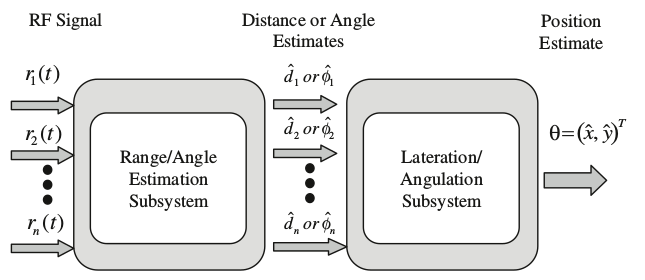
\includegraphics[width=1.0\textwidth]{figures/localization_example.png}
\caption{Classical geolocation system. Range or angle information is extracted from received RF signals. Location is then estimated by lateration/angulation techniques \cite{GeoLoc}.}
\label{fig:2step}
\end{figure*}


In the rest of the section we will provide an overview of the most popular ranging localization methods: TOA, TDOA, AOA, and RSS.



\subsection{Time of Arrival }

Time of Arrival (TOA) localization is a part of class of range-based localization techniques and is often reffered to as tri-lateration. It uses the fact that knowing the propagation speed of  signals between a mobile device and reference points and by measuring the time that a signal takes to be received, the distance can easily be calculated. To obtain an $n$  dimentional position estimate at least $n+1$ range measurements are required. Note that absolute times are used in calculations, so it is critical that the  clocks in base stations and the mobile device are synchronized. It is also assumed that they are all in LOS condition. %Unfortunately, this is not always the case in practice. %In many situation this is not practicle.

Solution techniques developed for range-based localization can be grouped under Maximum Likelihood (ML) and Least Squares (LS) approaches. 
Given the observed range measurements $\Br_n = \Br + \Bw$, the ML estimate $\hat{\Bx}$ of the unknown source location $\Bx$ is obtained by maximizing the conditional probability density function 
\begin{equation}
\nonumber
\hat{\Bx} = \mbox{arg}\max_{\Bx} P\left(\Br_n|\Bx\right)
\end{equation}
where $\Bw$ represents measurement noise. One of the major problems with ML approach is that it requires the knowledge of exact error-free measurements. Another difficulty is that solving for the unknown position extimate is computationally difficult. Many variants and approximations of the original ML has been  developed \cite{Guvenc}, \cite{Guvenc2}, \cite{HoML}.

In LS approaches the source location extimate $\hat{\Bx}$ is found by minimizing the sum of risiduals \cite{GeoLoc}
\begin{equation}
\nonumber
\hat{\Bx} = \mbox{arg}\min_{\Bx} \left\lbrace \sum_{i=1}^m \beta_i\left(r_n^{(i)} - \|\Bx - \Ba_i\|\right)^2 \right\rbrace
\end{equation}
where $a_i$ is a vector of known coordinates of reference points (sensors),   $r_n^{(i)}$ is a range measurement associated with it, $\beta_i$ is a weight
that can be used to emphasize  the degree of confidence in the measurement, and $m$ is a number of sensors.


\subsection{Time Difference of Arrival }

\subsection{Angle of Arrival }

\subsection{Non-Range-Based}

The previously discussed localization methods are all based on determining the distance of a receiver from RF-emitting base stations. This is not the only way localization can be done. For example, inertial tracking systems calculate position without external references. They do this using two types of sensors: accelerometers (which measure instantaneous changes in speed) and gyroscopes (which can be used to measure orientation). Using these sensors and the previous position and orientation, an updated position and orientation can be calculated. ``Dead reckoning'' is the term used to describe such a system which calculates position and orientation using differential measurements of speed and direction.

Inertial systems provide high accuracy over short periods of time, but even with very accurate sensors they are continuously accumulating error which will lead to significant drifts over larger periods of time. RF based methods on the other hand do not accumulate drift, but are susceptible to obstruction by buildings and construction materials. Therefore RF and inertial based localization methods are complementary, because the intertial method continues calculations while the RF signal is lost, and the RF method corrects for drifts over time. In the future hybrid systems are likely to become more popular as they have the potential to be more accurate and robust.

%\subsection{Old}
%
%Review of ranging and localization methods, theory behind it, application, limitations. 
%
%TOA,
% 
%TDOA,
%
%AOA ?,
%
%non-range-based? 
%
%"Geolocation techniques"
%
%\cite{GeoLoc}
%\cite{LiuSurvey}

\section{Contributions and Organization of the Thesis}

\subsection{Contributions  of the Thesis} \label{contributions}


single source localization

something like:

the material developed here / mathematical tools and methods are suitable for many different scenarios 
OR
can have different world life applications, for example: TOA, TDOA, static positioning using UWB range measurements. 

This work mostly investigated possible localization solution for the wireless sensor networks that use radio frequency measurements to obtain the range or range-difference measurements. However, some of the methods presented in this work can also be applied for other mediums, i.e. ultrasonic, sonic, light. 

In this paper, which considers both problems, the main focus is on efficient computation of least squares (LS) estimates of the source’s coordinate vector. The models that we consider for the said vector are based on  the assumption that the sensor network can be used, along with some form of preprocessing, to obtain (noisy) range or range-difference measurements. From a practical standpoint, this is a simplifying assumption (e.g., in nonline-of-sight scenarios), albeit one commonly made in \cite{Cheung} and \cite{classMDS} ([7] and [8]). Even so, the resulting location estimation problems are nonconvex and, therefore, rather difficult to solve globally, which explains why only approximate solutions to them have appeared in \cite{SmithAbel}, ~, \cite{LiHu} ([1], [2], [5],) and \cite{Cheung}. We should also mention here the family of data fusion methods \cite{Sayed} in which linear least squares problems are constructed via subtraction of equations. However, these methods do not provide optimal solutions since they implicitly assume the existence of an error-free measurement. In this paper, we first consider the problem of source localization from range measurements. 


In Section II we provide a result that explains why a recently proposed semidefinite relaxation (SDR) \cite{Cheung} of the R-LS approach to this problem may yield an accurate approximation; however, we also show that the SDR may lead to a poor approximation. For lack of a good solution to the R-LS problem, we then turn our attention to an SR-LS approach. Although the latter approach also leads to a nonconvex problem, we show that this problem can be efficiently and globally solved. Then we go on to consider the source localization problem from range-difference measurements in Section III. Our main results here concern an SRD-LS approach to this problem. In particular, we show that despite the fact that the said SRD-LS problem is also nonconvex, it can be efficiently solved, and we provide the details of an algorithm that computes the global solution of this problem. We end Section III by remarking that an SDR approach applied to a corresponding RD-LS criterion leads to extremely poor solutions. Several numerical examples suggest that the exact SR-LS and SRD-LS solutions can be more accurate by several orders of magnitude than existing approximate SR-LS and SRD-LS estimates, and than SDR-based approximations of the R-LS and
RD-LS solutions.

\subsection{Organization of the Thesis} \label{organization}

\begin{description}
\item[\textbf{Chapter 1}] contains a statement of
the claims which will be proved by this dissertation followed by an overview of the structure of the document itself. Describes in details the open problem which is to be tackled together with its context, its impact and the overall motivation for the research overall.
\item[\textbf{Chapter 2}] IRW-SR-LS.
\item[\textbf{Chapter 3}] PCCP.
\item[\textbf{Chapter 4}] Sequential Relaxation.
\item[\textbf{Chapter 6}] contains a restatement of the claims and results of the dissertation. It also enumerates avenues of future work for further development of the concept and its applications.
\end{description}
%	\startchapter{The Problem to be Solved}
\label{chapter:problem}

TODO

Review of ranging and localization methods, theory behind it, application, limitations: 

TOA,
 
TDOA,

AOA ?,

non-range-based? 
%
%"Geolocation techniques"
%
%UVic thesis template tips:
%
%
%why the problem is important, what its impact is and what its application, if any. Here you are free to elaborate and write as much as you think is necessary to avoid the examination doubt that you have a brilliant new solution to a trivial and unimportant issue.
%
%"The Craft of Research" by Wayne Booth \cite{booth1}, which can be found in the main library at Q180.55 M4B66. From there I have transferred to my writing a fairly simple structure for talking about the topic of the research, with the question to be asked and its motivation and significance. It goes as follows:
%\begin{enumerate}
%\item {\textit{I am trying to learn about (working on, studying...)}}
%\item {\textit{because I want to find out....}}
%\item {\textit{in order to understand...}}
%\end{enumerate}
%
%Another way of looking at this is to ask the
%\textit{what}, \textit{why} and \textit{where}, starting from a \textit{setting} of the problem with a first point A, stating what the \textit{goal} is at point B and having an \textit{action link} between the two which will encompass your new solution. As surprising as this may be to some of you, I found reading a book from Microsoft very useful: "Beyond Bullet Points: Using Microsoft Office PowerPoint 2007 to Create Presentations That Inform" \cite {atkin}. The goal of the book is to improve presentations with Power Point, but there is a lot that can be transferred towards \textit{effective communication} for a thesis.
%
%In summary, my view of the second chapter on
%\textit{"The Problem to be solved"} is as follows:
%\begin{enumerate}
%\item {\textit{Not} all the background and definitions (boring!) - use instead just-in-time explanations as needed in every context as it comes up;}
%\item {Motivation in depth;}
%\item {Tutorial high level explanation, where it is important to choose the right pitch: who is the audience? who are you teaching here?}
%\item {Make it exciting, make it current, make it important - why do I want to keep reading?}
%\item {Should you list here the solutions from other researchers? I think not, list instead the different facets of the problems that other researchers have attacked.}
%\item {A taxonomy can be extremely useful to place your problem and its particular special features within the perfect context of the overall area, as you need to make sure that the reader understands perfectly what you are trying to solve.}
%\end{enumerate}
	%\startchapter{Improved Least-Squares Methods for Source Localization: An Iterative Re-Weighting Approach}
\startchapter{Iterative Re-Weighting Least-Squares Methods for Source Localization}
\label{chapter:irw}

Locating a radiating source from range or range-difference measurements in a passive sensor network has recently attracted an increasing amount of research interest as it finds applications in a wide range of network-based wireless systems. Among the useful localization methods that have been documented over the years, least squares based algorithms constitute an important class of solution techniques as they are geometrically meaningful and often provide low complexity solution procedures with competitive estimation accuracy \cite{SmithAbel} - \cite{BeckStLi}. On the other hand, the error measure in a least squares (LS) formulation for the localization problem of interest is shown to be highly nonconvex, possessing multiple local solutions with degraded performance.  There are many methods for continuous unconstrained optimization \cite{AntonLu}, however most of them are \textit{local} methods that are iterative, hence extremely sensitive to where the iteration begins, and give no guarantee to yield global solutions when applied to non-convex objective functions. In the case of source localization, this inherent feature of local methods is particular problematic because the source location is assumed to be entirely unknown and can appear practically anywhere, thus the chances to secure a good initial point for a local algorithm are next to none. For these reasons, various ``global'' localization techniques were investigated that are either non-iterative or insensitive to initial iterate. One representative in the class of global localization methods is the convex-relaxation based algorithm for range measurements proposed in \cite{Cheung}, where the least squares model is relaxed to a semidefinite programming problem which is known to be convex \cite{VBoyd}, hence robust to where it starts. Another representative in this class is reference \cite{BeckStLi}, where localization problems for  range as well as range difference measurements are addressed by developing solution methods for \textit{squared} range LS (SR-LS) and \textit{squared} range difference LS (SRD-LS) problems. The methods proposed in \cite{BeckStLi} are non-iterative and the solutions obtained are proven to be the global minimizers of the respective SR-LS and SRD-LS problems, which are shown to be excellent estimates of the original LS solutions.

This chapter presents improved least squares methods that demonstrate improved localization performance when compared with the some best known results from the literature. The key new ingredient of the proposed algorithms is an iterative procedure where the SR-LS (SRD-LS) algorithm is iteratively applied to a weighted sum of squared terms where the weights are carefully designed so that the iterates produced quickly converge to a solution which, on comparing with the best known results, is found to be considerably closer to the original range-based (range-difference-based) LS solution. % that is known to be the maximum-likelihood estimator in the case of Gaussian white measurement noise. Numerical results are presented for performance evaluation and comparisons.



\section{Source Localization From Range Measurements}%II
\subsection{Problem Statement}%2.1


The source localization problem considered here involves a given array of $m$ sensors specified by $\{\Ba_1,\ldots, \Ba_m\}$ where $\Ba_i\in R^n$  contains the $n$ coordinates of the $i$th sensor in space $R^n$. Each sensor measures its distance to a radiating source $\Bx\in R^n$. Throughout it is assumed that only noisy copies of the distance data are available, hence the \textit{range measurements} obey the model
\begin{equation} \label{eq:3.1}
\setcounter{equation}{1}
r_i = \|{\Bx} - {\Ba}_i\| + \varepsilon_i, i = 1,\ldots , m.
\end{equation}                                                                                                     	where $\varepsilon_i$ denotes the unknown noise that has occurred when the $i$th sensor measures its distance to source $\Bx$. Let $\Br=[r_1 \ r_2 \ldots r_m]^T$ and $\Beps=[\varepsilon_1 \ \varepsilon_2 \ldots \varepsilon_m]^T$. The source localization problem can be stated as to estimate the exact source location $\Bx$ from the noisy range measurements $\Br$. In the rest of this section, a least-squares (LS) formulation of the localization problem and two most relevant state-of-the-art solution methods are briefly reviewed; and a new method based on iterative re-weighting of squared range LS technique as well as a variant of the proposed method are then presented. %; and numerical results for performance evaluation and comparisons of the relevant algorithms are reported.

%
%The source localization problem considered here involves a given array of $m$ sensors specified by $\{\Ba_1,\ldots, \Ba_m\}$ where $\Ba_i\in R^n$  contains the $n$ coordinates of the $i$th sensor in space $R^n$. Each sensor measures its distance to a radiating source $\Bx\in R^n$. Throughout it is assumed that only noisy copies of the distance data are available, hence the \textit{range measurements} obey the model
%\begin{equation} \label{eq:3.0}
%\setcounter{equation}{1}
%r_i = \|{\Bx} - {\Ba}_i\| + \varepsilon_i, i = 1,\ldots , m.
%\end{equation}                                                                                                     	where $\varepsilon_i$ denotes the unknown noise that has occurred when the $i$th sensor measures its distance to source $\Bx$. Let $\Br=[r_1 \ r_2 \ldots r_m]^T$ and $\Beps=[\varepsilon_1 \ \varepsilon_2 \ldots \varepsilon_m]^T$. The source localization problem can be stated as to estimate the exact source location $\Bx$ from the noisy range measurements $\Br$. 
%
%For the localization problem at hand, the range-based least squares (R-LS) estimate refers to the solution of the problem
%\begin{equation}\label{eq:3.1} %eq 2
%\Min_{\Bx} \quad F(\Bx)=\sum_{i=1}^{m} (r_i - \|{\Bx} - {\Ba}_i\|)^2
%\end{equation}
%
%Formulation (\ref{eq:3.2}) is connected to the maximum-likelihood (ML) location estimation that determines $\Bx$ by examining the probabilistic model of the error vector $\Beps$. If $\Beps$ obeys a Gaussian distribution with zero mean and covariance $\symb{\Sigma} = \mbox{diag}(\sigma_1^2, \ldots, \sigma_m^2)$, then the maximum likelihood (ML) location estimator in this case is known to be
%\begin{equation} \label{eq:3.3}%eq 3
%\Bx_{ML} = \mbox{arg}\!\min_{{\Bx} \in R^n} (\Br - \Bg)^T\Sigma^{-1}(\Br - \Bg)
%\end{equation}
%where $\Bg = [g_1 \ g_2 \ldots \ g_m]^T$ with $g_i = \|{\Bx} - {\Ba}_i\|$. It follows immediately that the ML solution in (\ref{eq:3.3}) is identical to the R-LS solution of problem (\ref{eq:3.2}) when covariance $\symb{\Sigma}$ is proportional to the identity matrix, i.e., $\sigma_1^2=\ldots =\sigma_m^2 = 1$. In the literature this is known as the equal noise power case. For notation the method described in this chapter focuses on the equal noise power case, however the method developed below is also applicable to the unequal noise power case by working on a weighted version of the objective in  (\ref{eq:3.2})  with $\{\sigma_i^{-2}, i = 1, \ldots, m\}$ as the weights.
%
%
%In the rest of this section, a least-squares (LS) formulation of the localization problem and two most relevant state-of-the-art solution methods are briefly reviewed; and a new method based on iterative re-weighting of squared range LS technique as well as a variant of the proposed method are then presented.

\subsection{LS Formulations and Review of Related Work} %2.2

Least squares approaches have proven effective for source localization problems \cite{SmithAbel} -\cite{BeckStLi}. For the localization problem at hand, the range-based least squares (R-LS) estimate refers to the solution of the problem
\begin{equation}\label{eq:3.2} %eq 2
%(R-LS): \Min_{\Bx} \sum_{i=1}^{m} (r_i - \|{\Bx} - {\Ba}_i\|)^2
\Min_{\Bx} f(\Bx) \equiv \sum_{i=1}^{m} (r_i - \|{\Bx} - {\Ba}_i\|)^2
\end{equation}

%\{As could be seen the problem (\ref{eq:3.2}) at hand is nonconvex [].\}
The primary reason that justifies formulation (\ref{eq:3.2}) is its connection to the maximum-likelihood location estimation that determines $\Bx$ by examining the probabilistic model of the error vector $\Beps$. Assuming the errors $\varepsilon_i$ are independent identically distributed (Gaussian) variables with zero mean and variance $\sigma_i^2$, then $\Beps$ obeys a Gaussian distribution with zero mean and covariance $\symb{\Sigma} = \mbox{diag}(\sigma_1^2, \ldots, \sigma_m^2)$, and the maximum likelihood (ML) location estimator in this case is known to be
\begin{equation} \label{eq:3.3}%eq 3
\Bx_{ML} = \mbox{arg}\!\min_{{\Bx} \in R^n} (\Br - \Bg)^T\Sigma^{-1}(\Br - \Bg)
\end{equation}
where $\Bg = [g_1 \ g_2 \ldots \ g_m]^T$ with
\begin{equation} \label{eq:3.4}%eq 4
g_i = \|{\Bx} - {\Ba}_i\|
\end{equation}
It follows immediately that the ML solution in (\ref{eq:3.3}) is identical to the R-LS solution of problem (\ref{eq:3.2}) when covariance $\symb{\Sigma}$ is proportional to the identity matrix, i.e., $\sigma_1^2=\ldots =\sigma_m^2$. In the literature this is known as the equal noise power case. For notation simplicity the method described in this chapter focuses on the equal noise power case, however the method developed below is also applicable to the unequal noise power case by working on a weighted version of the objective in  (\ref{eq:3.2})  with $\{\sigma_i^{-2}, i = 1, \ldots, m\}$ as the weights.

Although there are many methods for continuous unconstrained optimization \cite{AntonLu}, most of them are \textit{local} methods in the sense they are sensitive to the choice of initial point where the iteration of an optimization algorithm begins. Especially when applied to a nonconvex objective function which possesses a number of local minimizers, unless a chosen local method starts at an initial point that happens to be sufficiently close to the (unknown) global minimizer, the solution obtained by the method gives no guaranty about its global minimality. Unfortunately, the objective in (\ref{eq:3.2}) is highly nonconvex, possessing many local minimizers even for small-scale systems. As an example, consider an instance of the source localization problem on the plane $n = 2$ with five sensors $ m = 5$ located at $(6,4)^T, (0,-10)^T, (5,-3)^T, (1,-4)^T$ and  $(3,-3)^T$ with the source emmitting the signal at $\Bx_s = (-2,3)^T$. Figure (\ref{fig:ExampleOfRLSNonconvexity}) describes a contour plot of the R-LS objective function in (\ref{eq:3.2}) over the region $\Re = \{\Bx: -6 \leq x_1 \leq 13, -10 \leq x_2 \leq 9 \}$. It can be observed from the plot that there are two minimizers at $\tilde{\Bx} = (-1.9907, 3.0474)^T$ and $\widehat{\Bx} = (11.1152, -2.6785)^T$ with values of the objective  $f(\tilde{\Bx}) = 0.1048 $ and $f(\widehat{\Bx}) = 15.0083$ respectively. As expected, the global minimizer of R-LS objective offers a good approximation of the exact source location $\Bx_s$, but is unlikely to be precisely at point $\Bx_s$ because the objective $f(\Bx)$ is defined using noisy range measurements. Note that for the exact source location $\Bx_s$ we have $f(\Bx_s) = \sum_{i=1}^m \varepsilon_i^2$.

\begin{figure*}[t]
\centering
  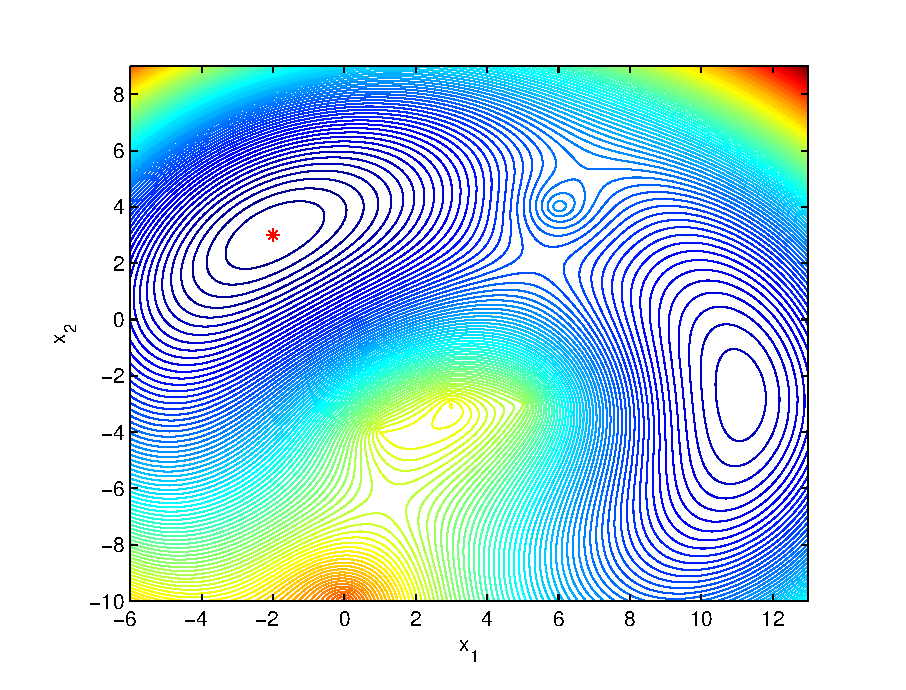
\includegraphics{figures/nonconvexity_example_ls_new_range}
\caption{Contours of the R-LS objective function over the region $\protect\Re = \protect\lbrace \protect\Bx:-6\protect\leq x_1 \protect\leq 13, -10\protect\leq x_2 \protect\leq 9 \protect\rbrace$}
\label{fig:ExampleOfRLSNonconvexity}
\end{figure*}

Reference \cite{Cheung} addresses problem (\ref{eq:3.2}) by a convex relaxation technique where (\ref{eq:3.2}) is modified to a convex problem known as semidefinite programming (SDP) \cite{VBoyd}. A key step in this procedure is to use (\ref{eq:3.4}) with  $g_i$ as new variables, which leads (\ref{eq:3.2}) to the constrained problem
\begin{eqnarray} \label{eq:3.5}%eq 5 a,b
\setcounter{abc}{1}
\Min_{{\Bx}, {\Bg}} \sum_{i=1}^m (r_i - g_i)^2\qquad\\
\stepcounter{abc} \setcounter{equation}{5} 
\mbox{subject to: \ } g_i^2=\|{\Bx} - {\Ba_i}\|^2,\quad i = 1, \ldots,m.
\end{eqnarray}
By further defining matrix variables
\begin{equation} \label{eq:3.6}%eq 6
\setcounter{abc}{0}
\BG = \left[\begin{array}{c} \Bg \\
1 \end{array}\right] \left[ \begin{array}{cc} \Bg^T & 1 \end{array} \right] \mbox{and } \BX = \left[\begin{array}{c} \Bx \\
1 \end{array}\right] \left[ \begin{array}{cc} \Bx^T & 1 \end{array} \right]
\end{equation}
and neglecting the rank constrains on $\BG$ and $\BX$, (\ref{eq:3.5}) can be reformulated in term of variables $\BG$ and $\BX$ as
\begin{eqnarray}
\setcounter{abc}{0}
\label{eq:3.7}
\setcounter{abc}{0} % before was 12, now change to 7 - WSLU
\setcounter{abc}{1}\setcounter{equation}{7}
\Min_{\BX,\BG} \sum_{i=1}^{m} \left(G_{ii}- 2r_iG_{m+1,i}+r_i^2\right)\qquad\\
\stepcounter{abc}\setcounter{equation}{7}
\mbox{subject to: \ } G_{ii}=\boldmath{Tr}\left(\BC_i\BX\right), i = 1, \ldots,m \\
\stepcounter{abc}\setcounter{equation}{7}
\BG \succeq 0, \BX \succeq 0 \quad\qquad\qquad\qquad\\
\stepcounter{abc}\setcounter{equation}{7}
G_{m+1,m+1}=G_{n+1,n+1}=1 \quad
\end{eqnarray}
where
\begin{equation} \label{eq:3.8} % put here as 8
\setcounter{abc}{0}
\setcounter{equation}{8}
C_i=\left( \begin{array}{cc}  \BI\!_{n\times n} & -\Ba_i
\\ -\Ba_i^T & \|\Ba_i\|^2 \\
\end{array}\right) \quad i=1,\ldots,m
\end{equation}
which is a standard SDP problem that can be solved efficiently \cite{VBoyd,AntonLu}. Note that because (\ref{eq:3.7}) is a convex problem, global minimality of the solution is ensured regardless of the initial point used. On the other hand, however, because (\ref{eq:3.7}) is an approximation of the original problem in (\ref{eq:3.2}), the solution of (\ref{eq:3.7}) is only an approximate solution of problem (\ref{eq:3.2}). In what follows the solutions obtained by this SDP-relaxation based method will be referred to as SDR-LS solutions.

A rather different approach is recently proposed in \cite{BeckStLi} where the localization problem (\ref{eq:3.2}) is tackled by developing techniques that find global solution of the \textit{squared range based LS} (SR-LS) problem
\begin{equation} \label{eq:3.9}%eq 9
\Min_{\Bx} \sum_{i=1}^{m} \left(\|{\Bx} - {\Ba}_i\|^2 - r_i^2\right)^2
\end{equation}
By writing the objective in (\ref{eq:3.9}) as $\left(\alpha-2\Ba_i^T\Bx+\|\Ba_i\|^2-r_i^2\right)^2$ with $\alpha=\|\Bx\|^2$, it becomes a convex quadratic objective if one treats $\alpha$  as an additional variable and  $\alpha=\|\Bx\|^2$  as a constraint. In this way, (\ref{eq:3.9}) is converted to the following constrained LS problem after necessary variable changes:
\begin{eqnarray} \label{eq:3.10}
\setcounter{abc}{1}
\Min_{{\By} \in R^{n+1}} \|\BA\By-\Bb\|^2 \qquad\\
\stepcounter{abc} \setcounter{equation}{10} \mbox{subject to: \ }
\By^T\BD\By + 2\Bf^T\By = 0
\end{eqnarray}
where $\By = [\Bx^T \|\Bx\|^2]^T$ and
\setcounter{abc}{0}
\begin{equation} \label{eq:3.11}
\setcounter{abc}{0}
\setcounter{equation}{11}
\BA=\left(\begin{array}{cc}
    -2\Ba_1^T & 1 \\
    \vdots  & \vdots \\
    -2\Ba_m^T & 1
    \end{array} \right),
\Bb=\left(\begin{array}{c}
    r_1^2-\|\Ba_1\|^2 \\
    \vdots \\
    r_m^2-\|\Ba_m\|^2
    \end{array} \right)
\end{equation}
\begin{equation}% \label{eq:3.12}
\nonumber
\BD=\left(\begin{array}{cc}
    \BI\!_{n\times n} & \BO_{n\times n} \\
    \BO_{n\times n} & 0
    \end{array} \right),
\Bf=\left(\begin{array}{c}\BO \\ -0.5 \end{array} \right)
\end{equation}
This problem conversion, made in \cite{BeckStLi}, turns out to be crucial as problem (\ref{eq:3.10}), which remains to be nonconvex because of the nonlinear equality constraint (\ref{eq:3.10}b), falls into the class of generalized trust region subproblems (GTRS) \cite{More, FortinWol}  whose global solutions can be computed by exploring the KKT conditions which are both necessary and sufficient optimality conditions in the case of GTRS \cite{More}.

Few remarks are now in order. First, an unconstrained version of (\ref{eq:3.10}) may be obtained by neglecting the constraint in (\ref{eq:3.10}b) as
\begin{equation} \label{eq:3.12}%eq 13
\Min_{{\By} \in R^{n+1}} \|\BA\By-\Bb\|^2
\end{equation}
whose solution, called \textit{unconstrained squared-range-based LS }(USR-LS) estimate, is given by
\begin{equation} \label{eq:3.13}%eq 14
\By^*=\left(\BA^T\!\BA\right)^{-1}\!\!\!\!\BA^T\Bb
\end{equation}
It is demonstrated by numerical experiments \cite{BeckStLi} that the SR-LS solution outperforms the USR-LS and, in many cases, SDR solutions. Second, the SR-LS solution, although it solves (\ref{eq:3.9}) exactly, lacks the statistical interpretation of the ML formulation. The SR-LS remains to be an approximate solution for the original problem in (\ref{eq:3.2}) and, as it was demonstrated by the numerical results in \cite{BeckTeCh} and \cite{BeckGPS}, provides less accurate estimates of the true source location, than the LS estimate. The method, described in detail below, tries to reduce the gap between the two solutions.

\subsection{An Iterative Re-Weighting Approach}%2.3

%An iterative re-weighting minimization schemes in several forms has been proposed in the literature \cite{BeckTeCh}, \cite{Beck15}. The standard fixed point (SFP) algorithm \cite{BeckTeCh} was constructed similarly to the Weizfeld method that was designed to solve the Fermat-Weber problem. The iterates of SPF were constructed from the optimality conditions for (\ref{eq:3.2}). SPF is a gradient method with a fixed step size. Proposed schemes for choosing the initial point $\Bx_0$ guarantees the convergence and eliminates points of non-smoothness
%and the sequential weighted least squares algorithms (SWLS) \cite{BeckTeCh} are based 

Iterative re-weighting least squares method is a popular technique used for solving problems involving the sums of norms $\{cite\}$. The method has found many applications, such as in robust regression $\{cite\}$, sparse recovery $\{cite\}$, but the most relevand application for the current case is for solving the Fermat-Weber location problem. The Fermat--Weber problem %is one of the oldest easily-stated nontrivial problems in computational geometry: 
has a long history and has been extensively studied in the field of optimization and location theory $\{cite\}$. This problem can be stated as: given $m$ points $\Ba_1, \Ba_2, \ldots, \Ba_m \in R^n$ called \textit{ancors} and nonnegative weights $\omega_1, \omega_2, \ldots, \omega_m > 0$, find $\Bx \in R^n$ that minimizes the weighted sum of Euclidian distances between $\Bx$ and $m$ ancors:
\begin{equation} \label{eq:FW}
\nonumber
\Min_{\Bx \in R^n} \sum_{i=1}^{m} \omega_i\|\Bx - \Ba_i\|.
\end{equation}
Fermat--Weber problem is much easier to analyze and solve than the ML problem (\ref{eq:3.2}) since it is a well-structured
nonsmooth convex minimization problem, however the similarities of these problems has been noted in the literature \cite{BeckTeCh}.
%This problem has a long history and has been extensively studied in the field of optimization and location theory.
%the most famous and oldest example of the IRLS method is Weiszfeld’s method for solving the Fermat–Weber problem — an algorithm that was introduced in 1937.
% Our objective here is to mimic the Weiszfeld algorithm [16] to obtain an algorithm for solving the nonsmooth and nonconvex ML problem (1.2). The Weiszfeld method is a very simple fixed-point scheme that is designed to solve the Fermat–Weber problem. One way to derive it is to write the first order global optimality conditions for the convex problem (2.1)
The standard fixed point (SFP) algorithm proposed in \cite{BeckTeCh} is a gradient method with a fixed step size. However, being a gradient method, it has chances to converge to local minimum. The sequential weighted least squares algorithm (SWLS) proposed in \cite{BeckTeCh} is also an iterative method where each iteration involves solving a nonlinear least squares problem similar to (\ref{eq:3.9}). As discussed in  \cite{BeckTeCh} the SWLS method is superior over SFP in terms of convergence rate and a wider region of convergence to the global minimum. However, it still does have a chance to converge to a local minimum in case of certain sensor setup even if an initial point $\Bx_0$ is constructed by following a procedure developed specifically for this purpose. The method presented below is different from the above described approaches in a sense that it does not require an initial point and the solution produced is guranteed to converge to a \textit{global} solution. 

\subsubsection{Weighted squared range-based least squares formulation} %2.3.1

We now consider a weighted SR-LS (WSR-LS) problem, namely,
\begin{equation} \label{eq:3.14} %eq 15
\Min_{\Bx} \sum_{i=1}^{m} w_i\left(\|{\Bx} - {\Ba}_i\|^2 - r_i^2\right)^2
\end{equation}
Following \cite{BeckStLi}, it is rather straightforward to convert (\ref{eq:3.14}) into a GTRS similar to (\ref{eq:3.10}) as
\begin{eqnarray} \label{eq:3.15} %eq 16 a,b
\setcounter{abc}{1}
\Min_{{\By} \in R^{n+1}} \|\BGA\left(\BA\By-\Bb\right)\|^2 \qquad\\
\stepcounter{abc} \setcounter{equation}{15} \mbox{subject to: \ }
\By^T\BD\By + 2\Bf^T\By = 0
\end{eqnarray}
where $\BGA=\mbox{diag}\left(\sqrt{w_1},\ldots,\sqrt{w_m}\right)$. Clearly, problem (\ref{eq:3.15}) can be written as
\begin{eqnarray}
\setcounter{abc}{0}
\label{eq:3.16}%eq 17 a,b
\setcounter{abc}{1}
\Min_{{\By} \in R^{n+1}} \|\BA_w\By-\Bb_w\|^2 \qquad\\
\stepcounter{abc} \setcounter{equation}{16} \mbox{subject to: \ }
\By^T\BD\By + 2\Bf^T\By = 0
\end{eqnarray}
where $\BA_w = \BGA\BA$ and $\Bb_w=\BGA\Bb$. On comparing (\ref{eq:3.16}) with (\ref{eq:3.10}), %we conclude that 
if $S(\BA,\Bb,\BD,\Bf)$ denotes a solver that produces the global solution of problem (\ref{eq:3.10}) for a given data set $\{\BA,\Bb,\BD,\Bf\}$, then the same solver produces the global solution of the weighted problem (\ref{eq:3.14}) as long as it is applied to the data set $\{\BA_w,\Bb_w,\BD,\Bf\}$. We stress that the weights $\{w_i, i=1,\ldots, m\}$ in (\ref{eq:3.14}) are \textit{fixed} nonnegative constants.


\subsubsection{Moving the SR-LS solution towards R-LS solution via iterative re-weighting}% 2.3.2

The main idea here is to use the weights $\{w_i, i=1,\ldots, m\}$  to tune the objective in (\ref{eq:3.14}) toward the objective in (\ref{eq:3.2}) so that the solution obtained by minimizing such a WSR-LS objective is expected to be closer toward that of the problem (\ref{eq:3.2}). To substantiate the idea, we compare the $i$th term of the objective in (\ref{eq:3.14}) with its counterpart in (\ref{eq:3.2}), namely,
\begin{equation} \label{eq:3.17} %eq 18
\setcounter{abc}{0}
\underbrace{w_i\left(\|\Bx-\Ba_i\|^2-r_i^2\right)^2}_{\mbox{in (15)}}\leftrightarrow\underbrace{\left(\|\Bx-\Ba_i\|-r_i\right)^2}_{\mbox{in (2)}}
\end{equation}
and write the term in (\ref{eq:3.14}) as
\begin{equation} %\label{eq:3.18}%eq19
\nonumber
\begin{array}{l}
w_i\left(\|\Bx-\Ba_i\|^2-r_i^2\right)^2 = \\ w_i\left(\|\Bx-\Ba_i\|+r_i\right)^2 \underbrace{\left(\|\Bx-\Ba_i\|-r_i\right)^2}_{\mbox{same as in (2)}}
\end{array}
\end{equation}
It follows that the objective in (\ref{eq:3.14}) would be the same as in (\ref{eq:3.2}) if the weights $w_i$ were assigned to $1/\left(\|\Bx-\Ba_i\|+r_i\right)^2$. Evidently, weight assignments as such cannot be realized because $w_i$'s must be fixed constants for (\ref{eq:3.14}) to be a globally solvable WSR-LS problem. A natural remedy to deal with this technical difficulty is to employ an iterative procedure whose $k$th iteration generates a global solution $\Bx_k$  of a WSR-LS sub-problem of the form
\begin{equation}\label{eq:3.19}% eq20
\Min_{x} \sum_{i=1}^m w_i^{(k)}\left(\|\Bx-\Ba_i\|^2-r_i^2\right)^2
\end{equation}
where for $k\geq2$ the weights $\{w_i^{(k)},i=1,\ldots,m\}$ are assigned using the previous iterate $\Bx_{k-1}$ as
\begin{equation} \label{eq:3.20}%eq 21
w_i^{(k)}=\frac{1}{\left(\|\Bx_{k-1}-\Ba_i\|+r_i\right)^2}
\end{equation}
while for $k=1$ all weights $\{w_i^{(1)}, i=1,\ldots, m\}$ are set to unity. Clearly the weights given by (\ref{eq:3.20}) are realizable. More importantly, when the iterates produced by solving (\ref{eq:3.19}) (namely $\Bx_k$ for $k = 1, 2,\ldots$) converge, in the $k$th iteration with $k$ sufficiently large, the objective function of (\ref{eq:3.19}) in a small vicinity of its solution $\Bx_k$ is approximately equal to
\begin{equation} \label{sr:w}
\nonumber
\begin{aligned}
&\sum_{i=1}^m w_i^{(k)}\left(\|\Bx-\Ba_i\|^2-r_i^2\right)^2 \\
 \approx &\sum_{i=1}^m w_i^{(k)}\left(\|\Bx_k-\Ba_i\|^2-r_i^2\right)^2 \\
 =&\sum_{i=1}^m w_i^{(k)}\left(\|\Bx_k-\Ba_i\|+r_i\right)^2\left(\|\Bx_k-\Ba_i\|-r_i\right)^2  \\
 \approx &\sum_{i=1}^m w_i^{(k)}\left(\|\Bx_{k-1}-\Ba_i\|+r_i\right)^2\left(\|\Bx_k-\Ba_i\|-r_i\right)^2 \\
 =&\sum_{i=1}^m \left(\|\Bx_k-\Ba_i\|-r_i\right)^2 \approx \sum_{i=1}^m \left(\|\Bx-\Ba_i\|-r_i\right)^2\\
\end{aligned}
\end{equation}
%In other words, after infinite amount of iterations the WSR-LS solution to the problem (\ref{eq:3.19}) is expected to converge to the global solution of problem (\ref{eq:3.2}). [ Would this wording
In words, with the weights from (\ref{eq:3.20}), the limiting point of the iterates produced by iteratively solving WSR-LS problem (\ref{eq:3.19}) is expected to be close to the global solution of problem (\ref{eq:3.2}).

The algorithmic steps of the proposed localization method are outlined as follows.

\phantom{m}
\framebox{%
\parbox{5.5in}{
\noindent \textbf{Algorithm 1} \label{alg:r-ls}

1) Input data: Sensor locations $\{\Ba_i, i=1,\ldots,m\}$, range measurements $\{r_i, i=1,\ldots,m\}$, maximum number of iterations $k_{max}$ and convergence tolerance $\zeta$.

2) Generate data set $\{\BA,\Bb, \Bd, \Bf \}$ as
\begin{equation} 
\nonumber
\BA=\left(\begin{array}{cc}
    -2\Ba_1^T & 1 \\
    \vdots  & \vdots \\
    -2\Ba_m^T & 1
    \end{array} \right),
\Bb=\left(\begin{array}{c}
    r_1^T-\|\Ba_1\|^T \\
    \vdots \\
    r_m^T-\|\Ba_m\|^T
    \end{array} \right)
\end{equation}
\begin{equation} 
\nonumber
\BD=\left(\begin{array}{cc}
    \BI\!_{n\times n} & \BO_{n\times n} \\
    \BO_{n\times n} & 0
    \end{array} \right),
\Bf=\left(\begin{array}{c}\BO \\ -0.5 \end{array} \right) .
\end{equation}

Set $k=1, w_i^{(1)}=1$ for $i=1,\ldots,m$.

3) Set $\BGA_k=\mbox{diag}\left(\sqrt{w_1^{(k)}},\ldots,\sqrt{w_m^{(k)}}\right)$, $\BA_w=\BGA_k\BA$ and $\Bb_w=\BGA_k\Bb$.

4) Solve the WSR-LS problem 
% 3.20
\begin{equation} 
\nonumber 
\Min_{x} \sum_{i=1}^m w_i^{(k)}\left(\|\Bx-\Ba_i\|^2-r_i^2\right)^2
\end{equation}
via (\ref{eq:3.16})
% 3.21
\begin{equation}
\nonumber
\begin{aligned}
&\Min_{{\By} \in R^{n+1}} \|\BA_w\By-\Bb_w\|^2 \\
&\mbox{subject to: \ }  \By^T\BD\By + 2\Bf^T\By = 0
\end{aligned}
\end{equation} 
to obtain its global solution $\Bx_k$.

5) If $k=k_{max}$ or $\|\Bx_k-\Bx_{k-1}\|<\zeta$, terminate and output $\Bx_k$ as the solution; otherwise, set $k=k+1$, update weights $\{w_i^{(k)}, i=1,\ldots,m\}$ using % 3.21
\begin{equation}
\nonumber
w_i^{(k)}=\frac{1}{\left(\|\Bx_{k-1}-\Ba_i\|+r_i\right)^2}
\end{equation}
and repeat from Step 3).
}
}

\phantom{m}

From the steps in Algorithm 1, it follows that the complexity of the algorithm is practically equal to the complexity of the WSR-LS solver involved in Step 4 times the number of iterations, $k$. The algorithm converges with a small number of iterations, typically a $k\leq6$  suffices. For simplicity, the solutions obtained from Algorithm 1 are called IRWSR-LS solutions. Technical details on how to solve (\ref{eq:3.20}) can be found in Appendix 1.

\subsubsection{A variant of Algorithm 1}% 2.3.3

As argued above, the IRWSR-LS solution from Algorithm 1 is expected to be an improved approximation of the global solution of R-LS problem in (\ref{eq:3.2}). However a small gap between the two solutions is inevitable owing to the approximate nature of the re-weighting strategy. This section presents a variant of Algorithm 1 that closes this gap by taking the IRWSR-LS solution as an initial point to run a good local unconstrained optimization algorithm for problem (\ref{eq:3.2}).  The rationale behind this two-step approach is that the initial point produced in the first step by Algorithm 1 is highly likely within a sufficiently small vicinity of the exact global solution of problem (\ref{eq:3.2}), hence a good local method will lead it to the exact solution in a small number of iterations. We remark that such a ``hybrid'' approach is also expected to work with other ``global'' methods including the SDR-LS and SR-LS methods, but with a difference that employing an IRWSR-LS solution in the first step improves the closeness of the initial point, hence increases the likelihood of securing the exact global solution of problem (\ref{eq:3.2}) by a local method in the second step.

The well-known Newton algorithm \cite{AntonLu} is chosen as a local method because of its fast convergence and low complexity. We note that, unlike in a general scenario where the Newton algorithm is often considered numerically expensive because it requires to compute the inverse of the Hessian matrix, computing such an inverse is not costly in the present case because the dimension of the unknown vector x is extremely low: $n = 2$ or 3. Moreover, the Hessian matrix involved can be efficiently evaluated by a closed-form formula, as shown below.

To evaluate the Hessian of the objective $f(\Bx)$ in (\ref{eq:3.2}), we assume $\Bx\neq\Ba_i$  for $i = 1, \ldots, m$, so that $f(\Bx)$  is a smooth function of $\Bx$. The assumption simply means that the radiating source is away from the sensor at least by a certain distance, which appears to be reasonable for a practical localization problem. Under this circumstance, the gradient and Hessian of $f(\Bx)$ are found to be
\begin{equation}\label{eq:grls}
\setcounter{abc}{1}
\Bg(\Bx)=\sum_{i=1}^m\left(1-\frac{r_i}{\|\Bx-\Ba_i\|})\right)\left(\Bx-\Ba_i\right)
\end{equation}
and
\begin{equation}
\setcounter{equation}{20}
\stepcounter{abc}
\BH(\Bx)=2\left(\tau\BI+\BH_1(\Bx)\right)
\end{equation}
respectively, where
\begin{equation}
\nonumber
\tau=m-\sum_{i=1}^m \frac{r_i}{\|\Bx-\Ba_i\|}
\end{equation}
and
\begin{equation}
\nonumber
\setcounter{abc}{0}
\BH_1(\Bx)=\sum_{i=1}^m \frac{r_i(\Bx-\Ba_i)(\Bx-\Ba_i)^T}{\|\Bx-\Ba_i\|^3}.
\end{equation}
To ensure a descent Newton step, the positive definiteness of the Hessian $\BH(\Bx)$ needs to be examined and, in case $\BH(\Bx)$ is not positive definite, to be modified to guatrantee its positive definiteness. To this end, the eigen-decomposition of $\BH(\Bx)$, namely,
\begin{equation}
\nonumber
\BH(\Bx)=\BU\BLA\BU^T
\end{equation}
may be performed, where $\BU$ is orthogonal and $\BLA=\mbox{diag}\left(\tau+\right.$ $\left.\lambda_1,\ldots, \tau+\lambda_n\right)$  with $\{\lambda_i,i=1,\ldots,n\}$ being eigenvalues of $\BH_1(\Bx)$. Let $l_{min}$  be the smallest eigenvalue of $\BH(\Bx)$, namely $l_{min}=\mbox{min}\left(\tau+\lambda_1,\ldots, \tau+\lambda_n\right)$.  If  $l_{min}>0$, then $\BH(\Bx)$  is positive definite and the Newton algorithm is carried out without modification; if $l_{min}\leq0$, then the algorithm uses a slightly modified Hessian given by
\begin{equation}
\nonumber
\tilde{\BH}(\Bx)=\BU\tilde{\BLA}\BU^T
\end{equation}
where $\tilde{\BLA}=\mbox{diag}\left(\tilde{\lambda}_1,\ldots, \tilde{\lambda}_n\right)$
\begin{equation}
\nonumber
\tilde{\lambda}_i=\left\{\begin{array} {lll}
    \tau+\lambda_i & \mbox{if } \tau+\lambda_i>0 & \\
    \delta &  \mbox{if } \tau+\lambda_i\leq0 & i=1,\ldots,m \end{array} \right.
\end{equation}
and $\delta$ a small positive constant. Obviously, $\tilde{\BH}(\Bx)$ is guaranteed to be positive definite. The search direction in the $k$th iteration of the modified Newton algorithm is given by 
\begin{equation}
\nonumber
\Bd_k = - \BU\tilde{\BLA}^{-1}\BU^T g(\Bx_k)
\end{equation}
where $g(\Bx_k)$ is given by (\ref{eq:grls}). In what follows, solutions obtained by the proposed two-step method are called \textit{hybrid} IRWSR-LS solutions.

\subsection{Numerical Results}

\begin{table}
\centering
\caption{MSE of position estimation for SR-LS, IRWSR-LS and \textit{hybrid} IRWSR-LS methods}
\begin{tabular}{|c|c|c|c|} \hline
\centering
$\sigma$ & SR - LS & IRWSR-LS (Im.,\%) & \textit{hybrid} IRWSR-LS (Im.,\%) \\ \hline
%&&& \\ 
1e-03&	2.0325e-06&	1.1996e-06 (41)	& 1.1994e-06 (41)\\ &&&\\
1e-02&	1.8372e-04&	1.2480e-04 (32)	& 1.2481e-04 (32)\\ &&&\\
1e-01&	1.8361e-02&	1.2223e-02 (33)	& 1.2214e-02 (33)\\ &&&\\
1e+0&	2.3752e+00&	1.5108e+00 (36)	& 1.5330e+00 (35)\\ %&&&&\\
\hline
\end{tabular}
\label{tab:1}
\end{table}

Performance of the proposed algorithms was evaluated and compared with existing state-of-the-art methods by Monte Carlo simulations with a set-up similar to that of \cite{BeckStLi}. SR-LS and SRD-LS solutions were used as performance benchmarks for Algorithm 1 and its variant. In both cases the system consisted of $m$ sensors $\{\Ba_i, i=1, 2,\ldots,m\}$ randomly placed in the planar region in $R^2$, and a radiating source $\Bx_s$, located randomly in the region \textit{R}=$\{\Bx:(x_1,x_2)^T, -10\leq x_1,x_2\leq 10\}$. Coordinates of the source and sensors were generated for each dimension following a uniform distribution. Measurement noise $\{\varepsilon_i, i=1,\ldots,m\}$ was modelled as independent and identically distributed (i.i.d) random variables with zero mean and variance $\sigma^2$. Accuracy of source location estimation was evaluated as the average of the squared position error $\|\Bx^* - \Bx_s\|^2$ where $\Bx_s$ denotes the exact source location and $\Bx^*$ is its estimation obtained by SR-LS, IRWSR-LS and hybrid-IRWSR-LS methods, respectively. Table \ref{tab:1} provides comparisons of these methods with SR-LS. Each table entry is a MSE averaged over 1,000 Monte Carlo runs of a given method for a given noise level. For the columns representing performance of the IRWSR-LS and \textit{hybrid} IRWSR-LS methods each table entry lists their MSE and relative improvement over SR-LS solutions in percentage, in the format: MSE($\%$ Improvement). 

%Second and third column represent a MSE of the IRWSR-LS and \textit{hybrid} IRWSR-LS methods and their relative improvement over SR-LS solutions in percentage, in the format: relative error($\%$ Improvement). 
%The last column in each table represents relative improvement of the proposed methods over SR-LS(SRD-LS) solutions in percentage.

Employing a set-up similar to that in \cite{BeckStLi}, the simulation studies of Algorithm 1 and its variant considered $m = 5$ sensors placed in the region $[-15;15]\times[-15;15]$, with $\sigma$ being one of four possible levels $\{10^{-3}, 10^{-2}, 10^{-1}, 1\}$. The range measurements $\{r_i, i=1, 2,\ldots,5\}$ were calculated using (\ref{eq:3.1}) and Step 4 of Algorithm 1 was implemented using the SR-LS algorithm proposed in \cite{BeckStLi}. It is observed that IRWSR-LS solutions offer considerable improvement over SR-LS solutions, and, as expected, in most cases hybrid IRWSR-LS solutions provide further but only incremental improvement. This is not surprising because the IRWSR-LS solutions themselves are already fairly close to the solutions of problem (\ref{eq:3.2}). It should also be noted again that for the exact source location $\Bx_s$ we have $f(\Bx_s) = \sum_{i=1}^m \varepsilon_i^2$. One might argue that the SR-LS solution already provides a rather good approximation for R-LS in the sense that SR-LS and IRWSR-LS (hybrid IRWSR-LS) have the same order of magnitude of the mean squared error. However, further analysis of the data that was used to generate Table \ref{tab:1} illustrates the advantage of the IRWSR-LS (hybrid IRWSR-LS) solution over the SR-LS.

Each entry in Table \ref{tab:2} is a standard deviation of the squared  estimation errors  aggregated over the  same 1,000 Monte Carlo runs described above in Table \ref{tab:1} (where the MSE of the position estimation are shown). The results summarised in Table \ref{tab:2} suggest that, again, IRWSR-LS and hybrid IRWSR-LS outperform SR-LS. Figures (\ref{fig:Noise03IRW} - \ref{fig:Noise00IRW}) describe the histograms of the location estimation errors $\|\Bx^* - \Bx_s\|$ of the SR-LS solution (left images) and IRWSR-LS (right images) for all four noise levels with $\sigma$ being one of $\{10^{-3}, 10^{-2}, 10^{-1}, 1\}$. Here $\Bx^*$ denotes the estimated location and $\Bx_s$ is the exact location of the source. Histograms that correspond to the results obtained by IRWSR-LS are shifted closer towards $0$ than those obtained by SR-LS and have smaller variance. Also, the solutions obtained by running IRWSR-LS have fewer outliers with large error.



\begin{table}
\centering
\caption{Standard deviation of the squared estimation error for SR-LS, IRWSR-LS and \textit{hybrid} IRWSR-LS methods}
\begin{tabular}{|c|c|c|c|} \hline
$\sigma$ & SR - LS & IRWSR-LS & \textit{hybrid} IRWSR-LS \\ \hline
%&&& \\ 
1e-03&	6.3438e-06&	2.0843e-06 & 2.0864e-06\\ &&&\\
1e-02&	3.2575e-04&	2.0530e-04 & 2.0530e-04\\ &&&\\
1e-01&	4.6998e-02&	2.1377e-02 & 2.1377e-02\\ &&&\\
1e+0&	1.1920e+00&	4.3266e+00 & 4.3266e+00\\ %&&&&\\
\hline
\end{tabular}
\label{tab:2}
\end{table}



\begin{figure}%[t]
\centering
  \makebox[\textwidth][c]{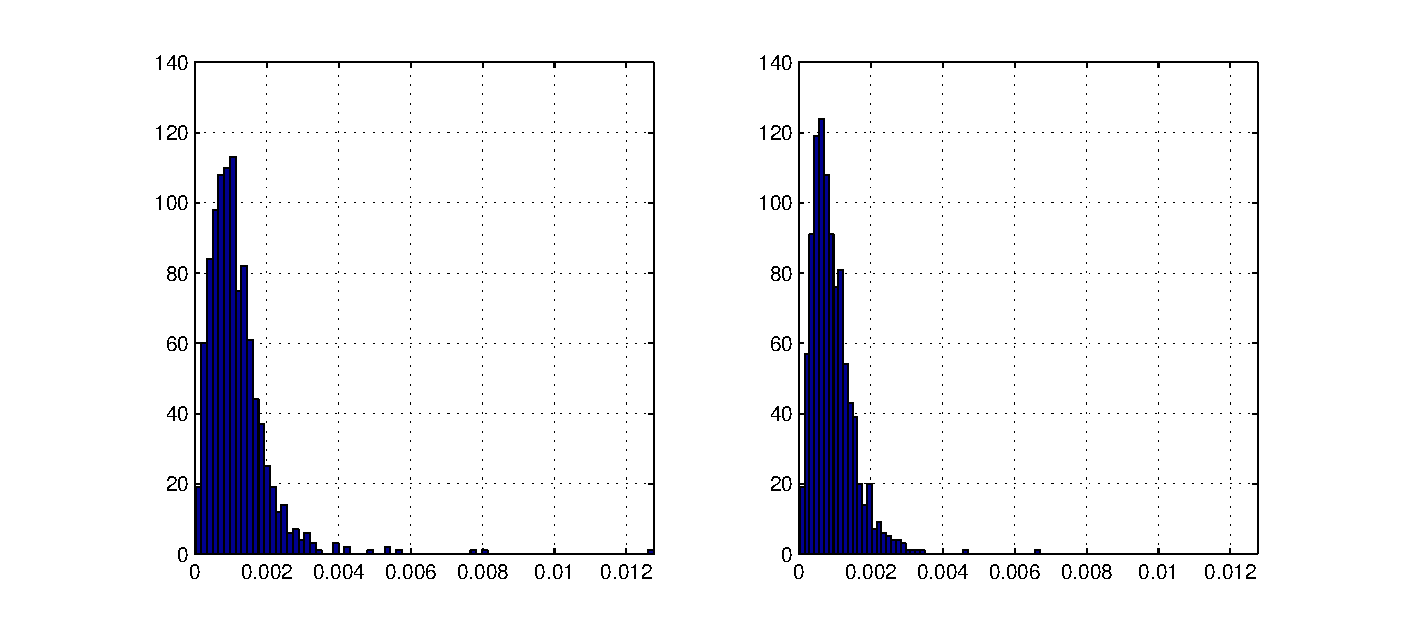
\includegraphics[width=1.2\textwidth]{figures/range_IRWLS/Noise03LeftBeckRightIrw}}
\caption{Histograms of the errors of the SR-LS (left) and IRWSR-LS (right) solutions, noise $\protect\sigma = 10^{-3}$}
\label{fig:Noise03IRW}
\end{figure}

\begin{figure}%[t]
\centering
  \makebox[\textwidth][c]{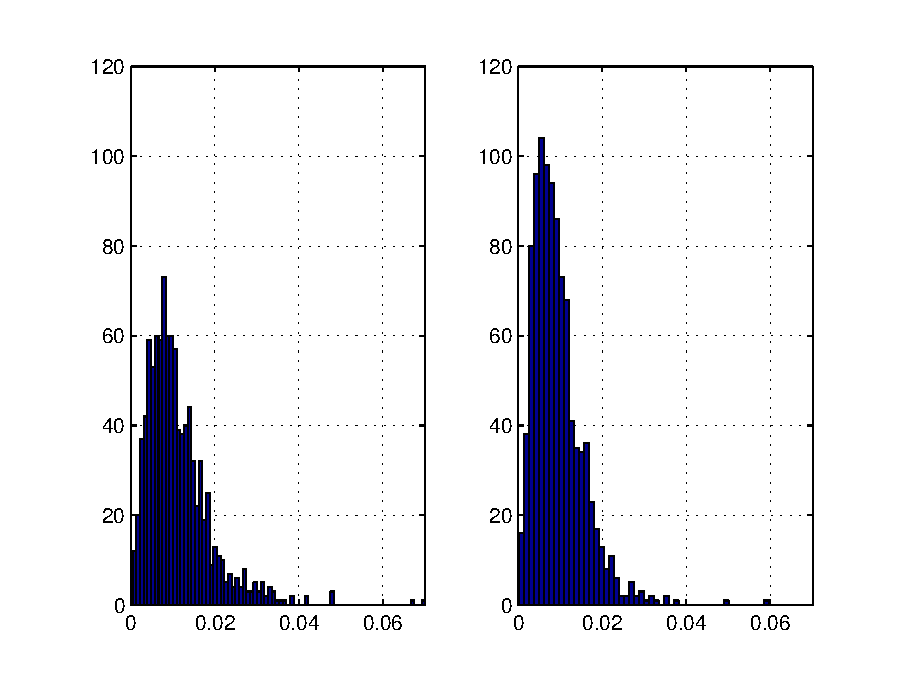
\includegraphics[width=1.1\textwidth,height=0.45\textheight]{figures/range_IRWLS/Noise02LeftBeckRightIrw}}
\caption{Histograms of the errors of the SR-LS (left) and IRWSR-LS (right) solutions, noise $\protect\sigma = 10^{-2}$}
\label{fig:Noise02IRW}
\end{figure}

\begin{figure}%[t]
\centering
  \makebox[\textwidth][c]{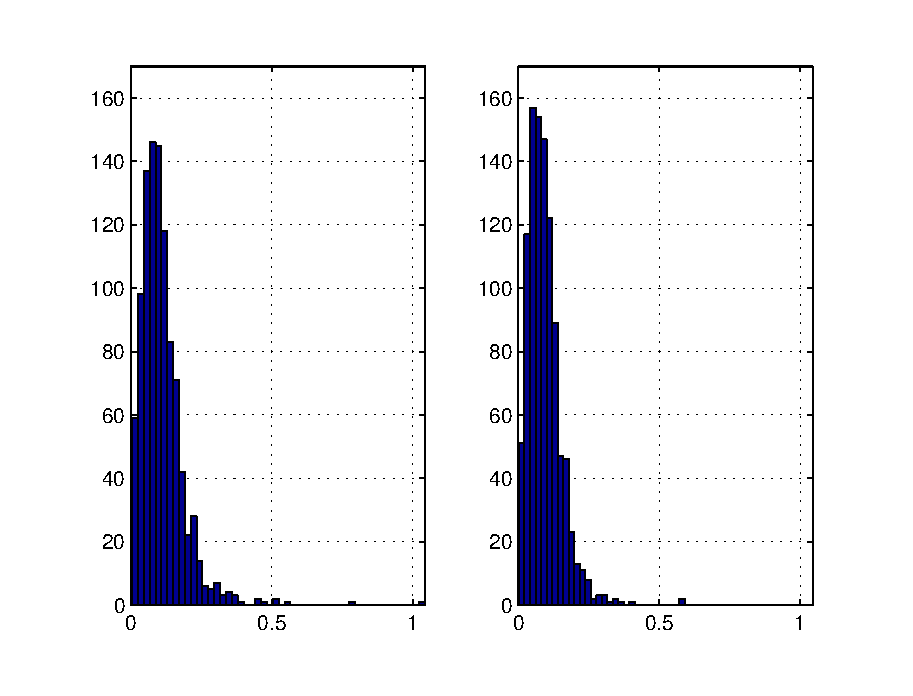
\includegraphics[width=1.1\textwidth,height=0.4\textheight]{figures/range_IRWLS/Noise01LeftBeckRightIrw}}
\caption{Histograms of the errors of the SR-LS (left) and IRWSR-LS (right) solutions, noise $\protect\sigma = 10^{-1}$}
\label{fig:Noise01IRW}
\end{figure}

\begin{figure}%[t]
\centering
  \makebox[\textwidth][c]{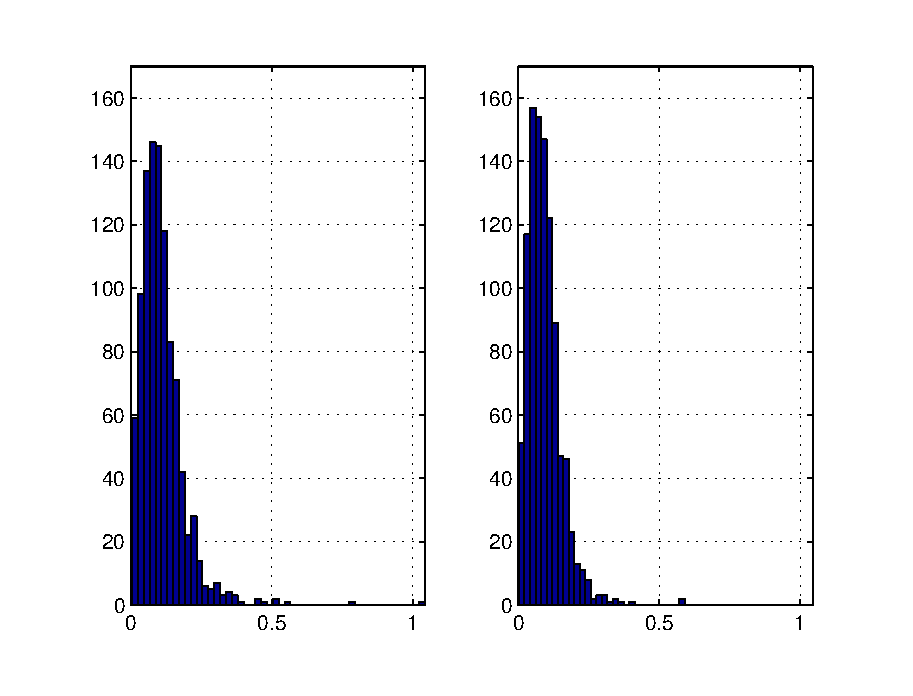
\includegraphics[width=1.1\textwidth,height=0.4\textheight]{figures/range_IRWLS/Noise01LeftBeckRightIrw}}
\caption{Histograms of the errors of the SR-LS (left) and IRWSR-LS (right) solutions, noise $\protect\sigma = 1$}
\label{fig:Noise00IRW}
\end{figure}

\newpage

\section{Source Localization From Range-Difference Measurements}%3
\subsection{Problem Formulation} %3.1

Another type of source localization problem that has attracted considerable attention is that of localizing a radiating source using range-difference measurements \cite{ StLi, BeckStLi}. In practice, range-difference measurements may be obtained from the time differences of arrival measured by an array of passive sensors. Time difference of arrival (TDOA) is a time-based positioning method based on the idea that the location of an active mobile unit (source of the signal)  can be determined by examining the difference in time at which the signal arrives at multiple reference points. 
Adopting this technique is useful in practical scenarios where synchronization between mobile units is not available \cite{GeoLoc}. Typical example of such setup includes the observed time difference of arrival (O-TDOA) technique used in 3G (WCDMA) and LTE networks to estimate the location of mobile units. In WCDMA networks only the base stations are synchronized with each other, but the mobile unit is unsynchronized with base stations. 

Each TDOA measurement constrains the location of the signal source
%mobile device 
to be on a hyperboloid with a constant range-difference between the two reference points. A TDOA measurement between base stations $BS_i$ and $BS_0$ can be given by 
\begin{equation}
\nonumber
t_{i0} = (t_i - t_x) - (t_0 - t_x) = t_i - t_0
\end{equation}
where $t_x$ is the clock time of the mobile unit, $t_i$ and $t_0$ are the time of arrival between the mobile unit and  stations $BS_i$ and $BS_0$ respectively. The equation can be written in terms of distance (range-difference) through scaling 
\begin{equation}
\nonumber
r_{i} =(t_i - t_0)c = r_i - r_0 = \|\Ba_i - \Bx\| - \|\Ba_0 - \Bx\|, i = 1,\ldots,m
\end{equation}
where $c$ is the speed of signal propagation, $r_i$ is the distance from station $\Ba_i$ to source $\Bx$, $r_0$ is the distance from station $\Ba_0$ to source $\Bx$, and $\Ba_i \in R^n$, $n = 2$ or $3$, contains coordinates of the $i$th base station.  Without loss of generality, the latter equation is valid with the assumption that the station $BS_0$ is placed at the origin of the coordinate system, i.e. $\Ba_0 = \BO$  and used as a \textit{reference} station \cite{GeoLoc}. 
%\cite{Liu} The idea of TDOA is to determine the relative position of the mobile transmitter by examining the difference in time at which the signal arrives at multiple measuring units, rather than the absolute arrival time. 
 
%obtained by comparing the signal as it is received at the $m+1$ sensors taken in pairs. 
%As usual, these sensors are denoted as $\{\Ba_0, \Ba_1,\ldots,\Ba_m\} \in R^n$ with $\Ba_0 = \BO$ be placed at the origin and used as a \textit{reference sensor}. The range-difference $r_i$ is defined as the difference between the distance from sensor $\Ba_i$ to source $\Bx$ and the distance from sensor $\Ba_0$ to source $\Bx$, namely %The range-difference measurements are obtained as

% \begin{equation} \label{eq:3.21}
% r_i=\|\Bx-\Ba_i\|-\|\Bx-\Ba_0\|=\|\Bx-\Ba_i\|-\|\Bx\|, i = 1,\ldots,m
% \end{equation}
The localization problem here is to estimate the location of a radiating source $\Bx$ given the locations of the $m+1$ sensors $\{\Ba_i, i = 0, 1, \ldots, m\}$ and noise-contaminated range-difference measurements $\{d_i, i = 1, 2, \ldots, m\}$ where 
\begin{equation} \label{eq:3.21}
d_i = r_i + \varepsilon_i = \|\Ba_i - \Bx\| - \|\Bx\| + \varepsilon_i, \mbox{ for } i = 1, 2, \ldots, m
\end{equation}
%based on measurements $d_i$'s. 
Therefore, the standard range-difference LS (RD-LS) problem is formulated as
 \begin{equation} \label{eq:3.22}
\Min_{\Bx \in R^n} F(\Bx)=\sum_{i=1}^m \left(d_i+\|\Bx\|-\|\Bx-\Ba_i\|\right)^2
 \end{equation}
 Unfortunately, finding the global solution of (\ref{eq:3.22}) turns out to be a very hard problem. Nonlinear least squares (NLLS) algorithm  \cite{{KimLeJe}} is widely used in TDOA localization systems for its performance. If  the range  measurement  errors  can  be  modeled  as  an  additive white  Gaussian  noise,  the  accuracy  of  NLLS approaches  the Cram$\acute{e}$r-Rao  lower  bound  (CRLB). However, NLLS is not guaranteed to converge  \cite{Chan}, \cite{KimLeJe} if the initial position is chosen far away from the actual source location. This becomes a more serious problem when the system coverage area is large since it becomes more difficult to fix one initial position that is close enough to the \textit{unknown} source location. Scaling by  MAjorizing  a  COmplicated  Function  (SMACOF)  strategy \cite{SMAC} can also be applied for position estimation. Compared with NLLS, it is not sensitive to the choice of the initial position and the mean-square error is guaranteed to decrease at each iteration, but  it  converges significantly slower.	
%{
%The proposed algorithm does not converge as fast as the NLLS algorithm, but it is not sensitive to the choice of
%the initial position, and the mean-square error is guaranteed to decrease at each iteration. More importantly, it does not
%require redundant receivers; when redundancy in the range measurements is unavailable, it can be used to provide the
%initial target position estimate for the NLLS algorithm. 
%Compared with  NLLS,  SMACOF  is  much  more  stable  but  it  converges significantly slower. When the number of anchors is large, both the  NLLS  and  SMACOF  methods  become  very  complex  to implement.  
%} 
%\textit{
%cite(fusion paper) Different aspects of positioning using passive ranging mea-
%surements have already been analyzed in the literature. Closed form solutions for hyperbolic positioning can be found for instance in [9]–[11]. Iterative algorithms for solving a nonlinear (weighted) least squares (N(W)LS) form another major group.
%The Gauss-Newton algorithm is studied in [12], constrained and non-constrained NLS solutions are discussed in [13], [14].
%The iterative approaches generally require good initialization to converge to the global optimum of the cost function and
%often many iterations. In order to avoid these issues, the solutions proposed in [15], [16] transform nonlinear equations into a set of linear ones, thus making real-time implementations possible. Factor graph-based methods carrying low-complex
%flags also attracted some attention [17], [18].
%......
%(cite NLOS mitigation)
%General nonlinear solutions are Maximum Likelihood (ML), Nonlinear Least Squares (NLS) or the Weighted Nonlinear Squares (WNLS) approach [5]. The WNLS solution
%requires minimization of a cost function, and performing ML estimation requires noise statistics. When the measurement
%noise n in (1) is zero-mean and Gaussian distributed with covariance matrix C n , ML scheme reduces to the WNLS solution.
%The ML approach requires a high complexity when grid search is performed, and therefore global solution may not
%be guaranteed, but in general its accuracy is the highest, especially when C n is also a function of subscriber position [6]. However, having a perfect error statistical characterization is
%difficult and others approaches are preferred. On the other hand, NLS does not require noise statistics but also involves
%the same issues as ML.
%} 
Reference \cite{BeckStLi} proposes a squared range-difference LS (SRD-LS) approach to address this problem, which is summarized below.

 By writing (\ref{eq:3.21}) as $d_i+\|\Bx\|=\|\Bx-\Ba_i\|$ and squaring both sides, we obtain
  \begin{equation} \label{eq:3.23}
\left(d_i+\|\Bx\|\right)^2 = \|\Bx-\Ba_i\|^2
 \end{equation}
 which can be simplified to
  \begin{equation} \label{eq:3.24}
-2d_i\|\Bx\|-2\Ba_i^T\Bx=g_i, i=1,\ldots,m
 \end{equation}
 where $g_i=d_i^2-\|\Ba_i\|^2$. In practice (\ref{eq:3.24}) does not hold exactly due to measurement noise that contaminates the data $d_i$'s. In other words, if $d_i$'s in (\ref{eq:3.24}) are taken to be real-world data, then we only have
 \begin{equation} \label{eq:3.25}
-2d_i\|\Bx\|-2\Ba_i^T\Bx-g_i\approx 0, i=1,\ldots,m
 \end{equation}
 Reference \cite{BeckStLi} proposes a LS solution for the problem at hand by minimizing the sum of squared residues on the left side of (\ref{eq:3.25}), namely,
 \begin{equation}\label{eq:3.26}
\Min_{{\Bx} \in R^{n}} \sum_{i=1}^m \left(-2\Ba_i^T\Bx-2d_i\|\Bx\|-g_i\right)^2
\end{equation}
 By introducing new variable $\By=[\Bx^T \|\Bx\|]^T$ and noticing nonnegativity of the component $y_{n+1}$ problem (\ref{eq:3.26}) is converted to
 \begin{eqnarray}\label{eq:3.27}%40
\setcounter{abc}{1}
\Min_{\By\in R^{n+1}} \|\BB\By-\Bg\|^2 \\
\stepcounter{abc} \setcounter{equation}{27}
\mbox{subject to: } \By^T\BC\By = 0 \\
\stepcounter{abc} \setcounter{equation}{27}
y_{n+1}\geq 0
\end{eqnarray}
where $\Bg=[g_1 \ldots g_m]^T$ and
\begin{equation}
\nonumber
\setcounter{abc}{0}
%\label{eq:3.28} %41
\setcounter{abc}{0}
\BB = \left(\begin{array}{cc}
    -2\Ba_1^T & -2d_1 \\
    \vdots & \vdots \\
    -2\Ba_m^T & -2d_m
    \end{array}\right),
\BC =  \left(\begin{array}{cc}
    \BI_n & \BO_{n \times 1} \\
    \BO_{1 \times n} & -1
    \end{array}\right)
\end{equation}
Because of the presence of the nonnegativity constraint in (\ref{eq:3.27}c), (\ref{eq:3.27}) is no longer a GTRS problem hence the technique used for the case of range measurements does not apply. Nevertheless reference \cite{BeckStLi} presents a rigorous argument which shows that the optimal solution of (\ref{eq:3.27}) either assumes the form of
 \begin{equation}\label{eq:3.28}
 %\nonumber
 \tilde{\By}(\lambda)=\left(\BB^T\BB+\lambda\BC\right)^{-1}\BB^T\Bg
 \end{equation}
 where $\lambda$ solves
 \begin{equation}\label{eq:3.29}
 \tilde{\By}(\lambda)^T\BC\tilde{\By}(\lambda)=0
 \end{equation}
 and makes $\BB^T\BB+\lambda\BC$ positive definite, or is the vector among $\{\BO,$ $\tilde{\By}(\lambda_1),\ldots,\tilde{\By}(\lambda_p)\}$ that gives the smallest objective function in (\ref{eq:3.27}a), where $\{\lambda_i, i = 1,\ldots,p\}$ are all roots of (\ref{eq:3.29}) such that the $(n+1)$'th component of $\tilde{\By}(\lambda_i)$ is nonnegative and $\BB^T\BB+\lambda\BC$ has exactly one negative and $n$ positive eigenvalues. We shall refer the global solution of (\ref{eq:3.27}) to as the SRD-LS solution.

\subsection{Improved Solution Using Iterative Re-weighting} %3.2
%\subsubsection{Weighted squared range-difference based least squares solution}
\subsubsection{The Algorithm} %3.2.1

We now present a method for improved solutions over SRD-LS solutions. The method incorporates an iterative re-weighting procedure into the SRD-LS approach, hence it is in spirit similar to the IRWRS-LS approach described in Sec. \ref{chapter:irw}.1.2. We begin by considering the weighted SRD-LS problem
\begin{equation} \label{eq:3.30}
\Min_{{\Bx} \in R^n} \sum_{i=1}^m w_i\left(-2\Ba_i^T\Bx-2d_i\|\Bx\|-g_i\right)^2
\end{equation}
where weights $w_i$ for $i=1,\ldots,m$ are fixed nonnegative constants. The counterpart of (\ref{eq:3.28}) for the problem (\ref{eq:3.30}) is given by
\begin{eqnarray} \label{eq:3.31}
\setcounter{abc}{1}
\Min_{\By \in R^{n+1}} \|\BB_w\By - \Bg_w\| \\
\stepcounter{abc} \setcounter{equation}{31}
\mbox{subject to: } \By^T\BC\By = 0 \\
\stepcounter{abc} \setcounter{equation}{31}
y_{n+1}\geq 0
\end{eqnarray}
where $\BB_w=\BGA\BB$, $\Bg_w=\BGA\Bg$ and $\BGA=\mbox{diag}\{\sqrt{w_1},\ldots,\sqrt{w_m}\}$, which will be referred to as the weighted SRD-LS (WSRD-LS) problem. On comparing (\ref{eq:3.31}) with (\ref{eq:3.28}), it follows immediately that the global solver for problem (\ref{eq:3.28}) characterized by data set $\{\BB, \Bg, \BC\}$ can also be sued for solving problem (\ref{eq:3.31}) be used applying it to data set $\{\BB_w, \Bg_w, \BC\}$.

Concerning the assignment of weights $\{w_i, i=1,\ldots,w_m\}$, we recall (\ref{eq:3.23}), (\ref{eq:3.24}) and observe that the $i$th term of the objective function in (\ref{eq:3.30}) can be written as
\begin{equation} \label{w:srd}
\nonumber
\begin{aligned}
&w_i\left(-2d_i\|\Bx\|-2\Ba_i^T\Bx-g_i\right)^2 \\
=&w_i\left((d_i+\|\Bx\|)^2-\|\Bx-\Ba_i\|^2\right)^2 \\
=&w_i\left(d_i+\|\Bx\|+\|\Bx-\Ba_i\|\right)\left(d_i+\|\Bx\|-\|\Bx-\Ba_i\|\right)
\end{aligned}
\end{equation}
Clearly, the last expression above would become the $i$th term of the objective function in the RD-LS problem (\ref{eq:3.22}) if weights $w_i$ were set to
\begin{equation}
\nonumber
 \frac{1}{\left(d_i+\|\Bx\|+\|\Bx-\Ba_i\|\right)^2}
\end{equation} 
so that the first two factors are cancelled out. This suggests that a realizable weight assignment for performing practically the same cancellation can be made by means of iterative re-weighting for problems (\ref{eq:3.30}) and (\ref{eq:3.31}) where the weights in the $k$th iteration are assigned to
\begin{equation} \label{eq:3.32}
\setcounter{abc}{0}
w_i^{(k)}=\frac{1}{\left(d_i+\|\Bx_{k-1}\|+\|\Bx_{k-1}-\Ba_i\|\right)^2}, i=1,\ldots,m
\end{equation}

Based on the analysis above, a localization algorithm for range-difference measurements can be outlined as follows.

%\begin{table} \label{alg:rd-ls}
%\centering
%\caption{Iterative re-weighting least-squares method for source localization based on range-difference measurements.}
%\begin{tabular}{|l|l|} \hline
%\centering
%. & \textbf{Algorithm 3.2} \\ \hline
%%&&& \\ 
%\textbf{Input} &	Sensor locations $\{\Ba_i, i=0, 1,\ldots,m\}$ with $\Ba_0=\BO$, range-difference measurements $\{d_i, i = 1,\ldots,m\}$, maximum number of iterations $k_{max}$, convergence tolerance $\xi$.	
%\\ &\\ \hline
%\textbf{Output} & $\protect\Bx^*$ \\ & \\ \hline
%\textbf{Step 1} & Generate data set $\{\BB, \Bg, \BC\}$ as 
%$\Bg = \left(\begin{array}{c}
%    d_1^2 - \|\Ba_1\|^2 \\
%    \vdots \\
%    d_m^2 - \|\Ba_m\|^2
%    \end{array}\right), 
%\BB = \left(\begin{array}{cc}
%    -2\Ba_1^T & -2d_1 \\
%    \vdots & \vdots \\
%    -2\Ba_m^T & -2d_m
%    \end{array}\right),
%\BC =  \left(\begin{array}{cc}
%    \BI_n & \BO_{n \times 1} \\
%    \BO_{1 \times n} & -1
%   \end{array}\right).
%$
%Set $k=1$, $w_i^{(1)}=1$ for $i=1,\ldots,m$.
%\\ &\\ \hline
%\textbf{Step 2} &	 Set $\BGA_k=\mbox{diag}\left(\sqrt{w_1^{(k)}},\ldots,\sqrt{w_m^{(k)}}\right)$, $\BB_w=\BGA_k\BB$ and $\Bg_w=\BGA_k\Bg$.
%\\ &\\ \hline
%\textbf{Step 3} & Solve WSRD-LS problem
%$\Min_{\By \in R^{n+1}} \|\BB_w\By - \Bg_w\|$
%$ \mbox{subject to: } \By^T\BC\By = 0 $
%$y_{n+1}\geq 0$
%to obtain its global solution $\Bx_k$.	
%\\& \\ \hline
%\textbf{Step 4} & If $k=k_{max}$ or $\|\Bx_k-\Bx_{k-1}\|<\xi$, terminate and output $\Bx_k$ as the solution; otherwise, set $k=k+1$, update weights $\{w_i^{(k)}, i=1,\ldots,m\}$ as 
%$ w_i^{(k)}=\frac{1}{\left(d_i+\|\Bx_{k-1}\|+\|\Bx_{k-1}-\Ba_i\|\right)^2} $
%and repeat from Step 2.
%\\ %&&&&\\
%\hline
%\end{tabular}
%\end{table}

\phantom{m}
\framebox{%
\parbox{5.5in}{
\textbf{Algorithm 2} 

1) Input data: Sensor locations $\{\Ba_i, i=0, 1,\ldots,m\}$ with $\Ba_0=\BO$, range-difference measurements $\{d_i, i = 1,\ldots,m\}$, maximum number of iterations $k_{max}$ and convergence tolerance $\xi$.

2) Generate data set $\{\BB, \Bg, \BC\}$ as
\begin{equation} 
\nonumber
\setcounter{abc}{0}
\Bg = \left(\begin{array}{c}
    d_1^2 - \|\Ba_1\|^2 \\
    \vdots \\
    d_m^2 - \|\Ba_m\|^2
    \end{array}\right),
\BB = \left(\begin{array}{cc}
    -2\Ba_1^T & -2d_1 \\
    \vdots & \vdots \\
    -2\Ba_m^T & -2d_m
    \end{array}\right),
\BC =  \left(\begin{array}{cc}
    \BI_n & \BO_{n \times 1} \\
    \BO_{1 \times n} & -1
    \end{array}\right).
\end{equation}
Set $k=1$, $w_i^{(1)}=1$ for $i=1,\ldots,m$.

3) Set $\BGA_k=\mbox{diag}\left(\sqrt{w_1^{(k)}},\ldots,\sqrt{w_m^{(k)}}\right)$, $\BB_w=\BGA_k\BB$ and $\Bg_w=\BGA_k\Bg$.

4) Solve WSRD-LS problem
\begin{eqnarray}
\nonumber
\Min_{\By \in R^{n+1}} \|\BB_w\By - \Bg_w\| \\
\nonumber
\mbox{subject to: } \By^T\BC\By = 0 \\
\nonumber
y_{n+1}\geq 0
\end{eqnarray}
to obtain its global solution $\Bx_k$.

5) If $k=k_{max}$ or $\|\Bx_k-\Bx_{k-1}\|<\xi$, terminate and output $\Bx_k$ as the solution; otherwise, set $k=k+1$, update weights $\{w_i^{(k)}, i=1,\ldots,m\}$ as 
\begin{equation}
\nonumber
\setcounter{abc}{0}
w_i^{(k)}=\frac{1}{\left(d_i+\|\Bx_{k-1}\|+\|\Bx_{k-1}-\Ba_i\|\right)^2}
\end{equation}
and repeat from Step 3).
}
} \label{alg:rd-ls}

\phantom{m}

It is evident that the complexity of the algorithm is practically equal to the complexity of the WSRD-LS solver involved in Step 4 times the number of iterations, $k$, which is typically in the range of 3 to 6. We shall call the solutions obtained from Algorithm 2 IRWSRD-LS solutions. Technical details on how to solve (\ref{eq:3.31}) can be found in Appendix 1.


\subsubsection{A variant of Algorithm 2}

Like in the case of range measurements, once the IRWSRD-LS solution is obtained by applying Algorithm 2, which is expected to be within a small vicinity of the true global solution of the RD-LS problem (\ref{eq:3.22}), the gap can be closed by running a good local method that takes the IRWSRD-LS solution as an initial point. Again, the Newton method is chosen for its fast convergence, low complexity due to the extremely low dimension $n$, and the availability of closed-form formulas to compute the gradient and Hessian of $F(\Bx)$ in (\ref{eq:3.22}).

Assuming $\Bx\neq\Ba_i$ for $i = 0, 1,\ldots, m$, the gradient and Hessian of $F(\Bx)$ is found to be
\begin{equation}
\nonumber
\Bg(\Bx)=\sum_{i=1}^m c_i\left(\Bq_i - \tilde(\Bx)\right)
\end{equation}
and
\begin{equation}
\nonumber
\BH(\Bx)=\sum_{i=1}^m \left[(\Bq_i-\tilde(\Bx))(\Bq_i-\tilde(\Bx))^T+c_i(\BQ_{1i}+\BQ_2)\right]
\end{equation}
respectively, where
\begin{equation}
\nonumber
c_i=\|\Bx-\Ba_i\|-\|\Bx\|, \Bq_i=\frac{\Bx-\Ba_i}{\|\Bx-\Ba_i\|}, \tilde{\Bx}=\frac{\Bx}{\|\Bx\|}
\end{equation}
and
\begin{equation}
\nonumber
\BQ_{1i}=\frac{1}{\|\Bx-\Ba_i\|}\left(\BI-\Bq_i\Bq^T\right), \BQ_2=\frac{1}{\|\Bx\|}\left(\BI-\tilde{\Bx}\tilde{\Bx}^T\right)
\end{equation}
To ensure the positive definiteness of Hessian, eigen decomposition of $\BH(\Bx)$, namely,
\begin{equation}
\nonumber
\BH(\Bx)=\BU\BLA\BU^T
\end{equation}
may be performed, where $\BU$ is orthogonal and $\BLA=\mbox{diag}(\lambda_1,$ $\ldots,\lambda_n)$ with $\{\lambda_i, i=1,\ldots,n\}$ being the eigenvalues of $\BH(\Bx)$. Let $\lambda_{min}$ be the smallest eigenvalue of $\BH(\Bx)$. If $\lambda_{min}$, then $\BH(\Bx)$ is positive definite and the Newton algorithm is carried out without modification; if $\lambda_{min}\leq0$, then the algorithm uses a slightly modified Hessian given by
\begin{equation}
\nonumber
\tilde{\BH}(\Bx)=\BU\tilde{\BLA}\BU^T
\end{equation}
where $\tilde{\BLA}=\mbox{diag}\left(\tilde{\lambda}_1,\ldots,\tilde{\lambda}_n\right)$ with
\begin{equation}
\nonumber
\tilde{\lambda}_i=\left\{\begin{array} {lll}
    \lambda_i & \mbox{if } \lambda_i>0 & \\
    \delta &  \mbox{if } \lambda_i\leq0 & i=1,\ldots,m \end{array} \right.
\end{equation}
and $\delta$ a small positive constant. Obviously, $\tilde{\BH}(\Bx)$ is guaranteed to be positive definite. In what follows, solutions obtained by the proposed two-step method are called \textit{hybrid} IRWSRD-LS solutions.

\subsection{Numerical Results}


Performance of the proposed algorithms was evaluated and compared with the method of  \cite{BeckStLi} by Monte Carlo simulations with a set-up similar to that of \cite{BeckStLi}. SRD-LS solutions were used as performance benchmarks for Algorithm 2 and its variant. In both cases the system consisted of m sensors $\{\Ba_i, i=1, 2,\ldots,m\}$ randomly placed in the planar region in $R^2$, and a radiating source $\Bx_s$, located randomly in the region $\{\Bx=[x_1;x_2], -10\leq x_1,x_2\leq 10\}$. The coordinates of the source and sensors were generated for each dimension following a uniform distribution. Measurement noise $\{\varepsilon_i, i=1,\ldots,m\}$ was modelled as independent and identically distributed (i.i.d) random variables with zero mean and variance $\sigma^2$. Accuracy of source location estimation was evaluated in terms of mean squared error in the form $\mbox{MSE} = E\{\|\Bx^*-\Bx_s\|\}$ where $\Bx_s$ denotes the exact source location and $\Bx^*$ is its estimation obtained by SRD-LS, IRWSRD-LS and \textit{hybrid} IRWSRD-LS methods, respectively. Table \ref{tab:3} provides comparisons of these methods with SRD-LS, where each entry was averaged MSE over 1,000 Monte Carlo runs of the method. For the columns representing performance of the IRWSDR-LS and \textit{hybrid} IRWSDR-LS methods each table entry lists their MSE and relative improvement over SRD-LS solutions in percentage, in the format: MSE($\%$ Improvement).

\begin{table}[h]
\centering
\caption{MSE of position estimation for SRD-LS, IRWSRD-LS and \textit{hybrid} IRWSRD-LS methods}
\begin{tabular}{|c|c|c|c|} \hline
\centering
$\sigma$ & SR - LS & IRWSR-LS (Im.,\%) & \textit{hybrid} IRWSR-LS (Im.,\%) \\ \hline
%&&& \\
1e-04& 1.3830e-08  & 8.2271e-09 (40) &  8.2270e-09 (40) \\ &&&\\ 
1e-03&	1.3063e-06  & 8.2828e-07 (37)&  8.2827e-07 (37) \\ &&&\\
1e-02&	1.1163e-04  & 6.6779e-05 (40)&  6.6779e-05 (40)  \\ &&&\\
1e-01&	1.2095e-02  & 7.2089e-03 (40)&  7.2089e-03 (40) 	 \\ &&&\\
1e+0&	1.5705e+00  & 9.7075e-01 (38)&  9.7075e-01 (38)  \\ %&&&&\\
\hline
\end{tabular}
\label{tab:3}
%\end{table}

%\begin{table}
%\centering
\caption{Standard deviation of the squared estimation error for SRD-LS, IRWSRD-LS and \textit{hybrid} IRWSRD-LS methods}
\begin{tabular}{|c|c|c|c|} \hline
$\sigma$ & SR - LS & IRWSR-LS & \textit{hybrid} IRWSR-LS \\ \hline
%&&& \\ 
1e-04&  4.5624e-08 &   2.2446e-08 &  2.2446e-08\\ &&&\\
1e-03&	3.9506e-06 &   3.1610e-06 &  3.1610e-06\\ &&&\\
1e-02&	2.2710e-04 &   1.2812e-04 &  1.2812e-04\\ &&&\\
1e-01&	3.0108e-02 &   1.8891e-02 &  1.8891e-02\\ &&&\\
1e+0&	4.5781e+00 &   3.0597e+00 &  3.0597e+00\\ %&&&&\\
\hline
\end{tabular}
\label{tab:4}
\end{table}

The simulation studies of Algorithm 2 considered $m = 11$ sensors $\{\Ba_i, i=1, 2,\ldots,10\}$ with $\Ba_0=\BO$ and other ten sensors placed in the region $[-15;15]\times[-15;15]$, with $\sigma$ being one of five possible levels $\{10^{-4}, 10^{-3}, 10^{-2}, 10^{-1}, 1\}$. The range-difference measurements used to form  matrix $\BB$ in Step 2 of the Algorithm 2 were calculated as a noise-contaminated range-difference measurements $d_i$ in (\ref{eq:3.21}).% as:
%\begin{equation}
%\nonumber
%d^{noisy}_i = d_i + \varepsilon_i.
%\end{equation}
Step 4 of Algorithm 2 was carried out using the SRD-LS algorithm in \cite{BeckStLi}. Again, the IRWSRD-LS solutions offer considerable improvement over SRD-LS solutions. Further analysis of the data that was used to generate Table \ref{tab:3} illustrates the advantage of the IRWSR-LS (hybrid IRWSR-LS) solution over the SR-LS.

Each entry in Table \ref{tab:4} is a standard deviation of the squared  estimation errors  aggregated over the  same 1,000 Monte Carlo runs described above in Table \ref{tab:3} (where the MSE of the position estimation are shown). The results summarised in Table \ref{tab:4} suggest that, again, IRWSR-LS and hybrid IRWSR-LS outperform SR-LS. Figures (\ref{fig:Noise04IRDW} - \ref{fig:Noise00IRDW}) describe the histograms of the location estimation errors $\|\Bx^* - \Bx_s\|$ of the SR-LS solution (left images) and IRWSR-LS (right images) for all four noise levels with $\sigma$ being one of $\{10^{-3}, 10^{-2}, 10^{-1}, 1\}$. Here $\Bx^*$ denotes the estimated location and $\Bx_s$ is the exact location of the source. Histograms that correspond to the results obtained by IRWSR-LS are shifted closer towards $0$ than those obtained by SR-LS, have smaller variance, and in most cases have fewer outliers with large error.



\begin{figure}[h]
\centering
  \makebox[\textwidth][c]{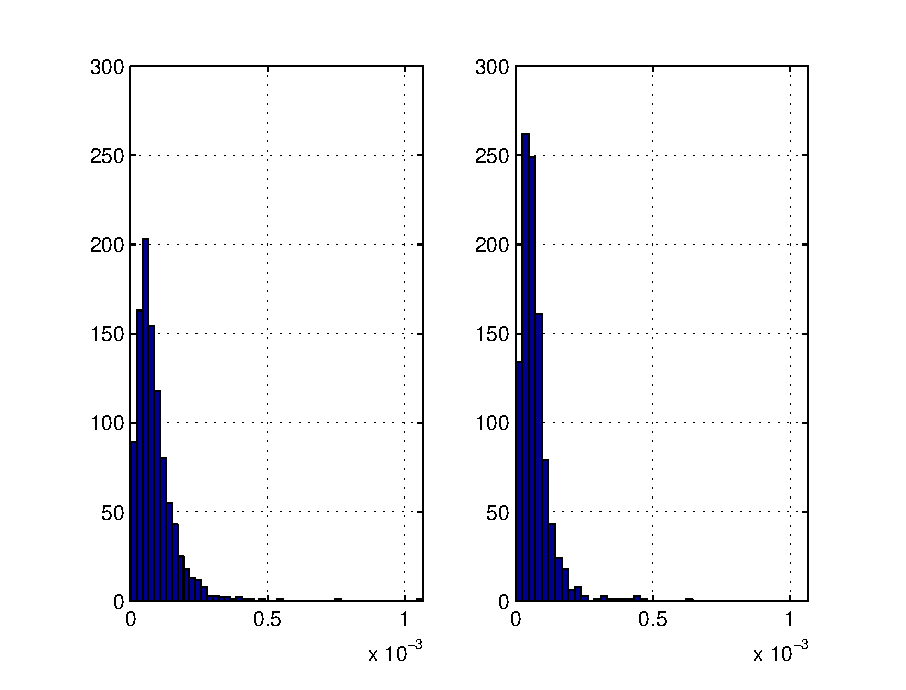
\includegraphics[width=1\textwidth,height=0.42\textheight]{figures/range_dif_IRWLS/Noise04LeftBeckRightRD}}
\caption{Histograms of the errors of the SR-LS (left) and IRWSR-LS (right) solutions, noise $\protect\sigma = 10^{-4}$}
\label{fig:Noise04IRDW}
\end{figure}

\begin{figure}%[t]
\centering
  \makebox[\textwidth][c]{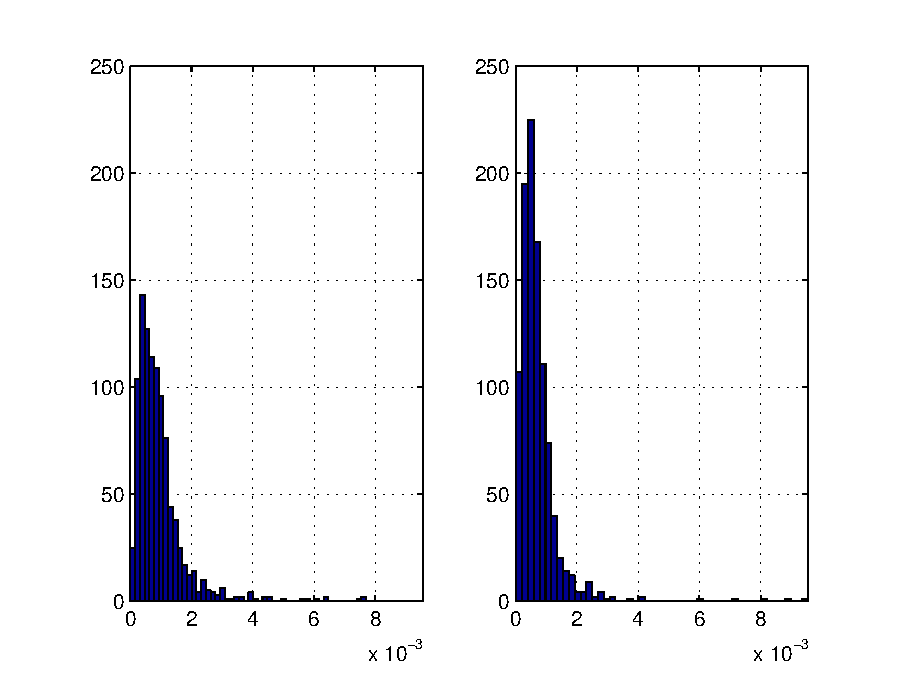
\includegraphics[width=1\textwidth,height=0.42\textheight]{figures/range_dif_IRWLS/Noise03LeftBeckRightRD}}
\caption{Histograms of the errors of the SR-LS (left) and IRWSR-LS (right) solutions, noise $\protect\sigma = 10^{-3}$}
\label{fig:Noise03IRDW}
\end{figure}

\begin{figure}%[t]
\centering
  \makebox[\textwidth][c]{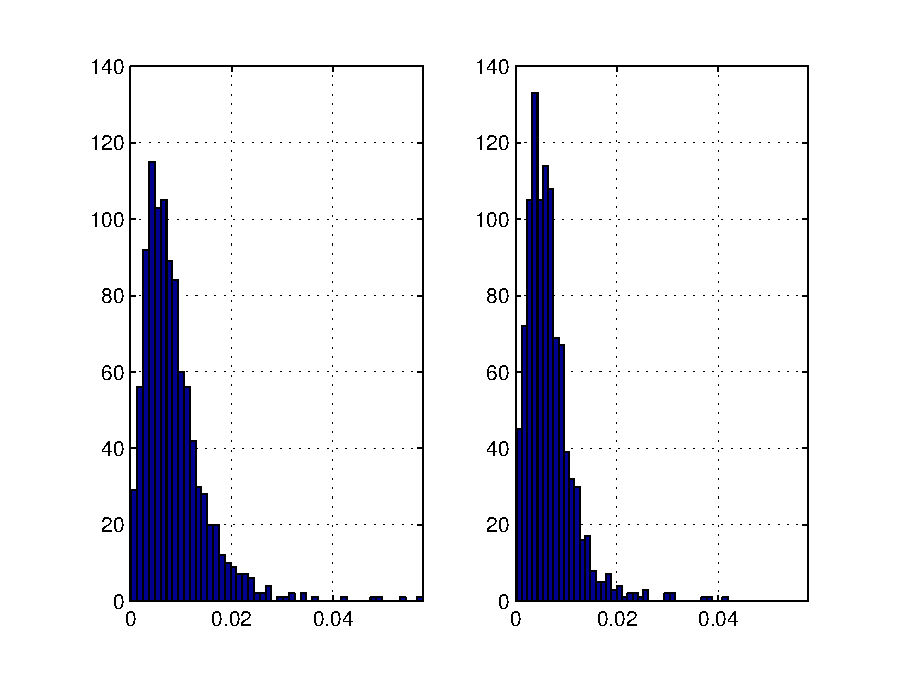
\includegraphics[width=1\textwidth,height=0.42\textheight]{figures/range_dif_IRWLS/Noise02LeftBeckRightRD}}
\caption{Histograms of the errors of the SR-LS (left) and IRWSR-LS (right) solutions, noise $\protect\sigma = 10^{-2}$}
\label{fig:Noise02IRDW}
\end{figure}

\begin{figure}%[t]
\centering
  \makebox[\textwidth][c]{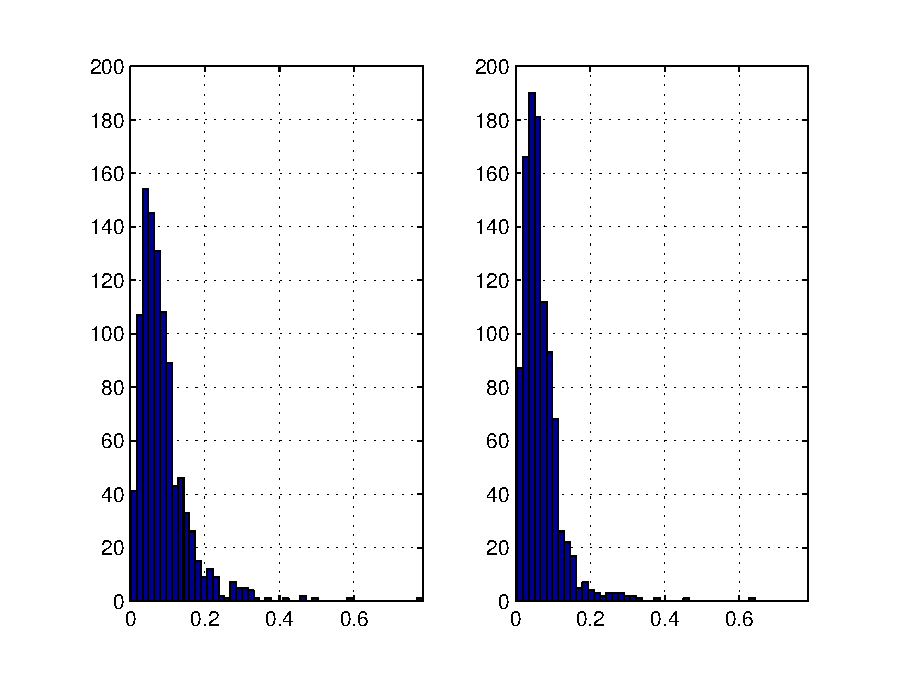
\includegraphics[width=1\textwidth,height=0.42\textheight]{figures/range_dif_IRWLS/Noise01LeftBeckRightRD}}
\caption{Histograms of the errors of the SR-LS (left) and IRWSR-LS (right) solutions, noise $\protect\sigma = 10^{-1}$}
\label{fig:Noise01IRDW}
\end{figure}

\begin{figure}%[t]
\centering
  \makebox[\textwidth][c]{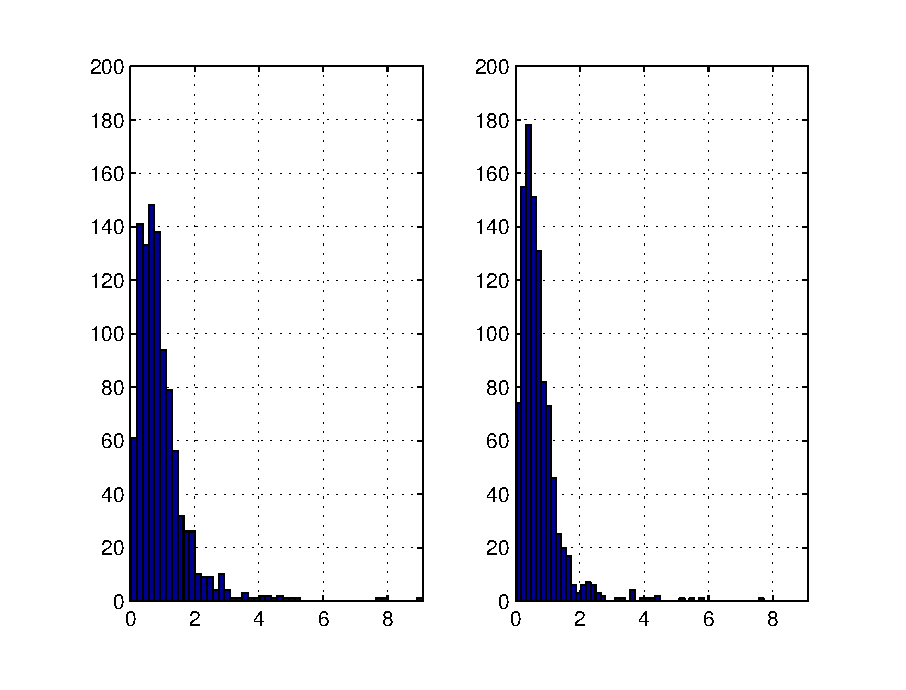
\includegraphics[width=1\textwidth,height=0.42\textheight]{figures/range_dif_IRWLS/Noise00LeftBeckRightRD}}
\caption{Histograms of the errors of the SR-LS (left) and IRWSR-LS (right) solutions, noise $\protect\sigma = 1$}
\label{fig:Noise00IRDW}
\end{figure}



\newpage
\section{Extensions}


Methods developed in this chapter for localization based on range measurements can be adopted to solve the problem of signle sourse localization from energy measurements \cite{StLi}. 
% \cite{LiHu,ShengHu,Saric} \cite{LuWuYan}
%The energy, acoustic or RF, of the signal received by the sensor is inversely proportional to the distance between sensor and the radiating source (\cite{LiHu,ShengHu,Saric}).
%The localization based on the received signal strength uses the property that sound energy attenuates with the square of the distance from the source \cite{Saric}.
Energy-based source localization, advocated in \cite{LiHu}, \cite{Saric}, is motivated by a simple observation that the sound level decreases when the distance between sound source and the listener becomes large. By modeling the relation between sound level (energy) and distance from the sound source, one may estimate the source location using multiple energy readings at different known sensor locations. When the sound is propagating through the air, it is known that the acoustic energy emitted omnidirectionally from a sound source will attenuate at a rate that is inversely proportional to the square of the distance \cite{LiHu}. Using this fact and some simple manipulations, it is possible to obtain an equation in the vector of unknow source location $\Bx$ that is somewhat similar to (\ref{eq:3.9}). The rest of the section provides technical details of this reformulation. 

%(from \cite{StLi}) "The source localization problem from range measurements is related to the problem of source localization from energy measurements \cite{LiHu,ShengHu,Saric}.
%The energy measurement based source localization approach, advocated in \cite{LiHu}, \cite{Saric} is based on the fact that the energy of the signal received by the $i$th sensor over a (relatively small) time interval is inversely proportional to $\| \Bx - \Ba_i \|$, for $i = 1, 2, \ldots,m$. 

%Using this fact and some simple manipulations (see, e.g., \cite{LiHu} for details), it is possible to obtain an equation in the unknown vector x that is somewhat similar to (2), namely:....."

%This section provides an example of ...
%In this section, a reformulation of the maximum liklihood source localization using acoustic energy meausrements is offered.
%Acoustic energy attenuation model presented here is based on assumptions of \cite{LiHu} and \cite{Saric} (or please refer for details). Only single sourse localization is investigated in this section.


\subsection{Acoustic Energy Attenuation Model} %and Parameter Estimator}


Let $m$ be a number of acoustic sensors. For consistency of notation, let $\Ba_i$ denote the known location of the sensor $i$ in space $R^n$, $n = 2$ or $3$. Each sensor measures the acoustic intensity radiated by a source $\Bx\in R^n$ over a time period $T = \frac{M}{f_s}$, where M is the number of sample points used for estimating the acoustic enery and $f_s$ is the sampling frequency. % (\textbf{OR} Received signal is an acoustic pulse $M$-samples wide.)
 Acoustic energy received by sensor $i$ over a time period $T$ can be represented as:
\begin{equation} \label{eq:3.33}
r_i = g_i \frac{S}{\|\Bx - \Ba_i\|^\alpha} + \varepsilon_i
\end{equation}
where $\|\Bx - \Ba_i\|$ is the Euclidean distance between the $i$th sensor and the source. $g_i$ is a factor that takes into account $i$th sensor gain. It is asssumed that the gain of individual sensors is either known, i.e. obtained at the sensor callibration stage, or is same for all sensors. $S$ is the unknown acoustic energy measured 1 unit distance away from the source. $\alpha$ is the energy decay factor %(pathloss exponent) 
and is usually assumed to have a value 2 \cite{LiHu}. $\varepsilon_i$ denotes the square of the background noise affecting the measurement of sensor $i$. Based on the central limit theorem, it can be approximated well as a normal distribution%/ It is assumed to be a wide-sense stationary Gaussian random process \cite{LiuHuPan} / 
, namely, $\varepsilon_i \sim N(\mu_i, \sigma_i^2)$ with a positive mean value $\mu_i$ that is no less that the standard deviation $\sigma_i$ that can be estimated empirically from data samples \cite{LiHu}. More details on derivation and assumptions of this model can be found in %For justification and validity of this energy attenuation model, please see 
\cite{LiHu}\cite{Saric}, \cite{LiuHuPan} and its references. %\cite{ShengHu},


References \cite{LiHu,ShengHu} argue that the maximum likelihood estimation of the vector of unknown parameters $\Btheta = [\Bx^T S]^T$ can be obtained my minimizing the quadratic form
\begin{equation} \label{eq:3.34}
\Min_\theta \quad \ell(\Btheta) = \|\BZ - S\BH\|
\end{equation}
where 
\begin{equation}
\nonumber
\BH = \left[ \begin{array}{c}
\frac{g_1}{\sigma_1\|\Bx - \Ba_1 \|^2} \\
\frac{g_2}{\sigma_2|\Bx - \Ba_2 \|^2} \\
\vdots \\
\frac{g_m}{\sigma_m|\Bx - \Ba_m \|^2} \\
\end{array}
\right] ,
\nonumber
\BZ = \left[ \begin{array}{c}
\frac{y_1 - \mu_1}{\sigma_1} \\
\frac{y_2 - \mu_2}{\sigma_2} \\
\vdots \\
\frac{y_m - \mu_m}{\sigma_m} \\
\end{array}
\right] ,
\end{equation}
and $\BZ$ are (estimated) normalized energy measurements for the case of the single radiating source. Important assumption about (\ref{eq:3.34}) is that $\mu_i$ and $\sigma_i$ are considered known. 


\subsection{Reformulation}

There are two things to note about (\ref{eq:3.34}). First, (\ref{eq:3.34}) is a \textit{nonlinear} least square objective function because the vector $\BH$ is a nonlinear function of the $n$  unknown source coordinates, where $n$ is the dimention of the location coordinates. Second, although there are $m$ sensors reporting the acousting energy reading in fact there are $n + 1 \leq m$ unknowns, including the unknown acoustic energy $S$ radiated from the source. 
To eliminate the unknown source energy $S$ \cite{ShengHu}  propose first to compute the ratio $k_{ij}$ of the calibrated energy readings from $i$th and $j$th sensor as
\begin{equation} \label{eq:3.35}
k_{ij} = \left[ \frac{z_i / g_i}{z_j / g_j} \right]^{-1/\alpha} = \frac{\|\Bx - \Ba_i\|}{\|\Bx - \Ba_j\|}
\end{equation}
for $i = 1, 2, \ldots, m-1$, and $j = i+1, \ldots, m$. For the case $0 < k_{ij} \neq 1$ all possible source coordinates $\Bx$ that form a solution to (\ref{eq:3.35}) reside on a $n$-dimensional hyper-sphere described by the equation:
\begin{equation} \label{eq:3.36}
\| \Bx - \Bc \|^2 = \rho_{ij}^2
\end{equation}
where the center $\Bc_{ij}$ and the radius $\rho_{ij}$ of the hyper-sphere associated with the sensors $i$ and $j$  are given by:
\begin{equation} \label{eq:3.37}
\Bc_{ij} = \frac{\Ba_i - k_{ij}^2\cdot\Ba_j}{1-k_{ij}^2}, \rho_{ij} = \frac{k_{ij}\|\Ba_i - \Ba_j\|}{1-k_{ij}^2}
\end{equation}
For the case when $k_{ij} \rightarrow 1$ the possible source locations $\Bx$ reside on the hyperplane between sensors $\Ba_i$ and $\Ba_j$:
\begin{equation}
\nonumber
\Bx^T \Bgamma_{ij} = \tau_{ij}
\end{equation}
where $\Bgamma_{ij} = \Ba_i - \Ba_j$ and $\tau_{ij} = (\|\Ba_i\|^2 - \|\Ba_j\|^2) / 2$. 

Let $I_1$ and $I_2$ be two index sets such that $0 < k_{ij} \neq 1$ for all $\{i, j \} \in I_1$ and $k_{ij} = 1$ for all $\{i, j\} \in I_2$ with $1 \leq i \leq m-1, i+1 \leq j \leq m $   and $I_1 \cap I_2 = \emptyset$.
Let $L_1$ and $L_2$ denote the number of elements in sets $I_1$ and $I_2$ respectively (number of hyperspheres and hyperplanes) and $L_1 + L_2 = m(m-1)/2$. Then the unknown location of the source can be found via minimization of the criterion that is equivalent to (\ref{eq:3.34}) \cite{ShengHu}:
\begin{equation} \label{eq:3.38}
%\Min \sum_{i,j \in I_1}^{} \left(\ \|\Bx - \Bc_{ij}\|^2 - \rho_{ij}^2\right)^2 + \sum_{i,j \in I_2}^{} \left( \Bx^T \Bgamma_{ij}  - \tau_{ij}\right)^2
\Min_{\Bx} \sum_{l_1 = 1}^{L_1} \left(\ \|\Bx - \Bc_{l_1}\|^2 - \rho_{l_1}^2\right)^2 + \sum_{l_2 = 1}^{L_2} \left( \Bx^T \Bgamma_{l_2}  - \tau_{l_2}\right)^2
\end{equation}
For the brevity of notation the double indexes $ij$ were replaced by single indexes $l_1$ and $l_2$.  After some simple manupilations and necessary variable changes, (\ref{eq:3.38}) can be converted to the constrained problem that is similar to (\ref{eq:3.10}):
\begin{eqnarray} \label{eq:3.39}
\setcounter{abc}{1}
\Min_{{\By} \in R^{n+1}} \|\BA\By-\Bb\|^2 \qquad\\
\stepcounter{abc} \setcounter{equation}{39} \mbox{subject to: \ }
\By^T\BD\By + 2\Bf^T\By = 0
\end{eqnarray}
where
\begin{equation} \label{eq:3.40}
\setcounter{abc}{0}
\By = \left[ \begin{array}{c}
 \Bx \\
 \|\Bx\|^2 
 \end{array}\right],
\BA=\left(\begin{array}{c}
    \BA_1 \\
    \BA_2
    \end{array} \right),
\Bb=\left(\begin{array}{c}
    \Bb_1 \\
    \Bb_2
    \end{array} \right)
\end{equation}
\begin{equation}% \label{eq:3.12}
\nonumber
\BD=\left(\begin{array}{cc}
    \BI\!_{n\times n} & \BO_{n\times 1} \\
    \BO_{1\times n} & 0
    \end{array} \right),
\Bf=\left(\begin{array}{c}\BO \\ -0.5 \end{array} \right)
\end{equation}
and submatrices of $\BA$ and elements of $\Bb$ are formed as follows:
\begin{equation} \label{eq:3.41}
\setcounter{abc}{0}
\setcounter{equation}{41}
\BA_1 = \left(\begin{array}{cc}
    -2\Bc_1^T & 1 \\
    \vdots  & \vdots \\
    -2\Ba_{L_1}^T & 1
    \end{array} \right),
\Bb_1 = \left(\begin{array}{c}
    \rho_1^2-\|\Bc_1\|^2 \\
    \vdots \\
    \rho_{L_1}^2-\|\Bc_{L_1}\|^2
    \end{array} \right)
\end{equation}
\begin{equation}
\nonumber
\BA_2 = \left(\begin{array}{cc}
    \gamma_1^T & 0 \\
    \vdots  & \vdots \\
    \gamma_{L_2}^T & 0
    \end{array} \right),
\Bb_2 = \left(\begin{array}{c}
    \tau_1 \\
    \vdots \\
    \tau_{L_2}
    \end{array} \right)
\end{equation}
The unconstrained problem in (\ref{eq:3.38}), due to mathematical analogy with (\ref{eq:3.9}), can be solved using Algorithm 1 developed in section 3.1.
%	\startchapter{Penalty Convex-Concave Procedure for Source Localization Problem}
\label{chapter:pccp}

Locating a radiating source from range measurements in a passive sensor network has recently attracted an increasing amount of research interest as it finds applications in a wide range of network-based wireless systems. Least squares (LS) based algorithms for source localization problems constitute an important class of solution techniques as they are geometrically meaningful and often provide low complexity solution procedures with competitive  estimation accuracy \cite{Chan}-\cite{BeckStLi}.  On the other hand, the error measure in an LS formulation for the localization problem of interest is shown to be highly non-convex, possessing multiple local solutions with degraded performance. This non-convexity excludes many local methods that are iterative, hence extremely sensitive to where the iteration begins. Several non-iterative \textit{global}  localization techniques are available from the literature. 
% In the case of source localization, this inherent feature of local methods is particular problematic because the source location is assumed to be entirely unknown and can appear practically anywhere. 
%, thus the chances to secure a good initial point for a local algorithm are next to none. For these reasons, we are interested in \textit{global} localization techniques that are either non-iterative or insensitive to initial iterate. 
A global solution may be obtained by relaxing the LS model at hand to a semidefinite programming (SDP) problem which is known to be convex \cite{VBoyd}. In doing so, however, the convexification based solution is no longer optimal in LS sense. Another representative in this class is the method proposed in \cite{BeckStLi}, where localization problems for  range measurements are addressed by developing solution methods for \textit{squared} range LS (SR-LS) problems. Although these methods are efficient in terms of complexity, they remain to be suboptimal in the maximum likelihood (ML) sense because the solutions produced are merely approximations of the ML estimate.
%One representative in the class of global localization methods is the convex-relaxation based algorithm proposed in \cite{Cheung}, where the LS model is relaxed to a semidefinite programming (SDP) problem which is known to be convex \cite{VBoyd}. 
%\textit{``However, as discussed in [3], the optimal solution of this relaxed SDP does not always satisfy the near-rank-1 constraints of acceptable solutions to the source localization problem.''} 


In this paper, we focus on LS formulation for the problem of localizing a single radiating source based on range measurements.   We exploit special structure of the cost function of an unconstrained LS formulation and show that it is well suited for being investigated in a setting known as difference-of-convex-functions (DC) programming. Further, we present an algorithm for solving the LS problem at hand based on a penalty convex-concave procedure (PCCP) \cite{LBoyd} that accommodates infeasible initial points. We also provide algorithmic details that are tailored to the localization problem at hand, these include additional constraints that enforce the algorithm’s  iteration path towards the LS solution and strategies to secure good initial points for the algorithm. Numerical results are presented to demonstrate that the proposed algorithm offers substantial performance improvement relative to some best known results from the literature.

% However, the solution provided by these algorithms is less accurate than than those produced by ML approaches, \textit{`'because they are suboptimal in the ML sence.''}
%In this  paper we minimize the $l_2$ norm of residual errors and present it as a differece of convex functions programming (DCP). 
%In this paper we exploit the special structure of the cost function of an unconstrained LS formulation for the localization problem. In particular we present it as a difference of convex functions (DC) programming problem and  solve it by applying a constrained convex-concave procedure (CCCP), which is an effective heuristic method to deal with this class of problems \cite{Yu,LBoyd}. 
%\textit{``Lu-Hinamoto: We show that a constrained optimization setting known as convex-concave procedure \cite{Huang,Cheung}, when applied in a successive manner, is naturally suited for the design of stable composite filters where the FIR and IIR components are jointly optimized in frequency-weighted minimax sense.''} 
% A penalty CCCP \cite{LBoyd} allows to extend the algorithm to accept infeasible initial points by introducing additional slack variables, which is highly important for the case of a non-convex localization problem at hand for which a feasible initial point is hard to secure.
% \textit{`` By introducing additinoal slack variables, a penalty CCP has been developed to accept infeasible initial points''}. 
% We further extend the flexibility of the approach by proposing the  method of choosing the initial point for the algorithm.   Numerical results show that the proposed approach can offer substantial performance improvement relative to the existing suboptimal estimators.
% We focus on the LS formulation since it is known to be the maximum-likelihood estimator in the case of Gaussian white measurement noise and therefore would provide most accurate solution. Numerical results are presented for performance evaluation and comparisons.

%for which a variation of the convex-concave procedure (CCP) has been proposed  in [ref], a powerful heuristic method for this type of 

%of the LS problem, which is unconstrained, and treat it as a difference of convex functions (DC) program and apply an extended version of the convex-concave procedure. The basic CCP requires a feasible initial point x0 to start the procedure. By introducing additional slack variables, a penalty CCP has been developed to accept infeasible initial points.


%The key new ingredient of the proposed algorithms is an iterative procedure where the SR-LS (or SRD-LS) algorithm is applied to a weighted sum of squared terms where the weights are carefully designed so that the iterates produced quickly converge to a solution which, on comparing with the best known results, is found to be considerably closer to the original range-based (or range-difference-based)

%\subsubsection{convex relaxation on the convex plane}

%[ASSP10] ``An approximate solution to the maximum likelihood location estimation problem is proposed, by redefining the problem in the complex plane and relaxing the minimization problem into semidefinite programming form. ... Our relaxation for source localization in the complex plane (SLCP) is motivated by the near-convexity of the objective function and constraints in the complex formulation of the original (non-relaxed) problem.''

%\section{Source Localization From Range Measurements}%II
\section{Problem Statement and Review of Related Work}%2.1

The source localization problem considered here involves a given array of $m$ sensors specified by $\{\Ba_1,\ldots, \Ba_m\}$ where $\Ba_i\in R^n$  contains  $n$ coordinates of the $i$th sensor in space $R^n$. Each sensor measures its distance to a radiating source $\Bx\in R^n$. Throughout it is assumed that only noisy copies of the distance data are available, hence the \textit{range measurements} obey the model
\begin{equation} \label{eq:4.1}
\setcounter{equation}{1}
r_i = \|{\Bx} - {\Ba}_i\| + \varepsilon_i, \quad i = 1, \ldots , m.
\end{equation}    
where $\varepsilon_i$ denotes the unknown noise that has occurred when the $i$th sensor measures its distance to source $\Bx$. Let $\Br=[r_1 \ r_2 \ldots r_m]^T$ and $\Beps=[\varepsilon_1 \ \varepsilon_2 \ldots \varepsilon_m]^T$, the source localization problem can be stated as to estimate the exact source location $\Bx$ from the noisy range measurements $\Br$. For the localization problem at hand, the range-based least squares (R-LS) estimate refers to the solution of the problem
\begin{equation}\label{eq:4.2} %eq 2
\Min_{\Bx} \quad F(\Bx)=\sum_{i=1}^{m} (r_i - \|{\Bx} - {\Ba}_i\|)^2
\end{equation}

Formulation (\ref{eq:4.2}) is connected to the maximum-likelihood (ML) location estimation that determines $\Bx$ by examining the probabilistic model of the error vector $\Beps$. If $\Beps$ obeys a Gaussian distribution with zero mean and covariance $\symb{\Sigma} = \mbox{diag}(\sigma_1^2, \ldots, \sigma_m^2)$, then the maximum likelihood (ML) location estimator in this case is known to be
\begin{equation} \label{eq:4.3}%eq 3
\Bx_{ML} = \mbox{arg}\!\min_{{\Bx} \in R^n} (\Br - \Bg)^T\Sigma^{-1}(\Br - \Bg)
\end{equation}
where $\Bg = [g_1 \ g_2 \ldots \ g_m]^T$ with $g_i = \|{\Bx} - {\Ba}_i\|$. It follows immediately that the ML solution in (\ref{eq:4.3}) is identical to the R-LS solution of problem (\ref{eq:4.2}) when covariance $\symb{\Sigma}$ is proportional to the identity matrix, i.e., $\sigma_1^2=\ldots =\sigma_m^2 = 1$. In the literature this is known as the equal noise power case. For notation simplicity this paper focuses on the equal noise power case, however the method developed below is also applicable to the unequal noise power case by working on a weighted version of the objective in  (\ref{eq:4.2})  with $\{\sigma_i^{-2}, i = 1, \ldots, m\}$ as the weights.


 There are many methods for continuous unconstrained optimization \cite{AntonLu}, however most of them are \textit{local} methods in the sense they are sensitive to the choice of initial point, and give no guarantee to yield global solutions when applied to non-convex objective functions. Unfortunately, the objective function in (\ref{eq:4.2}) is highly non-convex, possessing many local minimizers even for small-scale systems. In this paper we present an different approach to solve the positioning problem, which employs a successive convex-concave procedure.

%Reference \cite{Cheung} addresses problem (\ref{eq:4.2}) by a convex relaxation technique where (\ref{eq:4.2}) is modified to a convex problem known as semidefinite programming \cite{VBoyd}. A rather different approach is proposed in \cite{BeckStLi} where the localization problem (\ref{eq:4.2}) is tackled by developing techniques to address the \textit{squared range based LS} (SR-LS) problem
%\begin{equation} \label{eq:4.4}%eq 4
%\Min_{\Bx} \sum_{i=1}^{m} (\|{\Bx} - {\Ba}_i\|^2 - r_i^2)^2
%\end{equation}
%whose global solution can be computed by converting (\ref{eq:4.4}) into the class of generalized trust region subproblems (GTRS) \cite{More, FortinWol} and exploring its KKT conditions which are both necessary and sufficient optimality conditions. Although SR-LS solves (\ref{eq:4.4}) exactly, the produced solution remains to be an approximation of the original LS problem in (\ref{eq:4.2}) because it is no longer a ML solution. 
%
%(in this work...)

\section{Fitting the Localization Problem to the CCP Framework}% or Penalty CCCP}

\subsection{Basic Convex-Concave Procedure}

The CCP refers to an effective heuristic method to deal with a class of \textit{nonconvex} problems of  the form 
\begin{eqnarray} \label{eq:4.5}%eq 5
\setcounter{abc}{1}
 \Min_{\Bx} & {} & f(\Bx) - g(\Bx)  %\nonumber 
\\ \mbox{subject to:} & {} & f_i(\Bx) \leq g_i(\Bx) \quad \mbox{for: }  i = 1, 2, \ldots, m
 \setcounter{equation}{4}
 \stepcounter{abc}
\end{eqnarray}
where $f(\Bx), g(\Bx), f_i(\Bx), g_i(\Bx)$ for $i = 1, 2, \ldots, m$ are convex. The basic CCP algorithm is an iterative procedure including two key steps (in the $k$-th iteration where iterate $\Bx_k$ is known):

(i) Convexification of the objective function and constraints by replacing $g(\Bx)$ and $g_i(\Bx)$, respectively, with their affine approximations
\begin{equation} %\label{eq:4.5}%eq 5
\setcounter{equation}{5}
\setcounter{abc}{1}
\hat{g}(\Bx,\Bx_k)   =    g(\Bx_k) +  \bigtriangledown g(\Bx_k)^T(\Bx - \Bx_k)  %\nonumber
\end{equation}
and
\begin{eqnarray}
\begin{aligned} 
\setcounter{equation}{5}
\stepcounter{abc}
\hat{g}_i(\Bx,\Bx_k)  =   g_i(\Bx_k) +  \bigtriangledown g_i(\Bx_k)^T(\Bx - \Bx_k)   & {} \\
\hfill \  \mbox{for: }  i = 1, 2, \ldots, m &{}
\end{aligned}
\end{eqnarray}

(ii) Solving the convex problem
\begin{eqnarray} %\label{eq:4.5}%eq6
\setcounter{equation}{6}
\setcounter{abc}{1}
 \Min_{\Bx}  & &f(\Bx) - \hat{g}(\Bx, \Bx_k) 
\\ \mbox{subject to:} & &f_i(\Bx) -  \hat{g}_i(\Bx, \Bx_k) \leq 0  
 \setcounter{equation}{6}  
 \stepcounter{abc} \\ 
\quad & & \mbox{for: }  i = 1, 2, \ldots, m \nonumber
\end{eqnarray}

Because of the convexity of all the functions involved, it can be shown that the basic CCP is a descent algorithm and the iterates $\Bx_k$ converge to the critical point of the original problem (4) \cite{LBoyd}.
 The basic CCP requires a \textit{feasible} initial point $\Bx_0$ (in the sense that $\Bx_0$ satisfies (6b) for $ i = 1, 2, \ldots, m$)  to start the procedure. By introducing additional slack variables, a penalty CCP has been adopted to accept infeasible initial points \cite{StLi}.

\subsection{Problem Reformulation}

We begin by re-writing the objective function in (2) up to a constant as:
\begin{equation}
\setcounter{abc}{0}
\begin{aligned}
 F(\Bx) = \ & m\Bx^T\Bx - 2 \Bx^T\sum^m_{i=1} \Ba_i
  \\ & - 2\sum^m_{i = 1} r_i \|\Bx - \Ba_i\| 
\end{aligned}
\end{equation}
The objective in (7) is not convex. This is because, for points $\Bx$ that are not coincided with $\Ba_i$ for $1 \leq i \leq m$ , the Hessian of $F(\Bx)$ is given by
%\begin{equation}
%\begin{aligned}
%\nonumber
%\bigtriangledown ^2 F(\Bx)  = 2 \left(q\BI + \BH_1(\Bx)\right) 
%\end{aligned}
%\end{equation}
%with 
%\begin{equation}
%\nonumber
%\begin{aligned}
%q  &=  m - \sum^m_{i=1} \frac{r_i}{\|\Bx - \Ba_i\|}, \\ 
%\BH_1(\Bx)  &= \sum^m_{i=1} \frac{r_i}{\|\Bx - \Ba_i\|^3} \left( \left(\Bx - \Ba_i\right)\left(\Bx - \Ba_i\right)^T\right)
%\end{aligned}
%\end{equation}
\begin{equation}
\begin{aligned}
\nonumber
\bigtriangledown ^2 F(\Bx)  = 2m\BI  + &2\sum^m_{i=1} \frac{r_i}{\|\Bx - \Ba_i\|^3} \cdot \\
\cdot &\left( \left(\Bx - \Ba_i\right)\left(\Bx - \Ba_i\right)^T - \|\Bx - \Ba_i\|^2 \BI \right)
\end{aligned}
\end{equation}
which is not always positive semidefinite.  On the other hand, by defining 
\begin{equation} % \nonumber % \label{eq:4.8}
\begin{aligned}
& f(\Bx) =  %\sum_m^{i = 1} \|\Bx - \Ba_i\|^2 \\
%& = m
%\Bx^T\Bx - \frac{2}{m}\Bx^T\left(\sum^m_{i=1} \Ba_i\right) \\% + \sum^m_{i=1} \|\Ba_i\|^2\\
%& g(\Bx) = \frac{2}{m}\sum^m_{i = 1} r_i \|\Bx - \Ba_i\|
m \Bx^T\Bx - 2 \Bx^T\sum^m_{i=1} \Ba_i \\% + \sum^m_{i=1} \|\Ba_i\|^2\\
& g(\Bx) = 2 \sum^m_{i = 1} r_i \|\Bx - \Ba_i\|
\end{aligned}
\end{equation}
the objective in (7) can be expressed as $F(\Bx) = f(\Bx) –- g(\Bx)$ with both $f(\Bx)$ and $g(\Bx)$ convex, hence it fits naturally into (4a).
%\begin{equation} %\nonumber %\label{eq:4.8}
%F(\Bx) = f(\Bx) - g(\Bx)
%\end{equation}
%where with neglecting the constant terms
%\begin{equation} %\nonumber % \label{eq:4.7}
%\begin{aligned} 
%\setcounter{abc}{0}
%F(\Bx) =&  \sum_m^{i = 1} (\|\Bx - \Ba_i\| - r_i)^2 = \\
%& =\sum_m^{i = 1} \|\Bx - \Ba_i\|^2- 2\sum^m_{i = 1} r_i \|\Bx - \Ba_i\|+ const
%\end{aligned}
%\end{equation}
% The objective function in (7) with neglecting the constant term can be written as: 
%where 
%Clearly the above formulation of the non-convex LS objective fits the CCP framework in (4a) with
%
%since both $f(\Bx)$ and $g(\Bx)$ are convex in this case.
%%It can be seen that the above formulation fits the [StB14] framework... or: In this case (9) fits the type of the objective function in (4). and can be further relaxed to a convex one by approximating $g(\Bx)$ as
%\begin{equation}
%\nonumber
%\hat{g}(\Bx,\Bx_k)   =    g(\Bx_k) +  \bigtriangledown g(\Bx_k)^T(\Bx - \Bx_k)
%\end{equation}
%the objective function in (7) is relaxed to a convex one
%\begin{equation} %\nonumber %\label{eq:4.10}
%\Min_{\Bx} \hat{F}(\Bx) = f(\Bx) - \hat{g}(\Bx)
%\end{equation}
%Note that the convexity of $g(\Bx)$ implies $g(\Bx) \geq \hat{g}(\Bx)$, hence an $\Bx$ that satisfies (9) also satisfies (2), thus a solution of the relaxed convex problem based on CCP always satisfies the constraints of the original problem (4).
%,  Following which $g(\Bx)$ can be replaced with 
% above is valid for the constraints only
Note that $g(\Bx)$ in (8) is not differentiable at the point where $\Bx = \Ba_i$ for some $1 \leq i \leq m$, thus we replace the term $\bigtriangledown g(\Bx_k)$ in (5a) by a subgradient \cite{Nes} of $g(\Bx)$ at $\Bx_k$, denoted by $\partial g(\Bx_k)$ as
\begin{equation} % eq:4. 9
\nonumber
\begin{aligned}
\partial g{(\Bx_k)} & = 2 \sum^m_{i = 1} r_i \partial \|\Bx_k - \Ba_i\| 
\end{aligned}
\end{equation}
where
\begin{equation}
\nonumber
\partial \|\Bx_k - \Ba_i\|  = \left\{
	\begin{aligned}
	& \frac{\Bx_k - \Ba_i}{\|\Bx_k - \Ba_i\|}, &\mbox{if } \Bx_k \neq \Ba_i \\
	& \BO, &\mbox{otherwise }%\mbox{for any } 
	\end{aligned}
\right.
\end{equation}
Hence  $\hat{g}(\Bx, \Bx_k)$ in (5a) is given by
\begin{equation} % eq:4.10
\nonumber
\begin{aligned}
\! \hat{g}(\Bx, \Bx_k)&\! =  \! 2\! \sum^m_{i=1} r_i \|\Bx_k - \Ba_i\| \!  + \! 2 \left( \Bx - \Bx_k \right)^{\!T}\! \sum^m_{i=1} r_i \partial \|\Bx_k - \Ba_i\| \\
& = 2\Bx^T \sum^m_{i=1} r_i \partial \|\Bx_k - \Ba_i \| + c
%&  =  2 \sum^m_{i=1} r_i \|\Bx_k - \Ba_i\| \\
%&+ 2\left[ \left( \Bx - \Ba_i \right) - \left( \Bx_k - \Ba_i \right)\right]^T \sum^m_{i=1} r_i \partial \|\Bx_k - \Ba_i\| \\
%& = 2 \left(\Bx - \Ba_i\right)^T \sum^m_{i=1} r_i \partial \|\Bx_k - \Ba_i\|
 \end{aligned}
\end{equation}
where $c$ is a constant given by 
\begin{equation}
\nonumber
c = -2 \sum_{i = 1}^m r_i \Ba_i^T \partial \|\Bx_k - \Ba_i\|.
\end{equation}
It follows that up to a multiplicative factor $1/m$ and an additive constant term the convex objective function in (6a) can  be written as 
%Dividing by $m$ and neglecting a constant term the objective function can therefore be written as:
\begin{equation} % eq:4.9
\Min_{\Bx} \quad \hat{F}(\Bx) = \Bx^T\Bx - 2\Bx^T {\Bv}_k
\end{equation}
where
\begin{equation} % eq:4.10
\begin{aligned}
\Bv_k  = \bar{\Ba} + \frac{1}{m} \sum^m_{i=1} r_i \partial \|\Bx_k - \Ba_i\| , \quad \bar{\Ba} = \frac{1}{m}  \sum^m_{i = 1} \Ba_i 
\end{aligned}
\end{equation}
It is rather straightforward to see that given $\Bx_k$ (in the $k$-th iteration) the solution of the quadratic problem (9) can be obtained as
%It is rather straightforward to see that at the \textit{fixed} $\Bx_k$ (in the $k$-th iteration) the solution of the quadratic problem (9) can be obtained as: 
\begin{equation} %eq:4.11
\Bx_{k+1} = \bar{\Ba} + \frac{1}{m} \sum^m_{i=1} r_i \partial \|\Bx_k - \Ba_i\|
\end{equation}
%
%The new objective $\hat{F}(\Bx)$  is convex, more particularly, quadratic, hence for any \textit{fixed} $\Bx_k$, i.e. at the $k$-th iteration, the solution of the problem (12) can be obtained as
%
%"we use the following updating formula"
%"The convex problem in (12) can now be efficiently solved. 
%Denoting the solution of (12) as $\Bx_{k+1}$, next we go for further
%improving the solution by convexifying (4) for new point $\Bx_{k+1}$
%similar to the procedure performed for $\Bx_{k}$. This sequential
%programming procedure continues for a number of iterations."
%	
\subsection{Imposing Error Bounds and Penalty Terms }

The algorithm being developed can be enhanced by imposing a bound on each squared measurement error, namely
\begin{equation} % eq:4.12
%\nonumber
\left(\|\Bx - \Ba_i\| - r_i \right)^2 \leq \delta_i^2
\end{equation}
which leads to
%\begin{equation} %eq:4.13
%\begin{aligned}
\begin{eqnarray}
\setcounter{abc}{1}
\|\Bx - \Ba_i\| - r_i -  \delta_i   \leq 0 \\ %\gamma \sigma_i
\stepcounter{abc}
\setcounter{equation}{13}
r_i - \delta_i \leq \|\Bx - \Ba_i\| 
%\end{aligned}
%\end{equation}
\end{eqnarray} 
for $ 1 \leq i \leq m$. The constraints in (13a) are convex and fit into those in (6b) with $f_i(\Bx) = \|\Bx - \Ba_i\| - r_i -  \delta_i $ and $g_i(\Bx) = 0$, while those in (13b) are in the form of (4b) with $f_i(\Bx) =  r_i -  \delta_i $ and $g_i(\Bx) = \|\Bx - \Ba_i\|$. Following CCP (see (5b)),  $g_i(\Bx) = \|\Bx - \Ba_i\|$ is  linearized around iterate $\Bx_k$ to 
\begin{equation}
\nonumber
\hat{g_i}(\Bx,\Bx_k) = \| \Bx_k - \Ba_i\| + \partial \|\Bx_k - \Ba_i \| ^T \left( \Bx - \Bx_k \right)
\end{equation}
and (13b) is convexified as
\begin{equation}
\nonumber
r_i - \delta_i \leq \| \Bx_k - \Ba_i \| +\partial \| \Bx_k - \Ba_i\| ^T \left( \Bx - \Bx_k \right)
\end{equation}
which now fits into (6b), or equivalently
\begin{equation} % \label{eq:4.14}
\setcounter{abc}{0}
- \|\Bx_k - \Ba_i \| - \partial \|\Bx_k - \Ba_i \| ^T \left( \Bx - \Bx_k\right) + r_i - \delta_i \leq 0 
\end{equation}
We remark that constraint (14) is not only convex but also tighter than (13b). As a matter of fact,  the convexity of the norm $\|\Bx - \Ba_i\|$ implies that it obeys the property
\begin{equation}
\nonumber
\|\Bx - \Ba_i \| \geq \|\Bx_k - \Ba_i \| + \partial \|\Bx_k - \Ba_i \|^T \left( \Bx - \Bx_k\right)
\end{equation}
Therefore, a point $\Bx$ satisfying (14) automatically satisfies (13b). Summarizing, the convexified problem in the $k$-th iteration can be stated as
\setlength{\belowdisplayskip}{0pt} \setlength{\belowdisplayshortskip}{0pt}
\begin{eqnarray}
\setcounter{abc}{1}
  \Min_{\Bx}&&\Bx^T\Bx - 2\Bx^T \Bv_k \\
\setcounter{equation}{15}
\stepcounter{abc}
\ \ \qquad \mbox{subject to:}&&\| \Bx - \Ba_i\| - r_i - \delta_i \leq 0 
\end{eqnarray}
\begin{eqnarray}
\setcounter{equation}{15}
\setcounter{abc}{3}
  -\|\Bx_k-\Ba_i\|-\partial\|\Bx_k-\Ba_i\|^T\left(\Bx-\Bx_k\right) +r_i-\delta_i\leq 0 \quad
\end{eqnarray}

\phantom{m}

\noindent
A technical problem making the formulation in (15) difficult to implement is that it requires a feasible initial point $\Bx_0$. The problem can be overcome by introducing nonnegative slack variables {$s_i \geq 0, \hat{s_i} \geq 0$, for $i =1, \ldots, m$} into the constraints in (15b) and (15c) to replace their right-hand sides (which are zeros) by relaxed upper bounds (as these new bounds themselves are nonnegative variables). This leads to a \textit{penalty} CCP (PCCP) based formulation as follows: 
%
%%
%%Placing only the upper bound on the measurement errors would turn the optimization problem in (9) into a class of the second order cone programming problems (SOCP) that could be efficiently solved. However, the main problem arising from the constraints in (12) is non-convexity of the lower bound
%\begin{equation} %eq:4.14
%%\nonumber
%\begin{aligned}
%\setcounter{abc}{0}
%- \|\Bx - \Ba_i\| +  r_i  & \leq \delta_i \\ %\gamma \sigma_i
%\end{aligned}
%\end{equation}
%which does not allow to apply the CCCP methodology in a straightforward way. To mitigate this issue we can use a first-order Taylor expansion of $\|\Bx - \Ba_i\|$ to derive an affine approximation of (13) in a vicinity of the point $\Bx_k$ as
%\begin{equation}
%\nonumber
%\|\Bx - \Ba_i\| \approx \|\Bx_k - \Ba_i\| + \partial \|\Bx_k - \Ba_i\| (\Bx - \Bx_k)  
%\end{equation}
%and
%\begin{equation}
%\begin{aligned}
%- \|\Bx_k - \Ba_i\| - \partial \|\Bx_k - \Ba_i\| (\Bx - \Bx_k) +  r_i  & \leq \delta_i 
%\end{aligned}
%\end{equation}
%
%Note that convexity of $\|\Bx - \Ba_i\|$ also implies that 
%\begin{equation}
%\nonumber
%\|\Bx - \Ba_i\| \geq \|\Bx_k - \Ba_i\| - \partial \|\Bx_k - \Ba_i\| (\Bx - \Bx_k) 
%\end{equation}
%Thus $\Bx$ that satisfies (14) also satisfies (12). A problem arising from above analysis is the use of a fixed upper bound $\delta_i$: if $\delta_i$ is set too small, no $\Bx$ satisfying (12) would exist. In order to allow an infeasible initial point to start the CCP,  nonnegative slack variables $\Bs, \hat{\Bs} \in R^m$ were introduced into (12) 
%
\setlength{\belowdisplayskip}{0pt} \setlength{\belowdisplayshortskip}{0pt}
\begin{eqnarray} % eq:4.16
\setcounter{abc}{1}
  \Min_{\Bx, \Bs, \hat{\Bs}}&&\Bx^T\Bx - 2\Bx^T \Bv_k + \tau_k \sum^m_{i=1} (s_i + \hat{s_i}) \qquad \  \\
\setcounter{equation}{16}
\stepcounter{abc}
\mbox{subject to:}&&\| \Bx - \Ba_i\| - r_i - \delta_i \leq s_i  
\end{eqnarray}
\begin{eqnarray}
\setcounter{equation}{16}
\stepcounter{abc}
 -\| \Bx_k - \Ba_i\| -\frac{(\Bx_k - \Ba_i)^T}{\| \Bx_k - \Ba_i\|}\left(\Bx - \Bx_k\right) + r_i - \delta_i   \leq \hat{s_i} \\
 \setcounter{equation}{16}
\stepcounter{abc}
\qquad s_i \geq 0,  \hat{s_i}  \geq 0, \ \mbox{for: }  i = 1, 2, \ldots, m  
\end{eqnarray}

\phantom{m}

\noindent
where the weight  $\tau_k \geq 0$ increases as iterations proceed until it reaches an upper limit $\tau_{max}$. By using a monotonically increasing  $\tau_k$ for the penalty term in (16a), the algorithm reduces the slack variables $s_i$  and $\hat{s}_i$  very quickly. As a result, new iterates quickly become feasible as    $s_i$  and $\hat{s}_i$    vanish. The upper limit $\tau_{max}$  is imposed to avoid numerical difficulties that may occur if $\tau_k$  becomes too large and to ensure convergence if a feasible region is not found [9]. Consequently, while formulation (16) accepts \textit{infeasible} initial points, the iterates obtained by solving (16) are practically identical to those obtained by solving (15).
%To keep the set of violated constraints small so that a lower value of the objective can be achieved we put a low penalty on the sum of violations which is  equivalent to using the $l_1$ - norm that is known to induce sparsity.
%
%\begin{equation} %\label{eq:4.5}%eq6
%\begin{aligned}
%%\setcounter{equation}{6}
%%\setcounter{abc}{1}
%  \Min_{\Bx}   \quad \Bx^T\Bx - 2\Bx^T \Bv_k + \tau_k \sum^m_{i=1} (s_i + \hat{s_i})  \\
%\mbox{subject to:} \qquad   \qquad  \| \Bx - \Ba_i\| - r_i - \gamma\sigma_i  \leq s_i \\
% -\| \Bx_k - \Ba_i\| - \frac{(\Bx_k - \Ba_i)^T}{\| \Bx_k - \Ba_i\|}\left(\Bx - \Bx_k\right) + r_i - \gamma\sigma_i   \leq \hat{s_i} \\
% s_i \geq 0,  \ \ \hat{s_i}  \geq 0 \\
% %\setcounter{equation}{6}  
% %\stepcounter{abc} \\ 
%  \qquad \qquad  \mbox{for: }  i = 1, 2, \ldots, m  %\nonumber
%\end{aligned}
%\end{equation}

\subsection{The Algorithm}

The input parameters for the algorithm include the bound $\delta_i$ on the measurement error.  Setting $\delta_i$  to a lower value leads to a ``tighter'' solution. On the other hand, a larger $\delta_i$ would make the algorithm less sensitive to outliers.  If measurement noise $\Beps$ obeys a Gaussian distribution with zero mean and known covariance $\symb{\Sigma} = \mbox{diag}(\sigma_1^2, \ldots, \sigma_m^2)$, then $\delta_i$ can be expressed as $\delta_i = \gamma \sigma_i$, where $\gamma$ is a parameter that determines the width of  confidence interval. For example, for $\gamma = 3$ we have the probability $Pr\{|\varepsilon_i| \leq 3\sigma_i\} \approx 0.99$. Other input parameters are initial point $\Bx_0$, maximum number of iterations $K_{max}$, initial weight $\tau_0$, and upper limit of weight $\tau_{max}$ (to avoid numerical problems that may occur  if $\tau_i$ becomes too large).

As mentioned in Sec. 2, the original LS objective is highly non-convex with many local minimums even for small-scale systems. Consequently, it is of critical importance to select a good initial point for the proposed PCCP-based algorithm because PCCP is essentially a local procedure. Several techniques are available, these include: (i) Select the initial point uniformly randomly over the same region as the unknown radiating source; (ii) Set the initial point to the origin; (iii) Run the algorithm from a set of candidate initial points and identify the solution as the one with lowest LS error. Typically, comparing the results from $n$ distinct initial points shall suffice. For the planar case ($n = 2$), for example, it is sufficient to compare the two intersection points of the two circles that are associated with the two smallest distance readings as the target is very likely to be in the vicinity of these sensors; and (iv) Apply a “global” localization algorithm such as those in \cite{BeckStLi} to generate an approximate LS solution, then take it as the initial point to run the proposed algorithm. The algorithm can be now outlined as follows.
%%the probability that a zero-mean Gaussian random variable with a standard deviation $\sigma$ lies in the interval $[-3\sigma, 3\sigma]$ is about 99\%.
%%
%%the probability that the random variable lies in an interval whose width is related with the standard deviation is $Pr{| X-\mu| \leq 3\sigma} \approx 0.99$.
%Other initialization parameters include initial point $\Bx_0$, maximum number of iterations $K_{max}$, $\tau_0$ and $\tau_{max}$ - low initial value and the upper limit on $\tau$, that is imposed to avoid numerical problems if $\tau_i$ grows too large and to provide convergence if a feasible region in not found. The algorithm can be now outlined as follows.
%%``Provided $\tau_{max}$ is larger than the largest optimal dual variable in the unrelaxed subproblems (6) the value of $\tau_{max}$ will have no impact on the solution. This value is unlikely to be known; we therefore choose $\tau_{max}$ large. Observe that, for sufficiently large $\tau_{max}$, if (5) is convex, and the constraint conditions are met, then penalty CCP is not a heuristic but will find an optimal solution.''

%The remaining question is assignment of the initial point for P-CCCP. As noted in \cite{LBoyd} the final solution point of the algorithm may depend on the initial point $\Bx_0$ since CCP in its essence is a local method.  A candidate initialization method could be to generate the  initial point uniformly randomly over the same region as the unknown target, or set is always to the origin $\Bx_0 = [0;0]$. However, as mentioned in Sec. II, the original LS objective is highly non-convex with many local minimums even for small-scale systems so the above assignment would not guarantee the convergence to the global minimum. Another method common in such cases is to initialize algorithms with several $\Bx_0$ and take as the final choice  of the solution $\Bx*$ the final point corresponding to the lowest objective value. It is evident that in our case comparing the results  of initializing the algorithm with $n$ different points should be sufficient. For example, for the planar case $n = 2$,  it is sufficient to compare the intersection points of two circles corresponding to the two smallest distance readings as it is most likely that the target is located in the vicinity of these sensors. 
\phantom{m}

\noindent \textbf{PCCP-based LS Algorithm for Source Localization}

\textbf{Step 1:} Input sensor locations $\{\Ba_i, i = 1,\ldots,m\}$, range measurements $\{r_i, i = 1, \ldots, m\}$, $\Bx_0, K_{max}, \tau_0, \tau_{max}, \mu > 0, \gamma, \sigma$, and set $k = 0$. 

\textbf{Step 2:} Form  $\Bv_k$ as in (10) and solve (16). Denote the solution as  $(\Bs^*, \hat{\Bs}^*, \Bx^*)$. 

\textbf{Step 3:} Update  $\tau_{k+1} $ = min $(\mu\tau_k, \tau_{max})$, set $k = k+1$. 

\textbf{Step 4:} If $k = K_{max}$, terminate and output $\Bx^*$ as the solution; otherwise, set $\Bx_k = \Bx^*$ and repeat from Step 2. 

%this  would require to solve the SOCP multiple times which is not desirable.
%
%    initialization point because CCCP in its essence is a local method . For the  most iterative optimization algorithms two approaches are the most common. First, is to chose the initi
%
%CCP is a local heuristic, thus final solution often depends on the initial point $x_0$. It is typical to initialize the algorithm with several feasible $x_0$ and take as the final choise of x the final point found with the lowest objective value over the different runs. The initial point can be random or through a heuristic. 
%
%. Based on that two options for choosing the initial point were tried. In the first case the
%
%From the above it is evident that to make the CCP more robust the starting point has to be chosen with care. It is typical to initialize the algorithm with several initial points and take as the final chose of the solution x* a final point found with the lowest value of the objective function. 
%My first guess was to split the area where the sensors are placed in a grid of four regions and take centers of those regions as initial points for the CCP. Each trial run would then involve solving the problem four times in order to compare the value of the objective. From plotting the sensor/source layout and corresponding readings for all of the cases when CCP converged to a wrong location it became evident that comparing initializing the algorithm with only two different points should be sufficient. The intersection point of two circles representing the largest and smallest distance readings were tried (the case when these circles do not intersect due to the noisy readings was also considered).  
%
%, radii of the circles correspond to the received noisy range measurements from sensors with corresponding sensor being the center point of the circle, triangles represent solution points of different methods. 

%``Penalty CCP (first extension) removes the need for an initial feasible point. We relax our problem by adding slack variables to our constraints and penalizing the sum of the violations. By initially putting a low penalty on violations, we allow for constraints to be violated so that a region with lower objective value can be found. Thus this approach may be desirable even if a feasible initial point is known. ....  Penalizing the sum of violations is equivalent to using the $ℓ1$ norm and is well known to induce sparsity. Therefore, if we are unable to satisfy all constraints, the set of violated constraints should be small. The theory of exact penalty functions tells us that if $\tau_i$ is greater than the largest optimal dual variable associated with the inequalities in the convexified subproblem (4), then solutions to (4) are solutions of the relaxed convexified problem, and subject to some conditions on the constraints, if a feasible point exists, solutions to the relaxed problem are solutions to the convexified problem (e.g., $\sum_{i=1}^m s_i = 0$) [HM79, DPG89].'' This algorithm is not a descent algorithm, but the objective value will converge, although the convergence may not be to a feasible point of the original problem.

%\cite{LBoyd} ``variations and extensions of the convex-concave procedure, a method used to find a local solution to difference of convex programming problems. hard to solve, no polynomial time alg exist. CCP is a local heuristic, thus final solution often depends on the initial point $x_0$. It is typical to initialize the algorithm with several feasible $x_0$ and take as the final choise of x the final point found with the lowest objective value over the different runs. The initial point can be random or through a heuristic. 
%In SQP the problem at each iteration is approximated by a quadratic program ( convex quadratic objective and linear constraints. CCP is able to retain all information from the convex component of each term and only linearizes the concave portion.'' SQP is easier to solve at each step, but CCP allows / beneficial to take advantege of more information. 

%``SQP typically involves approximating an optimization problem by a quadratic objecive with linear constraints. ... CCP can also be considered as a generalization of majorization minimization (MM) algorithms, of which expectation maximization (EM) is the most famous.'' CCP is used for EM, image reconstruction, SVM with additional structure, MIMO PID control.



%\phantom{m}
%
%\noindent \textbf{Algorithm 3.1}
%
%\textbf{Given} an initial point $x_0, \tau >0, \tau_{max},$ and $\mu >1$, set $k = 0$.
%
%\textbf{repeat} 
%
%\quad a) \textit{Convexify.} Form  
%$\hat{g}(x, x_k) = g(x_k) + \bigtriangledown g(x_k)^T(x - x_k)$ and $\hat{g_i}(x; x_k) = g_i(x_k) + \bigtriangledown g_i(x_k)^T(x - x_k)$ for $i = 1, \ldots, m$. 
%
%\quad b) \textit{Solve.} Set the value of $x_{k+1}$ to a solution of 
%
%\quad \quad minimize $f_0(\Bx) - \hat{g}(x;x_k) + \tau_k\sum^m_{i=1} s_i$
%
%\quad \quad subject to $f_i(\Bx) - \hat{g_i}(x;x_k) \leq s_i,$ \quad $ i =1, \ldots m$
%
%\quad \quad \quad $s_i \geq 0,$ \quad $ i =1, \ldots m$.
%
%\quad c) \textit{Update.} .
%
%\quad d) \textit{Update iteration.} k = k+1.
%
%\textbf{until} stopping criterion is satisfied.
%\phantom{m}

%	\startchapter{Least Squares Localization by Sequential Convex Relaxation}
\label{chapter:scp}

%\textbf{Notes for further development.}
%
%2-step approach:
%
%1) identify outliers to reduce the error-prone data points
%
%2) apply the algorithm  to the redused data set
%
%Projection onto convex sets and projection onto rings \textit{cite GhStr}

%\section{Second Order Cone Programming}

In this chapter we address the problems of localizing a single radiating source based on range or range-difference measurements. In both cases we focus on the efficient computation of the least squares estimates of the source coordinates. We start with converting the unconstrained LS problem to  constrained problems. We then develop solution methods for these nonconvex problems that are inspired by the sequential convex programming based on exact penalty formulation and Taylor expansion. In Sec. 4.1 we describe the  algorithm for the range-difference based localization. Then in Sec. 4.2 we consider the problem of range-based localization. Numerical results, that conclude each section, are presented to demonstrate that the proposed algorithms offer substantial performance improvement relative to some best known results from the literature.


 %We present an algorithm for solving the LS problem at hand based on a penalty convex-concave procedure (PCCP) \cite{LBoyd} that accommodates infeasible initial points in solving a fairly large class of \textit{nonconvex} constrained problems. Algorithmic details are provided to show that the PCCP-based formulation is tailored to the localization problem at hand. These include additional constraints that enforce the algorithms iteration path towards the LS solution, and several strate321q223wgies to secure good initial points. Numerical results are presented to demonstrate that the proposed algorithm offers substantial performance improvement relative to some best known results from the literature.

\section{Range-Difference Localization}
\subsection{Problem Formulation}

In this section we focus on the problem of range-difference based localization given the time-difference of arrival information. TDOA localization, also known as multilateration, or hyperbolic positioning, is a method where the position of the mobile unit (signal source) can be determined using the differences in the TOAs from different base stations. By using this method the clock biases between the mobile units and base stations are automatically removed, since only the pairwise differences between 
\newpage
\noindent
the TOAs from base stations are  considered \cite{LocAlg}.  A hyperbola is the basis for solving multilateration problems. In particular, the set of possible positions of a mobile unit that has a range difference of $d_i$ from two given base stations $BS_i$ and $BS_0$, placed at $\Ba_i$ and $\Ba_0$ respectively, is a hyperbola with vertex separation of $d_i$ and focii located at $\Ba_i$ and $\Ba_0$. $BS_0$ is placed at the origin of the coordinate system, i.e. $\Ba_0 = \symb{0}_n$, and used as a reference station. Consider now a third base station $BS_j$ at a third location. This would provide one extra independent  measurement between $BS_j$ and $BS_0$ and the source is located on the curve determined by the two intersecting hyperboloids. Figure \ref{fig:tdoa} illustrates an example of the range-difference localization based on TDOA measurements.
%
% \phantom{m}
%
\begin{figure*}[h]
\centering
%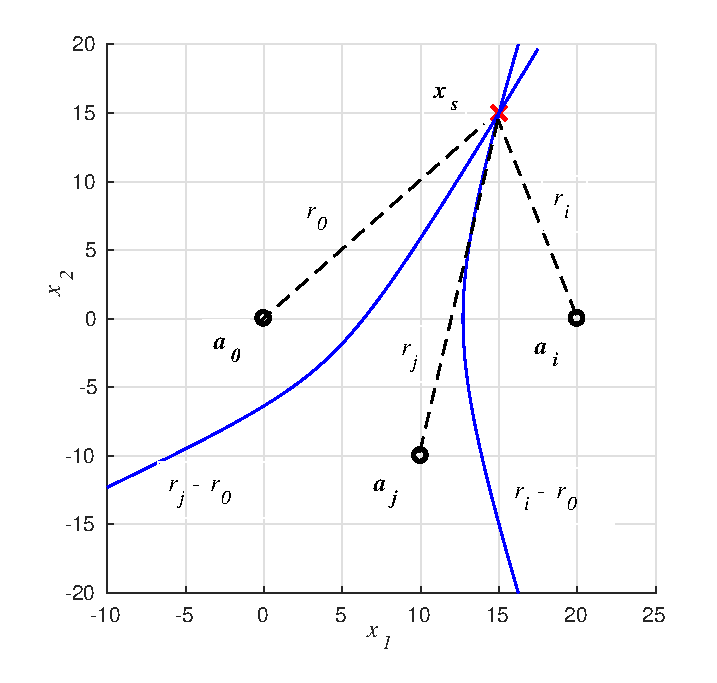
\includegraphics[height=0.45\textheight]{figures/socp_rd/TDOA_example}
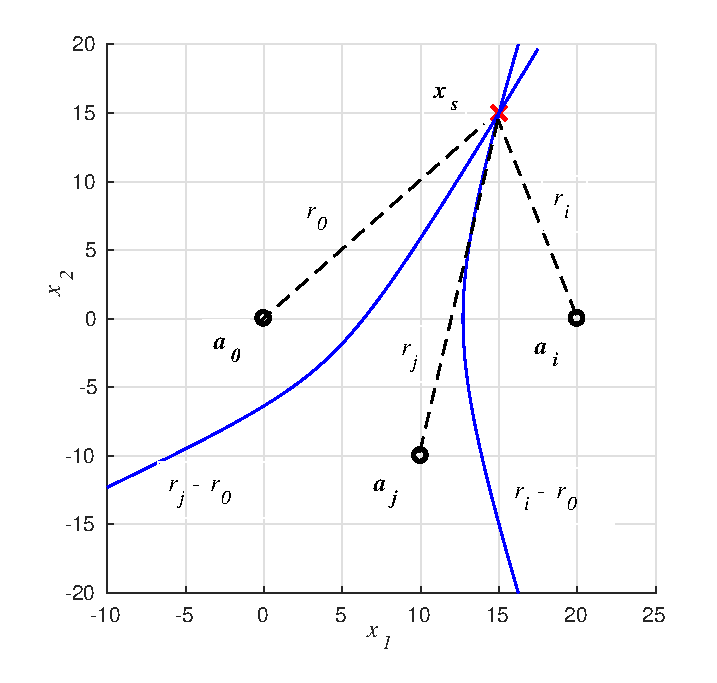
\includegraphics{figures/socp_rd/TDOA_example}
\caption{Range-difference localization.  At least three base stations are required for the planar localization. The red cross indicates the location of the signal source. Sensors are placed at $\protect\Ba_i = (20, 0)^T$, $\protect\Ba_j = (10, -10)^T$, and  $\protect\Ba_0$ is the reference sensor. The time (range) differences $r_j - r_0$ and $r_i - r_0$ form two hyperboloids with focii located at $\protect\Ba_i, \protect\Ba_j$ and $\protect\Ba_0$. Note that the hyperboloids are actually double sheeted, but for visual clarity only the halves which are part of the solution are shown. The intersection of these hyperboloids is the estimated position.
The figure depicts the locus of possible source locations as one half of a two-sheeted hyperboloids.}
\label{fig:tdoa}
\end{figure*}
%
% \phantom{m}
%An example of location estimation using TDOA is shown in Figure \ref{fig:hyperbola}. Consider an instance of the source localization problem on the plane $n = 2$ with the reference sensor $\Ba_0$ placed at the origin and five sensors $m = 5$ located at 
%\begin{equation}
%\nonumber
%\Ba_1 = \begin{bmatrix}
%-5 \\ -13
%\end{bmatrix}, \
%\Ba_2 = \begin{bmatrix}
%-12 \\ 1
%\end{bmatrix},  \
%\Ba_3 = \begin{bmatrix}
%-1 \\ -5
%\end{bmatrix}, \
%\Ba_4 = \begin{bmatrix}
%-9 \\ -12
%\end{bmatrix}, \
%\Ba_5 = \begin{bmatrix}
%-3 \\ -12
%\end{bmatrix}
%\\
%\end{equation}
%
%The source emitting the signal was located at $\Bx_s = (-5,11)^T$. Figure \ref{fig:hyperbola} depicts the locus of possible source locations as one half of a two-sheeted hyperboloids.

%\begin{figure} 
%\centering
%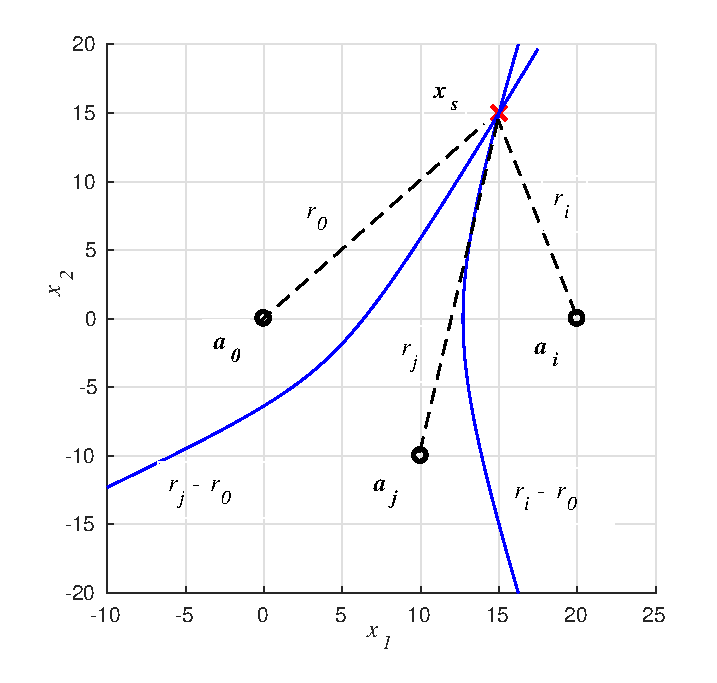
\includegraphics{figures/socp_rd/TDOA_example}
%\caption{Algorithm and contours of the R-LS objective function over the region $\protect\Re = \protect\lbrace \protect\Bx:-15\protect\leq x_1 \protect\leq 15, -25\protect\leq x_2 \protect\leq 15 \protect\rbrace$. The red cross indicates the location of the signal source. Sensors are located at $(-5, -13)^T$, $(-12, 1)^T$, $(-1, -5)^T$, $(-9, -12)^T$ and  $(-3, -12)^T$. Hyperbolas denote possible source locations given the pairwise range-difference readings. Large circles denote possible source locations given the noisy range reading at a particular sensor.}
%\label{fig:hyperbola}
%\end{figure}
 
%Given two base station locations $BS_i$ and $BS_0$, placed at $\Ba_i$ and $\Ba_0$ respectively, with $BS_0$ placed at the origin of the coordinate system, i.e. $\Ba_0 = \symb{0}_n$, and used as a reference station, and a known TDOA, the locus of possible source locations is one half of a two-sheeted hyperboloid. Consider now a third base station $BS_j$ at a third location. This would provide one extra independed TDOA measurement and the source is located on the curve determined by the two intersecting hyperboloids.

%Each TDOA measurement constrains the location of the signal source to be on a hyperboloid with a constant range-difference between the two reference points.

%\textit{Matlab} Using the arrival times, the time differences of arrival between each pair of eNodeBs is calculated using hPositioningTDOA.m. The particular time difference of arrival between a pair of eNodeBs can result from the UE being located at any position where two circles, each centered on an eNodeB, intersect. The two circles have radii which differ by the distance covered at the speed of light in the given time difference. The complete set of possible UE positions across all possible radii for one circle (with the other circle maintaining a radius appropriate to the time difference as already described) forms a hyperbola. The "hyperbolas of constant delay difference" for all the different pairs of eNodeBs are plotted relative to the known eNodeB positions and intersect at the position of the UE.
%A hyperbola is the basis for solving multilateration problems, the task of locating a point from the differences in its distances to given points — or, equivalently, the difference in arrival times of synchronized signals between the point and the given points. Such problems are important in navigation, particularly on water; a ship can locate its position from the difference in arrival times of signals from a LORAN or GPS transmitters. Conversely, a homing beacon or any transmitter can be located by comparing the arrival times of its signals at two separate receiving stations; such techniques may be used to track objects and people. In particular, the set of possible positions of a point that has a distance difference of 2a from two given points is a hyperbola of vertex separation 2a whose foci are the two given points.

%\textit{Wiki} If a pulse is emitted from a platform, it will generally arrive at slightly different times at two spatially separated receiver sites, the TDOA being due to the different distances of each receiver from the platform. In fact, for given locations of the two receivers, a whole set of emitter locations would give the same measurement of TDOA. Given two receiver locations and a known TDOA, the locus of possible emitter locations is one half of a two-sheeted hyperboloid.

%\textit{Wiki} In simple terms, with two receivers at known locations, an emitter can be located onto a hyperboloid.[1] Note that the receivers do not need to know the absolute time at which the pulse was transmitted – only the time difference is needed. A fourth receiver is needed for another independed TDOA, this wil give an extra hyperboloid, the intersection of the curve with this hyperboloid gives one or two solutions, the emitter is then located at the one or at the one of the two solutions.



The localization problem discussed in this section involves a given array of $m+1$ sensors placed in the $n = 2$ or 3 dimensional space with coordinates specified by $\{\Ba_1, \Ba_2, . . . , \Ba_m , a_i \in R^n\}$ and  $\Ba_0 = \symb{0}_n$ placed at the origin and used as a reference sensor. The localization problem here is to estimate the location of a radiating source $\Bx$ given the locations of the $m+1$ sensors and noise-contaminated range-difference measurements $\{d_i, i = 1, 2, \ldots, m\}$ where 
\setcounter{abc}{0}
\begin{equation} \label{eq:6.1}
d_i = \|\Bx - \Ba_i\| - \|\Bx\| + \varepsilon_i, \mbox{ for } i = 1, 2, \ldots, m
\end{equation}
Therefore, the standard range-difference LS (RD-LS) problem is formulated as
\begin{equation} \label{eq:6.2}
\Min \sum^m_{i=1}\left( \|\Bx - \Ba_i\| - \|\Bx\| - d_i\right)^2
\end{equation}
As described in Sec.2.2 of the thesis, finding the solution to ($\ref{eq:6.2}$) is a non-trivial problem and many approaches have been developed to address it. In the following we propose a new iterative procedure to tackle the RD-LS problem (\ref{eq:6.2}), with the goal of achieving a more accurate and robust solution. The central part of the procedure is a convex quadratic programming (QP) problem that needs to be solved in each iteration to provide an increment vector that updates the present iterate to next towards the solution of the localization problem at hand.

\subsection{Sequential Convex Relaxation}

%\newpage 
%
%\input chapters/5/scp_rd_ls
%
%\newpage

We begin by re-writing the unconstrained problem in (\ref{eq:6.2}) as a constrained problem with second-order cone constraints%can be equivalently written as
\setcounter{abc}{0}
\begin{eqnarray} \label{eq:6.3} %1.7
\stepcounter{abc}
\setcounter{equation}{3}
\Min_{\Bx, y, \Bz} & & \sum^m_{i=1}\left( z_i - y - d_i\right)^2\\
\stepcounter{abc}
\setcounter{equation}{3}
\mbox{subject to:}& &\|\Bx - \Ba_i\| = z_i, \quad  i = 1, 2, \ldots m \\
\stepcounter{abc}
\setcounter{equation}{3}
& &\|\Bx\|  = y
\end{eqnarray}
Assume we are in the $k$th iteration and we are to update the $k$th iterate $\{\Bx_k,y_k,\Bz_k\}$. Let the next iterate be
\setcounter{abc}{0}
\begin{eqnarray} \label{eq:6.4} %1.8
\stepcounter{abc}
\Bx^{k+1} &=& \Bx^k + \Bdelta_x \\
\stepcounter{abc}
\setcounter{equation}{4}
y^{k+1} &=& y^k + \delta_y \\
\stepcounter{abc}
\setcounter{equation}{4}
\Bz^{k+1} &=& \Bz^k + \Bdelta_z
\end{eqnarray}
where $\{\Bdelta_x, \delta_y, \Bdelta_z\}$
are such that the objective function in (
\ref{eq:6.4}a) is reduced and, at the same time, the constraints in (\ref{eq:6.3}b) and (\ref{eq:6.3}c) are better approximated at $\{\Bx_{k+1},y_{k+1},\Bz_{k+1}\}$ in the sense that
\setcounter{abc}{0}
\begin{eqnarray}
\nonumber
\|\Bx_{k+1} - \Ba_i\| &\approx &z_i^{k+1}, \quad i = 1, 2, \ldots, m \\
\nonumber
\|\Bx_{k+1}\| &\approx &y_{k+1}
\end{eqnarray}
namely,
\setcounter{abc}{0}
\begin{eqnarray}
\nonumber
\|\Bx_{k} + \Bdelta_x - \Ba_i\| &\approx &z_i^{k} + \Bdelta_{z_i}, \quad i = 1, 2, \ldots, m \\
\nonumber
\|\Bx_{k} + \Bdelta_x\| &\approx &y_{k}  + \Bdelta_y
\end{eqnarray}
By replacing the left-hand sides of the above equations with their first-order Taylor approximations, we obtain
\setcounter{abc}{0}
\begin{eqnarray}
\nonumber
\|\Bx_{k} - \Ba_i\| + \partial_x^T\|\Bx_{k} - \Ba_i\|\Bdelta_x &\approx & z_i^{k} + \Bdelta_{z_i}, \quad i = 1, 2, \ldots, m \\
\nonumber
\|\Bx_{k}\|  + \partial_x^T\|\Bx_{k}\|\Bdelta_x\ &\approx & y_{k}  + \Bdelta_y
\end{eqnarray}
where $\partial_x$ is the subdifferential operator with respect to variable $\Bx$. Assuming $\Bx_k \neq \Ba_i$ and $\Bx_k$ is nonzero, then
\begin{equation}
\nonumber
\partial_x\|\Bx_{k} - \Ba_i\| = \frac{\Bx_{k} - \Ba_i}{\|\Bx_{k} - \Ba_i\|} \ \mbox{and } \partial_x\|\Bx_{k}\| = \frac{\Bx_{k}}{\|\Bx_{k}\|}
\end{equation}
Hence
\setcounter{abc}{0}
\begin{eqnarray} \label{eq:6.5} %1.9
\stepcounter{abc}
\|\Bx_k - \Ba_i\| + \frac{\left(\Bx_{k} - \Ba_i\right)^T\Bdelta_x}{\|\Bx_k - \Ba_i\|} &\approx &z^{(k)}_i + \delta_{z_{j}}, \quad i = 1, 2,...,m \\
\stepcounter{abc}
\setcounter{equation}{5}
\|\Bx_k\| + \frac{\Bx_{k}^T\Bdelta_x}{\|\Bx_k\|} &\approx &y_k + \delta_y
\end{eqnarray}
The objective in (\ref{eq:6.3}a) can be written as
 \setcounter{abc}{0}
\begin{eqnarray} 
\nonumber
F(\Bx_{k+1}) & =  & \sum^m_{i = 1} \left(z^{(k)}_i + \delta_{z_i} - (y_k + \delta_y) - d_i \right)^2 \\
\nonumber
& = & \sum^m_{i = 1} \left(- \delta_y + \delta_{z_i}  - \tilde{d_i^{(k)}} \right)^2
\end{eqnarray}
where 
\begin{equation}
\nonumber
\tilde{d}^{(k)}_i =  d_i - y_k - z_i^{(k)}
\end{equation}
are grouped known constant terms. Based on the above, the problem to be solved in the \textit{k}th iteration is formulated as
\setcounter{abc}{0}
\begin{eqnarray} \label{eq:6.6} %1.10
\stepcounter{abc}
\Min_{\tilde{\Bdelta}}& &f(\tilde{\Bdelta}) = \sum^m_{i=1}\left(-\delta_y + \delta_{z_{j}} - \tilde{d^{(k)}_i}\right)^2\\
\stepcounter{abc}
\setcounter{equation}{6}
\mbox{subject to:}& &\|\Bx_k - \Ba_i\| + \frac{\left(\Bx_{k} - \Ba_i\right)^T\Bdelta_x}{\|\Bx_k - \Ba_i\| } = z_i^{(k)} + \delta_{z_{j}}, \\
\nonumber
& &\qquad \qquad \qquad \qquad \qquad \qquad \qquad  \qquad i = 1, 2, \ldots m \\
\stepcounter{abc}
\setcounter{equation}{6}
& &\|\Bx_k\| + \frac{\Bx_k^T\Bdelta_x}{\|\Bx_k\|} = y_k + \delta_y \\
\stepcounter{abc}
\setcounter{equation}{6}
& &\begin{bmatrix}
-\beta\BOne_2 \\
-\beta \\
-\beta\BOne_m
\end{bmatrix} \leq \begin{bmatrix}
\Bdelta_x \\
\delta_y \\
\Bdelta_z
\end{bmatrix} \leq \begin{bmatrix}
\beta\BOne_2 \\
\beta \\
\beta\BOne_m
\end{bmatrix}
\end{eqnarray}
The constraints in (\ref{eq:6.6}d) assure that the magnitude of each component in $\{\Bdelta_x, \delta_y, \Bdelta_z\}$ is no greater than $\beta$. %, but also they assure that all components of $\{y_{k + 1}, \Bz_{k + 1}\}$ are nonnegative as long as $\{y_{k}, \Bz_{k}\}$ are nonnegative, which are natural to impose as can be seen from (\ref{eq:6.3}b) and (\ref{eq:6.3}c) because they are vector norms. 
Obviously, the problem in (\ref{eq:6.6}) is a convex QP problem. One technical difficulty that may occur in solving problem (\ref{eq:6.6}) is that the feasible region defined by (\ref{eq:6.6}b), (\ref{eq:6.6}c), and (\ref{eq:6.6}d) may be empty. In such a case the constraints in problem (\ref{eq:6.6})
must be adequately relaxed in order for the problem to be solvable. To this end we express the problem in (\ref{eq:6.6}) in a more compact form as
\setcounter{abc}{0}
\begin{eqnarray} \label{eq:6.7} %1.11
\stepcounter{abc}
\Min_{\Bdelta}& &f\left(\tilde{\Bdelta}\right) \\
\stepcounter{abc}
\setcounter{equation}{7}
\mbox{subject to}& &\BA_k\tilde{\Bdelta} = \Bb_k \\
\stepcounter{abc}
\setcounter{equation}{7}
& &\BC\tilde{\Bdelta} \leq \Bq
\end{eqnarray}
where the objective function is
\setcounter{abc}{0}
\begin{eqnarray}
\nonumber
f\left(\tilde{\Bdelta}\right) = \|\BS\tilde{\Bdelta} - \tilde{\Bd_k} \|_2
 %\| -\delta_y\symb{1_m} + \Bdelta_z - \tilde{\Bd_k} \|_2
\end{eqnarray}
and
\setcounter{abc}{0}
\begin{equation}\label{eq:6.8}
\stepcounter{abc}
\BS = \begin{bmatrix}
\symb{0}_{m \times 1} & -\symb{1}_{m \times 1} & -\symb{I}_m
\end{bmatrix} , 
\tilde{\Bdelta} = \begin{bmatrix}
\Bdelta_x \\
\delta_y \\
\Bdelta_z
\end{bmatrix} , 
\BA_k = \begin{bmatrix}
\BA_1^{(k)} & \symb{0}_{m \times 1} & -\symb{I}_m \\
\Bx_k & -1 & \symb{0}_{1 \times m}\\
\end{bmatrix} 
\end{equation}
\setcounter{abc}{1}
\begin{equation}
\stepcounter{abc}
\setcounter{equation}{8}
\BA_1^{(k)} = \begin{bmatrix}
\frac{\left(\Bx_k - \Ba_1\right)^T}{\|\Bx_k - \Ba_1\|} \\
\frac{\left(\Bx_k - \Ba_2\right)^T}{\|\Bx_k - \Ba_2\|} \\
\vdots \\
\frac{\left(\Bx_k - \Ba_m\right)^T}{\|\Bx_k - \Ba_m\|} \\
\end{bmatrix}, 
\quad \Bb_k = \begin{bmatrix}
z_1^{(k)} - \|\Bx_k - \Ba_1\| \\
z_2^{(k)} - \|\Bx_k - \Ba_2\| \\
\vdots \\
z_m^{(k)} - \|\Bx_k - \Ba_m\| \\
y_k - \|\Bx_k\| \\
\end{bmatrix}
\end{equation}
\begin{equation}
\stepcounter{abc}
\setcounter{equation}{8}
\tilde{\Bd_k} = 
\begin{bmatrix}
d_1 + y^k - z_1^k \\
d_2 + y^k - z_2^k \\
\vdots \\
d_m + y^k - z_m^k \\
\end{bmatrix},
\BC = \begin{bmatrix}
\symb{I}_{m+3} \\
-\symb{I}_{m+3}
\end{bmatrix},
\Bq = \beta\Be
\end{equation}
\noindent
where $\Be = \symb{1}_{2(m+3)}$ is the all-one vector of dimension $2(m+3)$. By introducing nonnegative slack variables $\Bu, \Bv$, and $w$, we relax the problem in (\ref{eq:6.7}) to
\setcounter{abc}{0}
\begin{eqnarray} \label{eq:6.9} %1.12
\stepcounter{abc}
\Min_{\Bdelta}& &f\left(\tilde{\Bdelta}\right) + \tau\sum_{i=1}^{m+1} \left(u_i + v_i\right) +\tau w\\
\stepcounter{abc}
\setcounter{equation}{9}
\mbox{subject to}& &\BA_k\tilde{\Bdelta} - \Bb_k = \Bu - \Bv \\
\stepcounter{abc}
\setcounter{equation}{9}
& &\BC\tilde{\Bdelta} - \Bq \leq w\Be \\
\stepcounter{abc}
\setcounter{equation}{9}
& & \Bu \geq \symb{0}, \Bv \geq \symb{0}, w \geq 0
\end{eqnarray}
where $\tau > 0$ is a sufficiently large scalar. It is easy to verify that the feasible region defined by (\ref{eq:6.9}b) -  (\ref{eq:6.9}d) is always nonempty. For example, if we fix $\tilde{\Bdelta} = \tilde{\Bdelta_0}$ arbitrarily, then obviously the point $\{\tilde{\Bdelta_0}, \Bu_0, \Bv_0, w_0\}$ with
\setcounter{abc}{0}
\begin{equation}
\nonumber
\Bu_0 = \mbox{max}\{\symb{0},\BA_0\tilde{\Bdelta_0} -\Bb_0\}, \quad \Bv_0 = \mbox{max}\{\symb{0},-(\BA_0\tilde{\Bdelta_0} -\Bb_0)\}, \mbox{and } w_0 = \mbox{max}\{0,\BC\tilde{\Bdelta_0} -\Bq\}
\end{equation}

\noindent
is a feasible point for problem (\ref{eq:6.9}). Penalty terms $\tau\sum_{i=1}^{m+1} \left(u_i + v_i\right) +\tau w$ are included in the objective function in (\ref{eq:6.9}a) in order to reduce the magnitudes of the slack variables while minimizing the original objective function. If the solution slack variables turn out to be all zero, then the solution  of (\ref{eq:6.9}) also solves problem (\ref{eq:6.7}). Otherwise, we conclude that problem (\ref{eq:6.7}) in not solvable and the solution obtained by solving (\ref{eq:6.9}) is a reasonable candidate for the $k$th iteration to update $\{\Bx_k, y_k, \Bz_k\}$.

\subsection{The Algorithm}

The input parameters for the algorithm include the bound $\beta$ on the increment vector $\tilde{\Bdelta} =\left(
\Bdelta_x, \delta_y, \Bdelta_z\right)$. It controls the size of a "trust region" over which a convex subproblem is carried out and is responsible for the performance of the algorithm. If parameter $\beta$ is chosen too large, then approximation $\Bx_{k+1}$ will perform poorly because in this case the convex model is less accurate \cite{OPTII}. If $\beta$ is too small the progress of the algorithm will be too slow. In our simulations a $\beta$ between 3 and 6 was found to work very well. Other input parameters are initial point $\Bx_0$, initial weight for penalty terms $\tau_0$, and upper limit of the weight  $\tau_{max}$ (to avoid numerical problems that may occur  if $\tau_k$ becomes too large).

We remark that the method proposed in this section is \textit{local}, therefore is not guaranteed to converge to the global minimum when applied to the nonconvex problem. As discussed in Sec. 2.2 of the thesis, the original LS objective in (\ref{eq:6.2}) is highly nonconvex with many local minimums even for small-scale systems. Consequently, the choise of a good initial point is critical to ensure good performance of the method. Several techniques are available, these include: i) set the initial point to the origin; ii) select the initial point uniformly randomly over the same region as the unknown radiating source; iii) run the algorithm from a set of candidate initial points and identify the solution as the one with lowest LS error.  The candidate initial points can be selected either randomly over the region or based on some  a priori information, for example, the geometry of the sensor network; iv) solve an approximating problem or apply a “global” localization algorithm such as those in \cite{BeckStLi} to generate an approximate LS solution, then take it as the initial point to run the proposed algorithm. 

Based on the analysis above, the localization algorithm for range-difference measurements can be outlined as follows. For the ease of notation we will refer to the proposed algorithm as Sequential Convex Relaxation for Range-Difference-based Least Squares (SCR-RDLS).

%The constraint $\beta$ was imposed on each element of the vector $\tilde{\Bdelta}$ to guarantee that at each iteration is sufficiently small.

%Dropping the constraints in \ref{eq:6.8}f,g allows more variety in choosing the search direction, which increases the likelihood of the algorithm not to get trapped in the local minimimum.

\phantom{m}
\framebox{%
\parbox{5.4in}{
\label{alg:scp_rd}
\phantom{m}

\noindent \textbf{Algorithm 4. Sequential Convex Relaxation for Range-Difference Localization}

\phantom{m}

1) Input data: Sensor locations $\{\Ba_i, i=1,\ldots,m\}$, range-difference measurements $\{d_i, i=1,\ldots,m\}$, initial point $\Bx_0$, initial weight $\tau_0$ and upper limit of weight $\tau_{max}$, increment bound $\beta$ and convergence tolerance $\epsilon$. %\gamma, \sigma$, 
Set iteration count to $k = 0$. Form $\BS, \BC$ and $\Bq$ as
\setcounter{abc}{0}
\begin{equation}
\nonumber
\BS = \begin{bmatrix}
\symb{0}_{m \times 1} & -\symb{1}_{m \times 1} & -\symb{I}_m
\end{bmatrix},
\BC = \begin{bmatrix}
\symb{I}_{m+3} \\
-\symb{I}_{m+3}
\end{bmatrix},
\Bq = \beta\Be
\end{equation}
%\phantom{m}

2) Form $y_k$ and $\Bz_k$ as
\begin{equation}
\nonumber
y_k =\|\Bx_k\|, \Bz_k = \begin{bmatrix}
\|\Bx_k - \Ba_1\| \\
\vdots \\
\|\Bx_k - \Ba_m\|
\end{bmatrix} 
\end{equation}
form $\BA_k, \tilde{\Bd_k}, \Bb_k$ and $\BC_k $ as in (\ref{eq:6.8}) and solve
%\phantom{m}
%\noindent
\setcounter{abc}{0}
\begin{eqnarray} 
\nonumber
\Min_{\Bdelta}& &f\left(\tilde{\Bdelta}\right) + \tau_k\sum_{i=1}^{m+1} \left(u_i + v_i\right) +\tau_k w\\
\nonumber
\mbox{subject to}& &\BA_k\tilde{\Bdelta} - \Bb_k = \Bu - \Bv \\
\nonumber
& &\BC\tilde{\Bdelta} - \Bq \leq w\Be \\
\nonumber
& & \Bu \geq \symb{0}, \Bv \geq \symb{0}, w \geq 0
\end{eqnarray}
\noindent
Denote the solution as $\tilde{\Bdelta}_k = (\Bdelta_x^*, \delta_y^*, \Bdelta_z^*)$. 

%\phantom{m}

3) Update  $\tau_{k+1} $ = min $(1.5\tau_k, \tau_{max})$, set $k = k+1$. Update $\tilde{\Bx}^{*}$ to
\setcounter{abc}{0}
\begin{eqnarray} 
\nonumber
\Bx^{*} = \Bx^k + \Bdelta_x^* \\
\nonumber
y^{*} = y^k + \delta_y^* \\
\nonumber
\Bz^{*} = \Bz^k + \Bdelta_z^*
\end{eqnarray}

%\phantom{m}

4) If $\|\tilde{\Bdelta}_k\| \leq \epsilon$, terminate and output $\Bx^*$ as the solution; otherwise, set $\tilde{\Bx}_{k} = \Bx^{*}$  and repeat from Step 2. 

\phantom{m}
}
}

\subsection{Numerical Results}

Performance of the proposed algorithm was evaluated and compared with existing state-of-the-art methods by Monte Carlo simulations with a set-up similar to that of \cite{BeckStLi}. SRD-LS solutions were used as performance benchmarks for the Algorithm 4. The sensor network consisted of $11$ sensors with $\Ba_0 = \BO$ placed at the origin and other ten sensors  $\{\Ba_i, i = 1, 2,\ldots,10\}$ randomly placed in the planar region in $[-15;15]\times[-15;15]$. A radiating source $\Bx_s$ was located randomly in the region $\{\Bx=[x_1;x_2], -10\leq x_1,x_2\leq 10\}$. The coordinates of the source and sensors were generated for each dimension following a uniform distribution. Measurement noise $\{\varepsilon_i, i=1,\ldots,m\}$ was modelled as independent and identically distributed (i.i.d) random variables with zero mean and variance $\sigma^2$, with $\sigma$ being one of four possible levels $\{10^{-3}, 10^{-2}, 10^{-1}, 1\}$.  The range-difference measurements $\{d_i, i=1, 2,\ldots,10\}$ were calculated using (\ref{eq:6.1}). Accuracy of source location estimation was evaluated in terms of average of the squared position error in the form $\|\Bx^*-\Bx_s\|^2$, where $\Bx_s$ denotes the exact source location and $\Bx^*$ is its estimation obtained by SRD-LS and proposed methods, respectively.  
In our simulations parameter $\beta$ was set to 3, the initial penalty term $\tau_0$, and upper limit of the penalty term $\tau_{max}$ were set to 10 and 10 000 respectively. The proposed method was implemented by using  CVX  \cite{cvx} and implementation of SRD-LS followed \cite{BeckStLi}. In our simulations we set the initial point $\Bx_0$ to the solution of the following subproblem
\setcounter{abc}{0}
\begin{eqnarray} \label{eq:initpnt}
\nonumber
\Min_{\Bx, y, \Bz} & &\sum^m_{i=1}\left( z_i - y - d_i\right)^2\\
\nonumber
\mbox{subject to:}& &\|\Bx - \Ba_i\| \leq z_i, \quad  i = 1, 2, \ldots m \\
\nonumber
& &\|\Bx\|  \leq y
\end{eqnarray}
\noindent
The iterations proceeded until the magnitude of the increment vector $\|\tilde{\Bdelta}_k\|$ falls below a convergence tolerance $\epsilon$ which was set to $\epsilon = 10^{-6}$. 

Table \ref{tab:scr_rdls}  provides comparisons of the SCR-RDLS with SRD-LS, where each entry is averaged squared error over 1,000 Monte Carlo runs of the method. %The MLE was implemented using Matlab function \textit{lsqnonlin} \cite{matlab}, initialized with the same point as PCCP.
 It is observed that, comparing with SRD-LS, the estimates produced by the proposed algorithm are found to be closer to the true source locations in MSE sense. The last column of the table  represents relative improvement (R.I.) of the proposed method over SRD-LS solutions in percentage. Further analysis of the data that was used to generate Table \ref{tab:scr_rdls} illustrates the advantage of the SCR-RDLS solution over the SRD-LS. 
Each entry in Table \ref{tab:rdls} is a standard deviation of the squared  estimation errors  aggregated over the  same 1,000 Monte Carlo runs described above in Table \ref{tab:scr_rdls} where the MSEs of the position estimation are shown. The results summarized in Table \ref{tab:rdls} indicate that the SCR-RDLS algorithm provides considerable performance improvement relative to the SRD-LS algorithm.

\phantom{m}

\begin{table}[h]
\centering
\caption{MSE of position estimation for SRD-LS and SCR-RDLS methods}
\phantom{m}
\begin{tabular}{|c|c|c|c|} \hline
\centering
$\sigma$ & SRD - LS & SCR-RDLS & (R.I.,\%)  \\ \hline
%&&& \\
1e-03&	1.2655e-06  & 8.4626e-07 &  33 \\ &&&\\
1e-02&	1.4492e-04 &  6.8385e-05 &  52 \\ &&&\\
1e-01&	1.3329e-02 & 7.1676e-03 &   46 \\ &&&\\
1e+0&	1.6077e+00 &  9.5371e-01 &   40  \\ %&&&\\
\hline
\end{tabular}
\label{tab:scr_rdls}
%\end{table}
%\begin{table}[h]

\phantom{m}

\centering
\caption{Standard deviation of the squared position estimation error for SRD-LS and SCR-RDLS methods}
\phantom{m}
\begin{tabular}{|c|c|c|} \hline
$\sigma$ & SRD - LS & SCR-RDLS  \\ \hline
%&&& \\ 
1e-03&	3.3990e-06 &  3.2917e-06 \\ &&\\
1e-02&	5.9818e-04 &   1.3673e-04 \\ &&\\
1e-01&	3.6154e-02  & 2.4337e-02 \\ &&\\
1e+0&	4.2206e+00 &  3.4931e+00 \\ %&&&&\\
\hline
\end{tabular}
\label{tab:rdls}
\end{table}

\phantom{m}

%\newpage
\input chapters/5/range_based


\section{Execution Time Comparison}

In this section we compare the average running time of the proposed algorithms for range and range-difference measurements. The algorithms have been implemented in Matlab using CVX [16] (Processor 1.8 GHz Intel Core i3, Memory 4 GB 1600 MHz DDR3). Each of the algorithms has been implemented using the initialization set-up described in the Numerical Results section of the relevant chapter. The noise level was set to $\sigma = 0.2$.

We run each algorithm 1000 times and compute the average execution time in milliseconds (Tables 4.5 and 4.7). Then we compare the running time with respect to the IRWSR-LS (Table 4.6) and IRWSRD-LS (Table 4.8). The complexity of IRWSR-LS (IRWSRD-LS) is that of the SR-LS (SRD-LS) times the number of re-weighting iterations. This approach is the fastest of all those proposed since at each iteration the solution is found in a closed form.  For the PCCP and SCR-RLS methods  each iteration involves solving an SOCP problem, and a convex QP problem in the case of SCR-RDLS.

\begin{table}[h]
\label{tab:absR}
\centering
\caption{Performance Comparison of Range-Based Algorithms. Absolute CPU time usage}
\phantom{m}
\begin{tabular}{|c|c|} 
\hline
Method &  Absolute time, ms.\\ \hline
%SR-LS & 1.1789e+00 \\&\\
IRWSR-LS  & 6.0777e+00 \\&\\
PCCP & 5.3790e+03 \\&\\
SCR-RLS & 3.7005e+03  \\ %&&&\\
\hline
\end{tabular}
%\begin{tabular}{||c||c|c|c||} 
%\hhline{|t:====:t|} 
%$\sigma$ & IRWSR-LS  & PCCP & SCR-RLS  \\ \hline
%%&&& \\
%1e-03&	  &   &   \\ &&&\\
%1e-02&	  &   &   \\ &&&\\
%1e-01&	  &   &    \\ &&&\\
%1e+0&	  &   &     \\ %&&&\\
%\hhline{|b:====:b|} 
%\end{tabular}
\end{table}


\begin{table}[h]
\label{tab:relR}
\centering
\caption{Performance Comparison of Range-Based Algorithms. Relative CPU time usage}
\phantom{m}
\begin{tabular}{|c|c|} 
\hline
Method &  Relative time\\ \hline
%SR-LS & 1 \\&\\
IRWSR-LS  & 1 \\&\\
PCCP & 885 \\&\\
SCR-RLS &  609  \\ %&&&\\
\hline
\end{tabular}
\end{table}



\begin{table}[h]
\label{tab:absRD}
\centering
\caption{Performance Comparison of Range-Difference-Based Algorithms. Absolute CPU time usage}
\phantom{m}
\begin{tabular}{|c|c|} 
\hline
Method &  Absolute time, ms.\\ \hline
%SRD-LS & 1.7581e+00 \\&\\
IRWSRD-LS  & 7.4039e+00 \\&\\
SCR-RDLS &  3.6347e+03  \\ %&&&\\
\hline
\end{tabular}
\end{table}



\begin{table}[h]
\label{relRD}
\centering
\caption{Performance Comparison of Range-Difference-Based Algorithms. CPU time usage}
\phantom{m}
\begin{tabular}{|c|c|} 
\hline
Method &  Relative time\\ \hline
%SRD-LS & 1 \\&\\
 IRWSRD-LS  & 1 \\&\\
SCR-RDLS &  490  \\ %&&&\\
\hline
\end{tabular}
\end{table}

%	\startchapter{Conclusion}

\section{Conclusion}


\section{Future Work}

Influense of sensor geometry on the accuracy of the proposed methods. For example, one of the highest impacts on accuracy degradation is Geometric Dilusion of Presicion. Optimum sensor arrangement is a separate research area. 

Multi-source localization, when the range measurements were obtained from the energy-based readings. 
	\appendix
	\startappendix{}
\label{chapter:app1}

\section{Solving \ref{eq:3.16}}

% TODO reword as this is too similar to contents of paper 'original.pdf'
Next we show how to compute an exact solution to the SR-LS problem
(\ref{eq:3.16}). Note that \ref{eq:3.16} belongs to the class of problems
consisting of minimizing a quadratic function subject to a single
quadratic constraint. Problems of this type are called generalized trust
region subproblems (GTRS) \cite{More}. GTRS problems, although usually 
nonconvex, possess necessary and sufficient optimality conditions from
which efficient solution methods can be derived. In particular, by 
Theorem 3.2 of \cite{More}, $\By \in R^{n+1}$ is an optimal solution
of \ref{eq:3.16} if and only if there exists $\lambda \in R^{n}$ 
such that

\begin{equation} \label{eq:A.1}
(\BA^{T}\BA + \lambda\BD)\By = \BA^{T}\Bb - \lambda\Bf
\end{equation}

\begin{equation} \label{eq:A.2}
\By^{T}\BD\By + 2\Bf^{T}\By = 0
\end{equation}

\begin{equation} \label{eq:A.3}
\BA^{T}\BA + \lambda\BD \geq 0
\end{equation}

It follows that the optimal solution of \ref{eq:3.16} is given by

\begin{equation} \label{eq:A.4}
\hat{\mathbf{y}}(\lambda) = (\BA^{T}\BA + \lambda\BD)^{-1}(\BA^{T}\Bb - \lambda\Bf)
\end{equation}

where $\lambda$ is the unique solution of

\begin{equation} 
\label{eq:A.5}
\varphi(\lambda) = 0, \lambda \in I
\end{equation}

and the function $\varphi$ is defined by

\begin{equation} \label{eq:A.6}
\varphi(\lambda) \equiv \hat{\mathbf{y}}(\lambda)^{T}\BD\hat{\mathbf{y}}(\lambda) + 2\Bf^{T}\hat{\mathbf{y}}(\lambda)
\end{equation}

The interval $I$ consists of all $\lambda$ for which 
$\BA^{T}\BA + \lambda\BD$ is positive definite, which immediately implies
that 

\begin{equation} \label{eq:A.7}
I = \left(-\dfrac{1}{\lambda_1(\BD,\BA^{T}\BA)}, \infty\right)
\end{equation}

Moreover, it is known by Theorem 5.2 of \cite{More} that
$\varphi(\lambda)$ is strictly decreasing over $I$ and therefore
a simple bisection algorithm can be used to find the optimal $\lambda$
over the interval $I$.

Note that we have limited the discussion to the case in which 
$\BA^{T}\BA + \lambda\BD$ is strictly positive definite, which is
equivalent to saying that the optimal $\lambda$ is different from
$-1/\lambda_1(\BD, \BA^{T}\BA)$. The case in which the optimal $\lambda$
is equal to $-1/\lambda_1(\BD, \BA^{T}\BA)$ is the so-called
``hard case'' of the GRTS problem \cite{FortinWol}, which can 
also be treated by a more refined analysis. However, the value 
$\lambda = -1/\lambda_1(\BD, \BA^{T}\BA)$ 
is very unlikely to occur both theoretically and practically
(it never occurred in the tens of thousands of simulations we 
have performed). Therefore, for the sake of simplicity, we have
tacitly assumed that $\BA^{T}\BA + \lambda\BD$
is positive semi-definite.

The procedure for calculating the SR-LS estimate is summarized next:

a) Use a bisection algorithm to obtain a solution $\lambda$ to (\ref{eq:A.5}).

b) The SR-LS estimate is given by the first $n$ components of the 
vector $\hat{\mathbf{y}}(\lambda)$ in \ref{eq:A.4}.

An alternative approach for computing the SR-LS estimate is considered
in \cite{CheungChan}. The method in \cite{CheungChan} consists of 
finding all the five roots
of the equation $\varphi(\lambda) = 0$ over the real line. This is done
by invoking a root finding procedure for polynomials of degree five.
In a second stage, the global optimal solution of SR-LS is chosen as
the best of the derived possible solutions. Interestingly, in the
above we proved that there is no need to find all the roots of
$\varphi(\lambda) = 0$ and that a simple bisection algorithm is 
sufficient.

\section{Simultaneous Matrix Diagonalization}

\begin{equation} \label{eq:A.5}
\Bv^{T}(\BB^{T}\BB)\Bv = \|\BB\Bv\|^{2} 
\end{equation}

$\BB^{T}\BB$ is at least PSD (full rank), ?? x ??

\begin{equation} \label{eq:A.6}
\BU^{T}\BB^{T}\BB\BU = \begin{bmatrix}
\lambda_1 & & 0 \\
 & \ddots & \\
0 & & \lambda_n
\end{bmatrix}
\end{equation}

$\BU^{T}\BC\BU$ is symmetric.

Non-symmetric square root (of $\BB^{T}\BB$):

\begin{equation} \label{eq:A.7}
\BU\begin{bmatrix}
\sqrt{\lambda_1} & & 0 \\
 & \ddots & \\
0 & & \sqrt{\lambda_n}
\end{bmatrix}
\end{equation}

Symmetric square root:

\begin{equation} \label{eq:A.8}
\BB^{T}\BB = \BU\begin{bmatrix}
\lambda_1 & & 0 \\
 & \ddots & \\
0 & & \lambda_n
\end{bmatrix}\BU^{T} = \BU\begin{bmatrix}
\sqrt{\lambda_1} & & 0 \\
 & \ddots & \\
0 & & \sqrt{\lambda_n}
\end{bmatrix}\BU^{T}\BU\begin{bmatrix}
\sqrt{\lambda_1} & & 0 \\
 & \ddots & \\
0 & & \sqrt{\lambda_n}
\end{bmatrix}\BU^{T}
\end{equation}

i.e.

\begin{equation} \label{eq:A.9}
\BB^{T}\BB = (\BB^{T}\BB)^{1/2}(\BB^{T}\BB)^{1/2}
\end{equation}

\begin{equation} \label{eq:A.10}
\BV(\BB^{T}\BB)^{-1/2}(\BB^{T}\BB)(\BB^{T}\BB)^{-1/2}\BV^{T} = \BV\BI\BV = \begin{bmatrix}
\gamma_1 & & 0 \\
 & \ddots & \\
0 & & \gamma_{n+1}
\end{bmatrix}
\end{equation}

Then for the matrix $\BC$:

\begin{equation} \label{eq:A.11}
\BV(\BB^{T}\BB)^{-1/2}\BC(\BB^{T}\BB)^{-1/2}\BV^{T} = \begin{bmatrix}
\delta_1 & & 0 \\
 & \ddots & \\
0 & & \delta_{n+1}
\end{bmatrix}
\end{equation}

where $\BV$ is orthogonal.

Hence the matrix $\BP$ we seek to compute is given by:

\begin{equation} \label{eq:A.12}
\BP = (\BB^T\BB)^{-1/2}\BV^T
\end{equation}

Share same eigenspace, i.e. the basis of the eigenspace is the same.

\begin{eqnarray}
\BP^{-1}\BA\BP = diag\{\lambda_A\} \\
\nonumber
\BP^{-1}\BB\BP = diag\{\lambda_B\}
\end{eqnarray}

Eigenspace $\BE_{\lambda A}$ of $\BA$ is equivalent to null 
space of $(\BA - \lambda_A\BI)$. 
Hence for $(\BB^T\BB)$ rank = 2 it is true
that

\begin{eqnarray}
\BA = \BV\BLambda_a\BV^T \\
\BB = \BV\BLambda_b\BV^T \\
\BB\BA = \BV\BLambda_b\BV^T\BV\BLambda_a\BV^T = \BV\BLambda_b\BLambda_a\BV^T \\
\Leftrightarrow \BA\BB = \BV\BLambda_a\BLambda_b\BV^T
\end{eqnarray}

for the case when $\BA\BB = \BB\BA$.

\begin{eqnarray}
\nonumber
\BA\BV = \BB\BV\BD \\
\nonumber
\BA = \BP\BLambda_a\BP^T \\
\nonumber
\BB = \BP\BLambda_b\BP^T \\
\nonumber
\BH\BP = \BP\BLambda_a \\
\nonumber
\BB\BP = \BP\BLambda_b \Rightarrow \BP = \BB^{-1}\BP\BLambda_b \\
\nonumber
\BA = \BB\BV\BD\BV^T \\
\nonumber
\BP\BLambda_a\BP^T = \BP\BLambda_b\BP^T\BV\BD\BV^T \\
\nonumber
\BA\BB^{-1}\BP\BLambda_b = \BB^{-1}\BP\BLambda_b\BLambda_a \\
\nonumber
\BB\BA\BB^{-1}\BP = \BP\BLambda_b\BLambda_a\BLambda_b^{-1} \\
\nonumber
\BA = \BP\BLambda_a\BP^T
\end{eqnarray}

Decomposition of $\BB^T\BB$:

\begin{eqnarray}
\nonumber
[\BV, \BD] = eig(\BB^T\BB) \\
\nonumber
\Bd = diag(\BD) \\
\nonumber
\Bd_1 = -1/\sqrt{\Bd} \\
\nonumber
\BD_1 = diag(\Bd_1) \\
\nonumber
\BS_{b+b} = \BV\BD_1\BV^T = (\BB^T\BB)^{-1/2} \\
\nonumber
[\BV, \Bh] = eig(\BS_{b+b}\BC\BS_{b+b}) \\
\nonumber
\BP = \BS_{b+b}\BV^T
\end{eqnarray}

To ensure that all computations were performed correctly,
the following should hold:

\begin{equation}
\BP^T\BB^T\BB\BP \equiv \BI
\end{equation}

\section{Solving \ref{eq:3.32}}

\subsection{Finding roots of the polynomial}

\begin{eqnarray}
\sum^{n+1}_{j=1} \frac{f^2_j\delta_j}{\left(\gamma_j+\lambda\delta_j\right)^2} = 0 \\
\nonumber
\Leftrightarrow \sum^{n+1}_{j=1} f^2_j\delta_j \prod^{n+1}_{k=1,k\neq j}\left(\gamma_k + \lambda_k\delta_k\right)^2 = 0 
\end{eqnarray}
For the planar case, i.e. n = 2
\begin{equation}
\nonumber
\begin{aligned}
& f^2_1\delta_1(1 + \lambda\delta_2)^2(1 + \lambda\delta_3)^2 + f^2_2\delta_2(1 + \lambda\delta_1)^2(1 + \lambda\delta_3)^2 + f^2_3\delta_3(1 + \lambda\delta_2)^2(1 + \lambda\delta_1)^2 \\ 
& = a_0 + \lambda a_1 + \lambda^2 a_2 + \lambda^3 a_3 + \lambda^4 a_4
\end{aligned}
\end{equation}

\begin{eqnarray}
\nonumber
a_0 = f^2_1\delta_1 + f^2_2\delta_2 + f^2_3\delta_3 \\
\nonumber
a_1 = f^2_1\delta_1(2\delta_2 + 2\delta_3) + f^2_2\delta_2(2\delta_1 + 2\delta_3) + f^2_3\delta_3(2\delta_1 + 2\delta_2) \\
\nonumber
a_2 = f^2_1\delta_1(\delta^2_2 + \delta^2_3 + 4\delta_2\delta_3) + f^2_2\delta^2_2(\delta^2_1 + \delta^2_3 + 4\delta_1\delta_3) + f^2_3\delta_3(\delta^2_1 + \delta^2_2 + 4\delta_1\delta_2) \\
\nonumber
a_3 = f^2_1\delta_12(\delta^2_3\delta_2 + \delta^2_2\delta_3) + f^2_2\delta_22(\delta_1\delta^2_3 + \delta^2_1\delta_3) + f^2_3\delta_32(\delta_1\delta^2_2 + \delta^2_1\delta_2) \\
\nonumber
a_4 = f^2_1\delta_1\delta^2_2\delta^2_3 + f^2_2\delta_2\delta^2_1\delta^2_3 + f^2_3\delta_3\delta^2_1\delta^2_2
\end{eqnarray}

3.32

%	\startchapter{Penalty Convex-Concave Procedure for Source Localization Problem}
\label{chapter:pccp}

Locating a radiating source from range measurements in a passive sensor network has recently attracted an increasing amount of research interest as it finds applications in a wide range of network-based wireless systems. Least squares (LS) based algorithms for source localization problems constitute an important class of solution techniques as they are geometrically meaningful and often provide low complexity solution procedures with competitive  estimation accuracy \cite{Chan}-\cite{BeckStLi}.  On the other hand, the error measure in an LS formulation for the localization problem of interest is shown to be highly non-convex, possessing multiple local solutions with degraded performance. This non-convexity excludes many local methods that are iterative, hence extremely sensitive to where the iteration begins. Several non-iterative \textit{global}  localization techniques are available from the literature. 
% In the case of source localization, this inherent feature of local methods is particular problematic because the source location is assumed to be entirely unknown and can appear practically anywhere. 
%, thus the chances to secure a good initial point for a local algorithm are next to none. For these reasons, we are interested in \textit{global} localization techniques that are either non-iterative or insensitive to initial iterate. 
A global solution may be obtained by relaxing the LS model at hand to a semidefinite programming (SDP) problem which is known to be convex \cite{VBoyd}. In doing so, however, the convexification based solution is no longer optimal in LS sense. Another representative in this class is the method proposed in \cite{BeckStLi}, where localization problems for  range measurements are addressed by developing solution methods for \textit{squared} range LS (SR-LS) problems. Although these methods are efficient in terms of complexity, they remain to be suboptimal in the maximum likelihood (ML) sense because the solutions produced are merely approximations of the ML estimate.
%One representative in the class of global localization methods is the convex-relaxation based algorithm proposed in \cite{Cheung}, where the LS model is relaxed to a semidefinite programming (SDP) problem which is known to be convex \cite{VBoyd}. 
%\textit{``However, as discussed in [3], the optimal solution of this relaxed SDP does not always satisfy the near-rank-1 constraints of acceptable solutions to the source localization problem.''} 


In this paper, we focus on LS formulation for the problem of localizing a single radiating source based on range measurements.   We exploit special structure of the cost function of an unconstrained LS formulation and show that it is well suited for being investigated in a setting known as difference-of-convex-functions (DC) programming. Further, we present an algorithm for solving the LS problem at hand based on a penalty convex-concave procedure (PCCP) \cite{LBoyd} that accommodates infeasible initial points. We also provide algorithmic details that are tailored to the localization problem at hand, these include additional constraints that enforce the algorithm’s  iteration path towards the LS solution and strategies to secure good initial points for the algorithm. Numerical results are presented to demonstrate that the proposed algorithm offers substantial performance improvement relative to some best known results from the literature.

% However, the solution provided by these algorithms is less accurate than than those produced by ML approaches, \textit{`'because they are suboptimal in the ML sence.''}
%In this  paper we minimize the $l_2$ norm of residual errors and present it as a differece of convex functions programming (DCP). 
%In this paper we exploit the special structure of the cost function of an unconstrained LS formulation for the localization problem. In particular we present it as a difference of convex functions (DC) programming problem and  solve it by applying a constrained convex-concave procedure (CCCP), which is an effective heuristic method to deal with this class of problems \cite{Yu,LBoyd}. 
%\textit{``Lu-Hinamoto: We show that a constrained optimization setting known as convex-concave procedure \cite{Huang,Cheung}, when applied in a successive manner, is naturally suited for the design of stable composite filters where the FIR and IIR components are jointly optimized in frequency-weighted minimax sense.''} 
% A penalty CCCP \cite{LBoyd} allows to extend the algorithm to accept infeasible initial points by introducing additional slack variables, which is highly important for the case of a non-convex localization problem at hand for which a feasible initial point is hard to secure.
% \textit{`` By introducing additinoal slack variables, a penalty CCP has been developed to accept infeasible initial points''}. 
% We further extend the flexibility of the approach by proposing the  method of choosing the initial point for the algorithm.   Numerical results show that the proposed approach can offer substantial performance improvement relative to the existing suboptimal estimators.
% We focus on the LS formulation since it is known to be the maximum-likelihood estimator in the case of Gaussian white measurement noise and therefore would provide most accurate solution. Numerical results are presented for performance evaluation and comparisons.

%for which a variation of the convex-concave procedure (CCP) has been proposed  in [ref], a powerful heuristic method for this type of 

%of the LS problem, which is unconstrained, and treat it as a difference of convex functions (DC) program and apply an extended version of the convex-concave procedure. The basic CCP requires a feasible initial point x0 to start the procedure. By introducing additional slack variables, a penalty CCP has been developed to accept infeasible initial points.


%The key new ingredient of the proposed algorithms is an iterative procedure where the SR-LS (or SRD-LS) algorithm is applied to a weighted sum of squared terms where the weights are carefully designed so that the iterates produced quickly converge to a solution which, on comparing with the best known results, is found to be considerably closer to the original range-based (or range-difference-based)

%\subsubsection{convex relaxation on the convex plane}

%[ASSP10] ``An approximate solution to the maximum likelihood location estimation problem is proposed, by redefining the problem in the complex plane and relaxing the minimization problem into semidefinite programming form. ... Our relaxation for source localization in the complex plane (SLCP) is motivated by the near-convexity of the objective function and constraints in the complex formulation of the original (non-relaxed) problem.''

%\section{Source Localization From Range Measurements}%II
\section{Problem Statement and Review of Related Work}%2.1

The source localization problem considered here involves a given array of $m$ sensors specified by $\{\Ba_1,\ldots, \Ba_m\}$ where $\Ba_i\in R^n$  contains  $n$ coordinates of the $i$th sensor in space $R^n$. Each sensor measures its distance to a radiating source $\Bx\in R^n$. Throughout it is assumed that only noisy copies of the distance data are available, hence the \textit{range measurements} obey the model
\begin{equation} \label{eq:4.1}
\setcounter{equation}{1}
r_i = \|{\Bx} - {\Ba}_i\| + \varepsilon_i, \quad i = 1, \ldots , m.
\end{equation}    
where $\varepsilon_i$ denotes the unknown noise that has occurred when the $i$th sensor measures its distance to source $\Bx$. Let $\Br=[r_1 \ r_2 \ldots r_m]^T$ and $\Beps=[\varepsilon_1 \ \varepsilon_2 \ldots \varepsilon_m]^T$, the source localization problem can be stated as to estimate the exact source location $\Bx$ from the noisy range measurements $\Br$. For the localization problem at hand, the range-based least squares (R-LS) estimate refers to the solution of the problem
\begin{equation}\label{eq:4.2} %eq 2
\Min_{\Bx} \quad F(\Bx)=\sum_{i=1}^{m} (r_i - \|{\Bx} - {\Ba}_i\|)^2
\end{equation}

Formulation (\ref{eq:4.2}) is connected to the maximum-likelihood (ML) location estimation that determines $\Bx$ by examining the probabilistic model of the error vector $\Beps$. If $\Beps$ obeys a Gaussian distribution with zero mean and covariance $\symb{\Sigma} = \mbox{diag}(\sigma_1^2, \ldots, \sigma_m^2)$, then the maximum likelihood (ML) location estimator in this case is known to be
\begin{equation} \label{eq:4.3}%eq 3
\Bx_{ML} = \mbox{arg}\!\min_{{\Bx} \in R^n} (\Br - \Bg)^T\Sigma^{-1}(\Br - \Bg)
\end{equation}
where $\Bg = [g_1 \ g_2 \ldots \ g_m]^T$ with $g_i = \|{\Bx} - {\Ba}_i\|$. It follows immediately that the ML solution in (\ref{eq:4.3}) is identical to the R-LS solution of problem (\ref{eq:4.2}) when covariance $\symb{\Sigma}$ is proportional to the identity matrix, i.e., $\sigma_1^2=\ldots =\sigma_m^2 = 1$. In the literature this is known as the equal noise power case. For notation simplicity this paper focuses on the equal noise power case, however the method developed below is also applicable to the unequal noise power case by working on a weighted version of the objective in  (\ref{eq:4.2})  with $\{\sigma_i^{-2}, i = 1, \ldots, m\}$ as the weights.


 There are many methods for continuous unconstrained optimization \cite{AntonLu}, however most of them are \textit{local} methods in the sense they are sensitive to the choice of initial point, and give no guarantee to yield global solutions when applied to non-convex objective functions. Unfortunately, the objective function in (\ref{eq:4.2}) is highly non-convex, possessing many local minimizers even for small-scale systems. In this paper we present an different approach to solve the positioning problem, which employs a successive convex-concave procedure.

%Reference \cite{Cheung} addresses problem (\ref{eq:4.2}) by a convex relaxation technique where (\ref{eq:4.2}) is modified to a convex problem known as semidefinite programming \cite{VBoyd}. A rather different approach is proposed in \cite{BeckStLi} where the localization problem (\ref{eq:4.2}) is tackled by developing techniques to address the \textit{squared range based LS} (SR-LS) problem
%\begin{equation} \label{eq:4.4}%eq 4
%\Min_{\Bx} \sum_{i=1}^{m} (\|{\Bx} - {\Ba}_i\|^2 - r_i^2)^2
%\end{equation}
%whose global solution can be computed by converting (\ref{eq:4.4}) into the class of generalized trust region subproblems (GTRS) \cite{More, FortinWol} and exploring its KKT conditions which are both necessary and sufficient optimality conditions. Although SR-LS solves (\ref{eq:4.4}) exactly, the produced solution remains to be an approximation of the original LS problem in (\ref{eq:4.2}) because it is no longer a ML solution. 
%
%(in this work...)

\section{Fitting the Localization Problem to the CCP Framework}% or Penalty CCCP}

\subsection{Basic Convex-Concave Procedure}

The CCP refers to an effective heuristic method to deal with a class of \textit{nonconvex} problems of  the form 
\begin{eqnarray} \label{eq:4.5}%eq 5
\setcounter{abc}{1}
 \Min_{\Bx} & {} & f(\Bx) - g(\Bx)  %\nonumber 
\\ \mbox{subject to:} & {} & f_i(\Bx) \leq g_i(\Bx) \quad \mbox{for: }  i = 1, 2, \ldots, m
 \setcounter{equation}{4}
 \stepcounter{abc}
\end{eqnarray}
where $f(\Bx), g(\Bx), f_i(\Bx), g_i(\Bx)$ for $i = 1, 2, \ldots, m$ are convex. The basic CCP algorithm is an iterative procedure including two key steps (in the $k$-th iteration where iterate $\Bx_k$ is known):

(i) Convexification of the objective function and constraints by replacing $g(\Bx)$ and $g_i(\Bx)$, respectively, with their affine approximations
\begin{equation} %\label{eq:4.5}%eq 5
\setcounter{equation}{5}
\setcounter{abc}{1}
\hat{g}(\Bx,\Bx_k)   =    g(\Bx_k) +  \bigtriangledown g(\Bx_k)^T(\Bx - \Bx_k)  %\nonumber
\end{equation}
and
\begin{eqnarray}
\begin{aligned} 
\setcounter{equation}{5}
\stepcounter{abc}
\hat{g}_i(\Bx,\Bx_k)  =   g_i(\Bx_k) +  \bigtriangledown g_i(\Bx_k)^T(\Bx - \Bx_k)   & {} \\
\hfill \  \mbox{for: }  i = 1, 2, \ldots, m &{}
\end{aligned}
\end{eqnarray}

(ii) Solving the convex problem
\begin{eqnarray} %\label{eq:4.5}%eq6
\setcounter{equation}{6}
\setcounter{abc}{1}
 \Min_{\Bx}  & &f(\Bx) - \hat{g}(\Bx, \Bx_k) 
\\ \mbox{subject to:} & &f_i(\Bx) -  \hat{g}_i(\Bx, \Bx_k) \leq 0  
 \setcounter{equation}{6}  
 \stepcounter{abc} \\ 
\quad & & \mbox{for: }  i = 1, 2, \ldots, m \nonumber
\end{eqnarray}

Because of the convexity of all the functions involved, it can be shown that the basic CCP is a descent algorithm and the iterates $\Bx_k$ converge to the critical point of the original problem (4) \cite{LBoyd}.
 The basic CCP requires a \textit{feasible} initial point $\Bx_0$ (in the sense that $\Bx_0$ satisfies (6b) for $ i = 1, 2, \ldots, m$)  to start the procedure. By introducing additional slack variables, a penalty CCP has been adopted to accept infeasible initial points \cite{StLi}.

\subsection{Problem Reformulation}

We begin by re-writing the objective function in (2) up to a constant as:
\begin{equation}
\setcounter{abc}{0}
\begin{aligned}
 F(\Bx) = \ & m\Bx^T\Bx - 2 \Bx^T\sum^m_{i=1} \Ba_i
  \\ & - 2\sum^m_{i = 1} r_i \|\Bx - \Ba_i\| 
\end{aligned}
\end{equation}
The objective in (7) is not convex. This is because, for points $\Bx$ that are not coincided with $\Ba_i$ for $1 \leq i \leq m$ , the Hessian of $F(\Bx)$ is given by
%\begin{equation}
%\begin{aligned}
%\nonumber
%\bigtriangledown ^2 F(\Bx)  = 2 \left(q\BI + \BH_1(\Bx)\right) 
%\end{aligned}
%\end{equation}
%with 
%\begin{equation}
%\nonumber
%\begin{aligned}
%q  &=  m - \sum^m_{i=1} \frac{r_i}{\|\Bx - \Ba_i\|}, \\ 
%\BH_1(\Bx)  &= \sum^m_{i=1} \frac{r_i}{\|\Bx - \Ba_i\|^3} \left( \left(\Bx - \Ba_i\right)\left(\Bx - \Ba_i\right)^T\right)
%\end{aligned}
%\end{equation}
\begin{equation}
\begin{aligned}
\nonumber
\bigtriangledown ^2 F(\Bx)  = 2m\BI  + &2\sum^m_{i=1} \frac{r_i}{\|\Bx - \Ba_i\|^3} \cdot \\
\cdot &\left( \left(\Bx - \Ba_i\right)\left(\Bx - \Ba_i\right)^T - \|\Bx - \Ba_i\|^2 \BI \right)
\end{aligned}
\end{equation}
which is not always positive semidefinite.  On the other hand, by defining 
\begin{equation} % \nonumber % \label{eq:4.8}
\begin{aligned}
& f(\Bx) =  %\sum_m^{i = 1} \|\Bx - \Ba_i\|^2 \\
%& = m
%\Bx^T\Bx - \frac{2}{m}\Bx^T\left(\sum^m_{i=1} \Ba_i\right) \\% + \sum^m_{i=1} \|\Ba_i\|^2\\
%& g(\Bx) = \frac{2}{m}\sum^m_{i = 1} r_i \|\Bx - \Ba_i\|
m \Bx^T\Bx - 2 \Bx^T\sum^m_{i=1} \Ba_i \\% + \sum^m_{i=1} \|\Ba_i\|^2\\
& g(\Bx) = 2 \sum^m_{i = 1} r_i \|\Bx - \Ba_i\|
\end{aligned}
\end{equation}
the objective in (7) can be expressed as $F(\Bx) = f(\Bx) –- g(\Bx)$ with both $f(\Bx)$ and $g(\Bx)$ convex, hence it fits naturally into (4a).
%\begin{equation} %\nonumber %\label{eq:4.8}
%F(\Bx) = f(\Bx) - g(\Bx)
%\end{equation}
%where with neglecting the constant terms
%\begin{equation} %\nonumber % \label{eq:4.7}
%\begin{aligned} 
%\setcounter{abc}{0}
%F(\Bx) =&  \sum_m^{i = 1} (\|\Bx - \Ba_i\| - r_i)^2 = \\
%& =\sum_m^{i = 1} \|\Bx - \Ba_i\|^2- 2\sum^m_{i = 1} r_i \|\Bx - \Ba_i\|+ const
%\end{aligned}
%\end{equation}
% The objective function in (7) with neglecting the constant term can be written as: 
%where 
%Clearly the above formulation of the non-convex LS objective fits the CCP framework in (4a) with
%
%since both $f(\Bx)$ and $g(\Bx)$ are convex in this case.
%%It can be seen that the above formulation fits the [StB14] framework... or: In this case (9) fits the type of the objective function in (4). and can be further relaxed to a convex one by approximating $g(\Bx)$ as
%\begin{equation}
%\nonumber
%\hat{g}(\Bx,\Bx_k)   =    g(\Bx_k) +  \bigtriangledown g(\Bx_k)^T(\Bx - \Bx_k)
%\end{equation}
%the objective function in (7) is relaxed to a convex one
%\begin{equation} %\nonumber %\label{eq:4.10}
%\Min_{\Bx} \hat{F}(\Bx) = f(\Bx) - \hat{g}(\Bx)
%\end{equation}
%Note that the convexity of $g(\Bx)$ implies $g(\Bx) \geq \hat{g}(\Bx)$, hence an $\Bx$ that satisfies (9) also satisfies (2), thus a solution of the relaxed convex problem based on CCP always satisfies the constraints of the original problem (4).
%,  Following which $g(\Bx)$ can be replaced with 
% above is valid for the constraints only
Note that $g(\Bx)$ in (8) is not differentiable at the point where $\Bx = \Ba_i$ for some $1 \leq i \leq m$, thus we replace the term $\bigtriangledown g(\Bx_k)$ in (5a) by a subgradient \cite{Nes} of $g(\Bx)$ at $\Bx_k$, denoted by $\partial g(\Bx_k)$ as
\begin{equation} % eq:4. 9
\nonumber
\begin{aligned}
\partial g{(\Bx_k)} & = 2 \sum^m_{i = 1} r_i \partial \|\Bx_k - \Ba_i\| 
\end{aligned}
\end{equation}
where
\begin{equation}
\nonumber
\partial \|\Bx_k - \Ba_i\|  = \left\{
	\begin{aligned}
	& \frac{\Bx_k - \Ba_i}{\|\Bx_k - \Ba_i\|}, &\mbox{if } \Bx_k \neq \Ba_i \\
	& \BO, &\mbox{otherwise }%\mbox{for any } 
	\end{aligned}
\right.
\end{equation}
Hence  $\hat{g}(\Bx, \Bx_k)$ in (5a) is given by
\begin{equation} % eq:4.10
\nonumber
\begin{aligned}
\! \hat{g}(\Bx, \Bx_k)&\! =  \! 2\! \sum^m_{i=1} r_i \|\Bx_k - \Ba_i\| \!  + \! 2 \left( \Bx - \Bx_k \right)^{\!T}\! \sum^m_{i=1} r_i \partial \|\Bx_k - \Ba_i\| \\
& = 2\Bx^T \sum^m_{i=1} r_i \partial \|\Bx_k - \Ba_i \| + c
%&  =  2 \sum^m_{i=1} r_i \|\Bx_k - \Ba_i\| \\
%&+ 2\left[ \left( \Bx - \Ba_i \right) - \left( \Bx_k - \Ba_i \right)\right]^T \sum^m_{i=1} r_i \partial \|\Bx_k - \Ba_i\| \\
%& = 2 \left(\Bx - \Ba_i\right)^T \sum^m_{i=1} r_i \partial \|\Bx_k - \Ba_i\|
 \end{aligned}
\end{equation}
where $c$ is a constant given by 
\begin{equation}
\nonumber
c = -2 \sum_{i = 1}^m r_i \Ba_i^T \partial \|\Bx_k - \Ba_i\|.
\end{equation}
It follows that up to a multiplicative factor $1/m$ and an additive constant term the convex objective function in (6a) can  be written as 
%Dividing by $m$ and neglecting a constant term the objective function can therefore be written as:
\begin{equation} % eq:4.9
\Min_{\Bx} \quad \hat{F}(\Bx) = \Bx^T\Bx - 2\Bx^T {\Bv}_k
\end{equation}
where
\begin{equation} % eq:4.10
\begin{aligned}
\Bv_k  = \bar{\Ba} + \frac{1}{m} \sum^m_{i=1} r_i \partial \|\Bx_k - \Ba_i\| , \quad \bar{\Ba} = \frac{1}{m}  \sum^m_{i = 1} \Ba_i 
\end{aligned}
\end{equation}
It is rather straightforward to see that given $\Bx_k$ (in the $k$-th iteration) the solution of the quadratic problem (9) can be obtained as
%It is rather straightforward to see that at the \textit{fixed} $\Bx_k$ (in the $k$-th iteration) the solution of the quadratic problem (9) can be obtained as: 
\begin{equation} %eq:4.11
\Bx_{k+1} = \bar{\Ba} + \frac{1}{m} \sum^m_{i=1} r_i \partial \|\Bx_k - \Ba_i\|
\end{equation}
%
%The new objective $\hat{F}(\Bx)$  is convex, more particularly, quadratic, hence for any \textit{fixed} $\Bx_k$, i.e. at the $k$-th iteration, the solution of the problem (12) can be obtained as
%
%"we use the following updating formula"
%"The convex problem in (12) can now be efficiently solved. 
%Denoting the solution of (12) as $\Bx_{k+1}$, next we go for further
%improving the solution by convexifying (4) for new point $\Bx_{k+1}$
%similar to the procedure performed for $\Bx_{k}$. This sequential
%programming procedure continues for a number of iterations."
%	
\subsection{Imposing Error Bounds and Penalty Terms }

The algorithm being developed can be enhanced by imposing a bound on each squared measurement error, namely
\begin{equation} % eq:4.12
%\nonumber
\left(\|\Bx - \Ba_i\| - r_i \right)^2 \leq \delta_i^2
\end{equation}
which leads to
%\begin{equation} %eq:4.13
%\begin{aligned}
\begin{eqnarray}
\setcounter{abc}{1}
\|\Bx - \Ba_i\| - r_i -  \delta_i   \leq 0 \\ %\gamma \sigma_i
\stepcounter{abc}
\setcounter{equation}{13}
r_i - \delta_i \leq \|\Bx - \Ba_i\| 
%\end{aligned}
%\end{equation}
\end{eqnarray} 
for $ 1 \leq i \leq m$. The constraints in (13a) are convex and fit into those in (6b) with $f_i(\Bx) = \|\Bx - \Ba_i\| - r_i -  \delta_i $ and $g_i(\Bx) = 0$, while those in (13b) are in the form of (4b) with $f_i(\Bx) =  r_i -  \delta_i $ and $g_i(\Bx) = \|\Bx - \Ba_i\|$. Following CCP (see (5b)),  $g_i(\Bx) = \|\Bx - \Ba_i\|$ is  linearized around iterate $\Bx_k$ to 
\begin{equation}
\nonumber
\hat{g_i}(\Bx,\Bx_k) = \| \Bx_k - \Ba_i\| + \partial \|\Bx_k - \Ba_i \| ^T \left( \Bx - \Bx_k \right)
\end{equation}
and (13b) is convexified as
\begin{equation}
\nonumber
r_i - \delta_i \leq \| \Bx_k - \Ba_i \| +\partial \| \Bx_k - \Ba_i\| ^T \left( \Bx - \Bx_k \right)
\end{equation}
which now fits into (6b), or equivalently
\begin{equation} % \label{eq:4.14}
\setcounter{abc}{0}
- \|\Bx_k - \Ba_i \| - \partial \|\Bx_k - \Ba_i \| ^T \left( \Bx - \Bx_k\right) + r_i - \delta_i \leq 0 
\end{equation}
We remark that constraint (14) is not only convex but also tighter than (13b). As a matter of fact,  the convexity of the norm $\|\Bx - \Ba_i\|$ implies that it obeys the property
\begin{equation}
\nonumber
\|\Bx - \Ba_i \| \geq \|\Bx_k - \Ba_i \| + \partial \|\Bx_k - \Ba_i \|^T \left( \Bx - \Bx_k\right)
\end{equation}
Therefore, a point $\Bx$ satisfying (14) automatically satisfies (13b). Summarizing, the convexified problem in the $k$-th iteration can be stated as
\setlength{\belowdisplayskip}{0pt} \setlength{\belowdisplayshortskip}{0pt}
\begin{eqnarray}
\setcounter{abc}{1}
  \Min_{\Bx}&&\Bx^T\Bx - 2\Bx^T \Bv_k \\
\setcounter{equation}{15}
\stepcounter{abc}
\ \ \qquad \mbox{subject to:}&&\| \Bx - \Ba_i\| - r_i - \delta_i \leq 0 
\end{eqnarray}
\begin{eqnarray}
\setcounter{equation}{15}
\setcounter{abc}{3}
  -\|\Bx_k-\Ba_i\|-\partial\|\Bx_k-\Ba_i\|^T\left(\Bx-\Bx_k\right) +r_i-\delta_i\leq 0 \quad
\end{eqnarray}

\phantom{m}

\noindent
A technical problem making the formulation in (15) difficult to implement is that it requires a feasible initial point $\Bx_0$. The problem can be overcome by introducing nonnegative slack variables {$s_i \geq 0, \hat{s_i} \geq 0$, for $i =1, \ldots, m$} into the constraints in (15b) and (15c) to replace their right-hand sides (which are zeros) by relaxed upper bounds (as these new bounds themselves are nonnegative variables). This leads to a \textit{penalty} CCP (PCCP) based formulation as follows: 
%
%%
%%Placing only the upper bound on the measurement errors would turn the optimization problem in (9) into a class of the second order cone programming problems (SOCP) that could be efficiently solved. However, the main problem arising from the constraints in (12) is non-convexity of the lower bound
%\begin{equation} %eq:4.14
%%\nonumber
%\begin{aligned}
%\setcounter{abc}{0}
%- \|\Bx - \Ba_i\| +  r_i  & \leq \delta_i \\ %\gamma \sigma_i
%\end{aligned}
%\end{equation}
%which does not allow to apply the CCCP methodology in a straightforward way. To mitigate this issue we can use a first-order Taylor expansion of $\|\Bx - \Ba_i\|$ to derive an affine approximation of (13) in a vicinity of the point $\Bx_k$ as
%\begin{equation}
%\nonumber
%\|\Bx - \Ba_i\| \approx \|\Bx_k - \Ba_i\| + \partial \|\Bx_k - \Ba_i\| (\Bx - \Bx_k)  
%\end{equation}
%and
%\begin{equation}
%\begin{aligned}
%- \|\Bx_k - \Ba_i\| - \partial \|\Bx_k - \Ba_i\| (\Bx - \Bx_k) +  r_i  & \leq \delta_i 
%\end{aligned}
%\end{equation}
%
%Note that convexity of $\|\Bx - \Ba_i\|$ also implies that 
%\begin{equation}
%\nonumber
%\|\Bx - \Ba_i\| \geq \|\Bx_k - \Ba_i\| - \partial \|\Bx_k - \Ba_i\| (\Bx - \Bx_k) 
%\end{equation}
%Thus $\Bx$ that satisfies (14) also satisfies (12). A problem arising from above analysis is the use of a fixed upper bound $\delta_i$: if $\delta_i$ is set too small, no $\Bx$ satisfying (12) would exist. In order to allow an infeasible initial point to start the CCP,  nonnegative slack variables $\Bs, \hat{\Bs} \in R^m$ were introduced into (12) 
%
\setlength{\belowdisplayskip}{0pt} \setlength{\belowdisplayshortskip}{0pt}
\begin{eqnarray} % eq:4.16
\setcounter{abc}{1}
  \Min_{\Bx, \Bs, \hat{\Bs}}&&\Bx^T\Bx - 2\Bx^T \Bv_k + \tau_k \sum^m_{i=1} (s_i + \hat{s_i}) \qquad \  \\
\setcounter{equation}{16}
\stepcounter{abc}
\mbox{subject to:}&&\| \Bx - \Ba_i\| - r_i - \delta_i \leq s_i  
\end{eqnarray}
\begin{eqnarray}
\setcounter{equation}{16}
\stepcounter{abc}
 -\| \Bx_k - \Ba_i\| -\frac{(\Bx_k - \Ba_i)^T}{\| \Bx_k - \Ba_i\|}\left(\Bx - \Bx_k\right) + r_i - \delta_i   \leq \hat{s_i} \\
 \setcounter{equation}{16}
\stepcounter{abc}
\qquad s_i \geq 0,  \hat{s_i}  \geq 0, \ \mbox{for: }  i = 1, 2, \ldots, m  
\end{eqnarray}

\phantom{m}

\noindent
where the weight  $\tau_k \geq 0$ increases as iterations proceed until it reaches an upper limit $\tau_{max}$. By using a monotonically increasing  $\tau_k$ for the penalty term in (16a), the algorithm reduces the slack variables $s_i$  and $\hat{s}_i$  very quickly. As a result, new iterates quickly become feasible as    $s_i$  and $\hat{s}_i$    vanish. The upper limit $\tau_{max}$  is imposed to avoid numerical difficulties that may occur if $\tau_k$  becomes too large and to ensure convergence if a feasible region is not found [9]. Consequently, while formulation (16) accepts \textit{infeasible} initial points, the iterates obtained by solving (16) are practically identical to those obtained by solving (15).
%To keep the set of violated constraints small so that a lower value of the objective can be achieved we put a low penalty on the sum of violations which is  equivalent to using the $l_1$ - norm that is known to induce sparsity.
%
%\begin{equation} %\label{eq:4.5}%eq6
%\begin{aligned}
%%\setcounter{equation}{6}
%%\setcounter{abc}{1}
%  \Min_{\Bx}   \quad \Bx^T\Bx - 2\Bx^T \Bv_k + \tau_k \sum^m_{i=1} (s_i + \hat{s_i})  \\
%\mbox{subject to:} \qquad   \qquad  \| \Bx - \Ba_i\| - r_i - \gamma\sigma_i  \leq s_i \\
% -\| \Bx_k - \Ba_i\| - \frac{(\Bx_k - \Ba_i)^T}{\| \Bx_k - \Ba_i\|}\left(\Bx - \Bx_k\right) + r_i - \gamma\sigma_i   \leq \hat{s_i} \\
% s_i \geq 0,  \ \ \hat{s_i}  \geq 0 \\
% %\setcounter{equation}{6}  
% %\stepcounter{abc} \\ 
%  \qquad \qquad  \mbox{for: }  i = 1, 2, \ldots, m  %\nonumber
%\end{aligned}
%\end{equation}

\subsection{The Algorithm}

The input parameters for the algorithm include the bound $\delta_i$ on the measurement error.  Setting $\delta_i$  to a lower value leads to a ``tighter'' solution. On the other hand, a larger $\delta_i$ would make the algorithm less sensitive to outliers.  If measurement noise $\Beps$ obeys a Gaussian distribution with zero mean and known covariance $\symb{\Sigma} = \mbox{diag}(\sigma_1^2, \ldots, \sigma_m^2)$, then $\delta_i$ can be expressed as $\delta_i = \gamma \sigma_i$, where $\gamma$ is a parameter that determines the width of  confidence interval. For example, for $\gamma = 3$ we have the probability $Pr\{|\varepsilon_i| \leq 3\sigma_i\} \approx 0.99$. Other input parameters are initial point $\Bx_0$, maximum number of iterations $K_{max}$, initial weight $\tau_0$, and upper limit of weight $\tau_{max}$ (to avoid numerical problems that may occur  if $\tau_i$ becomes too large).

As mentioned in Sec. 2, the original LS objective is highly non-convex with many local minimums even for small-scale systems. Consequently, it is of critical importance to select a good initial point for the proposed PCCP-based algorithm because PCCP is essentially a local procedure. Several techniques are available, these include: (i) Select the initial point uniformly randomly over the same region as the unknown radiating source; (ii) Set the initial point to the origin; (iii) Run the algorithm from a set of candidate initial points and identify the solution as the one with lowest LS error. Typically, comparing the results from $n$ distinct initial points shall suffice. For the planar case ($n = 2$), for example, it is sufficient to compare the two intersection points of the two circles that are associated with the two smallest distance readings as the target is very likely to be in the vicinity of these sensors; and (iv) Apply a “global” localization algorithm such as those in \cite{BeckStLi} to generate an approximate LS solution, then take it as the initial point to run the proposed algorithm. The algorithm can be now outlined as follows.
%%the probability that a zero-mean Gaussian random variable with a standard deviation $\sigma$ lies in the interval $[-3\sigma, 3\sigma]$ is about 99\%.
%%
%%the probability that the random variable lies in an interval whose width is related with the standard deviation is $Pr{| X-\mu| \leq 3\sigma} \approx 0.99$.
%Other initialization parameters include initial point $\Bx_0$, maximum number of iterations $K_{max}$, $\tau_0$ and $\tau_{max}$ - low initial value and the upper limit on $\tau$, that is imposed to avoid numerical problems if $\tau_i$ grows too large and to provide convergence if a feasible region in not found. The algorithm can be now outlined as follows.
%%``Provided $\tau_{max}$ is larger than the largest optimal dual variable in the unrelaxed subproblems (6) the value of $\tau_{max}$ will have no impact on the solution. This value is unlikely to be known; we therefore choose $\tau_{max}$ large. Observe that, for sufficiently large $\tau_{max}$, if (5) is convex, and the constraint conditions are met, then penalty CCP is not a heuristic but will find an optimal solution.''

%The remaining question is assignment of the initial point for P-CCCP. As noted in \cite{LBoyd} the final solution point of the algorithm may depend on the initial point $\Bx_0$ since CCP in its essence is a local method.  A candidate initialization method could be to generate the  initial point uniformly randomly over the same region as the unknown target, or set is always to the origin $\Bx_0 = [0;0]$. However, as mentioned in Sec. II, the original LS objective is highly non-convex with many local minimums even for small-scale systems so the above assignment would not guarantee the convergence to the global minimum. Another method common in such cases is to initialize algorithms with several $\Bx_0$ and take as the final choice  of the solution $\Bx*$ the final point corresponding to the lowest objective value. It is evident that in our case comparing the results  of initializing the algorithm with $n$ different points should be sufficient. For example, for the planar case $n = 2$,  it is sufficient to compare the intersection points of two circles corresponding to the two smallest distance readings as it is most likely that the target is located in the vicinity of these sensors. 
\phantom{m}

\noindent \textbf{PCCP-based LS Algorithm for Source Localization}

\textbf{Step 1:} Input sensor locations $\{\Ba_i, i = 1,\ldots,m\}$, range measurements $\{r_i, i = 1, \ldots, m\}$, $\Bx_0, K_{max}, \tau_0, \tau_{max}, \mu > 0, \gamma, \sigma$, and set $k = 0$. 

\textbf{Step 2:} Form  $\Bv_k$ as in (10) and solve (16). Denote the solution as  $(\Bs^*, \hat{\Bs}^*, \Bx^*)$. 

\textbf{Step 3:} Update  $\tau_{k+1} $ = min $(\mu\tau_k, \tau_{max})$, set $k = k+1$. 

\textbf{Step 4:} If $k = K_{max}$, terminate and output $\Bx^*$ as the solution; otherwise, set $\Bx_k = \Bx^*$ and repeat from Step 2. 

%this  would require to solve the SOCP multiple times which is not desirable.
%
%    initialization point because CCCP in its essence is a local method . For the  most iterative optimization algorithms two approaches are the most common. First, is to chose the initi
%
%CCP is a local heuristic, thus final solution often depends on the initial point $x_0$. It is typical to initialize the algorithm with several feasible $x_0$ and take as the final choise of x the final point found with the lowest objective value over the different runs. The initial point can be random or through a heuristic. 
%
%. Based on that two options for choosing the initial point were tried. In the first case the
%
%From the above it is evident that to make the CCP more robust the starting point has to be chosen with care. It is typical to initialize the algorithm with several initial points and take as the final chose of the solution x* a final point found with the lowest value of the objective function. 
%My first guess was to split the area where the sensors are placed in a grid of four regions and take centers of those regions as initial points for the CCP. Each trial run would then involve solving the problem four times in order to compare the value of the objective. From plotting the sensor/source layout and corresponding readings for all of the cases when CCP converged to a wrong location it became evident that comparing initializing the algorithm with only two different points should be sufficient. The intersection point of two circles representing the largest and smallest distance readings were tried (the case when these circles do not intersect due to the noisy readings was also considered).  
%
%, radii of the circles correspond to the received noisy range measurements from sensors with corresponding sensor being the center point of the circle, triangles represent solution points of different methods. 

%``Penalty CCP (first extension) removes the need for an initial feasible point. We relax our problem by adding slack variables to our constraints and penalizing the sum of the violations. By initially putting a low penalty on violations, we allow for constraints to be violated so that a region with lower objective value can be found. Thus this approach may be desirable even if a feasible initial point is known. ....  Penalizing the sum of violations is equivalent to using the $ℓ1$ norm and is well known to induce sparsity. Therefore, if we are unable to satisfy all constraints, the set of violated constraints should be small. The theory of exact penalty functions tells us that if $\tau_i$ is greater than the largest optimal dual variable associated with the inequalities in the convexified subproblem (4), then solutions to (4) are solutions of the relaxed convexified problem, and subject to some conditions on the constraints, if a feasible point exists, solutions to the relaxed problem are solutions to the convexified problem (e.g., $\sum_{i=1}^m s_i = 0$) [HM79, DPG89].'' This algorithm is not a descent algorithm, but the objective value will converge, although the convergence may not be to a feasible point of the original problem.

%\cite{LBoyd} ``variations and extensions of the convex-concave procedure, a method used to find a local solution to difference of convex programming problems. hard to solve, no polynomial time alg exist. CCP is a local heuristic, thus final solution often depends on the initial point $x_0$. It is typical to initialize the algorithm with several feasible $x_0$ and take as the final choise of x the final point found with the lowest objective value over the different runs. The initial point can be random or through a heuristic. 
%In SQP the problem at each iteration is approximated by a quadratic program ( convex quadratic objective and linear constraints. CCP is able to retain all information from the convex component of each term and only linearizes the concave portion.'' SQP is easier to solve at each step, but CCP allows / beneficial to take advantege of more information. 

%``SQP typically involves approximating an optimization problem by a quadratic objecive with linear constraints. ... CCP can also be considered as a generalization of majorization minimization (MM) algorithms, of which expectation maximization (EM) is the most famous.'' CCP is used for EM, image reconstruction, SVM with additional structure, MIMO PID control.



%\phantom{m}
%
%\noindent \textbf{Algorithm 3.1}
%
%\textbf{Given} an initial point $x_0, \tau >0, \tau_{max},$ and $\mu >1$, set $k = 0$.
%
%\textbf{repeat} 
%
%\quad a) \textit{Convexify.} Form  
%$\hat{g}(x, x_k) = g(x_k) + \bigtriangledown g(x_k)^T(x - x_k)$ and $\hat{g_i}(x; x_k) = g_i(x_k) + \bigtriangledown g_i(x_k)^T(x - x_k)$ for $i = 1, \ldots, m$. 
%
%\quad b) \textit{Solve.} Set the value of $x_{k+1}$ to a solution of 
%
%\quad \quad minimize $f_0(\Bx) - \hat{g}(x;x_k) + \tau_k\sum^m_{i=1} s_i$
%
%\quad \quad subject to $f_i(\Bx) - \hat{g_i}(x;x_k) \leq s_i,$ \quad $ i =1, \ldots m$
%
%\quad \quad \quad $s_i \geq 0,$ \quad $ i =1, \ldots m$.
%
%\quad c) \textit{Update.} .
%
%\quad d) \textit{Update iteration.} k = k+1.
%
%\textbf{until} stopping criterion is satisfied.
%\phantom{m}

%	\startchapter{Least Squares Localization by Sequential Convex Relaxation}
\label{chapter:scp}

%\textbf{Notes for further development.}
%
%2-step approach:
%
%1) identify outliers to reduce the error-prone data points
%
%2) apply the algorithm  to the redused data set
%
%Projection onto convex sets and projection onto rings \textit{cite GhStr}

%\section{Second Order Cone Programming}

In this chapter we address the problems of localizing a single radiating source based on range or range-difference measurements. In both cases we focus on the efficient computation of the least squares estimates of the source coordinates. We start with converting the unconstrained LS problem to  constrained problems. We then develop solution methods for these nonconvex problems that are inspired by the sequential convex programming based on exact penalty formulation and Taylor expansion. In Sec. 4.1 we describe the  algorithm for the range-difference based localization. Then in Sec. 4.2 we consider the problem of range-based localization. Numerical results, that conclude each section, are presented to demonstrate that the proposed algorithms offer substantial performance improvement relative to some best known results from the literature.


 %We present an algorithm for solving the LS problem at hand based on a penalty convex-concave procedure (PCCP) \cite{LBoyd} that accommodates infeasible initial points in solving a fairly large class of \textit{nonconvex} constrained problems. Algorithmic details are provided to show that the PCCP-based formulation is tailored to the localization problem at hand. These include additional constraints that enforce the algorithms iteration path towards the LS solution, and several strate321q223wgies to secure good initial points. Numerical results are presented to demonstrate that the proposed algorithm offers substantial performance improvement relative to some best known results from the literature.

\section{Range-Difference Localization}
\subsection{Problem Formulation}

In this section we focus on the problem of range-difference based localization given the time-difference of arrival information. TDOA localization, also known as multilateration, or hyperbolic positioning, is a method where the position of the mobile unit (signal source) can be determined using the differences in the TOAs from different base stations. By using this method the clock biases between the mobile units and base stations are automatically removed, since only the pairwise differences between 
\newpage
\noindent
the TOAs from base stations are  considered \cite{LocAlg}.  A hyperbola is the basis for solving multilateration problems. In particular, the set of possible positions of a mobile unit that has a range difference of $d_i$ from two given base stations $BS_i$ and $BS_0$, placed at $\Ba_i$ and $\Ba_0$ respectively, is a hyperbola with vertex separation of $d_i$ and focii located at $\Ba_i$ and $\Ba_0$. $BS_0$ is placed at the origin of the coordinate system, i.e. $\Ba_0 = \symb{0}_n$, and used as a reference station. Consider now a third base station $BS_j$ at a third location. This would provide one extra independent  measurement between $BS_j$ and $BS_0$ and the source is located on the curve determined by the two intersecting hyperboloids. Figure \ref{fig:tdoa} illustrates an example of the range-difference localization based on TDOA measurements.
%
% \phantom{m}
%
\begin{figure*}[h]
\centering
%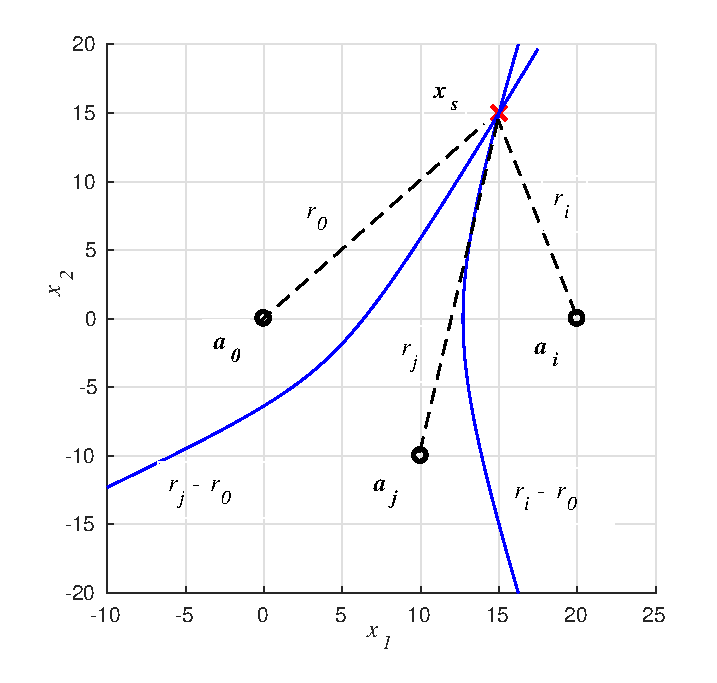
\includegraphics[height=0.45\textheight]{figures/socp_rd/TDOA_example}
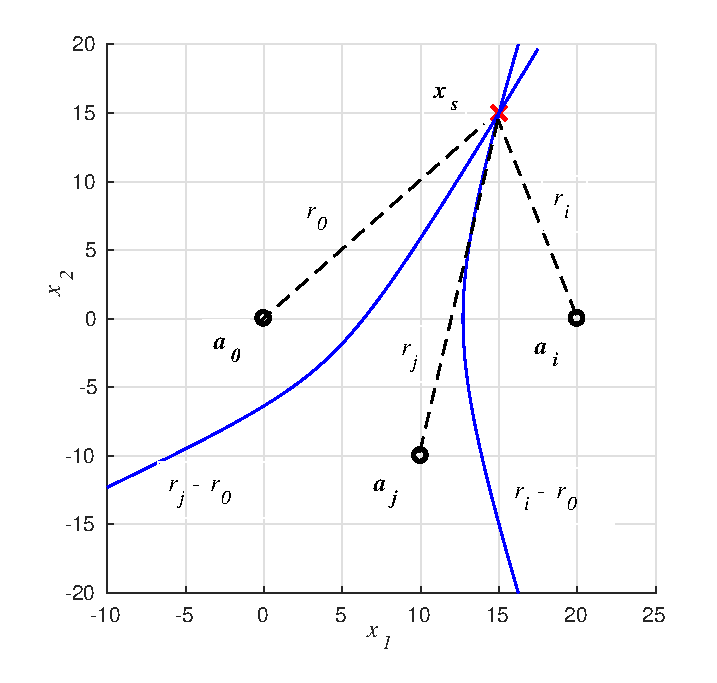
\includegraphics{figures/socp_rd/TDOA_example}
\caption{Range-difference localization.  At least three base stations are required for the planar localization. The red cross indicates the location of the signal source. Sensors are placed at $\protect\Ba_i = (20, 0)^T$, $\protect\Ba_j = (10, -10)^T$, and  $\protect\Ba_0$ is the reference sensor. The time (range) differences $r_j - r_0$ and $r_i - r_0$ form two hyperboloids with focii located at $\protect\Ba_i, \protect\Ba_j$ and $\protect\Ba_0$. Note that the hyperboloids are actually double sheeted, but for visual clarity only the halves which are part of the solution are shown. The intersection of these hyperboloids is the estimated position.
The figure depicts the locus of possible source locations as one half of a two-sheeted hyperboloids.}
\label{fig:tdoa}
\end{figure*}
%
% \phantom{m}
%An example of location estimation using TDOA is shown in Figure \ref{fig:hyperbola}. Consider an instance of the source localization problem on the plane $n = 2$ with the reference sensor $\Ba_0$ placed at the origin and five sensors $m = 5$ located at 
%\begin{equation}
%\nonumber
%\Ba_1 = \begin{bmatrix}
%-5 \\ -13
%\end{bmatrix}, \
%\Ba_2 = \begin{bmatrix}
%-12 \\ 1
%\end{bmatrix},  \
%\Ba_3 = \begin{bmatrix}
%-1 \\ -5
%\end{bmatrix}, \
%\Ba_4 = \begin{bmatrix}
%-9 \\ -12
%\end{bmatrix}, \
%\Ba_5 = \begin{bmatrix}
%-3 \\ -12
%\end{bmatrix}
%\\
%\end{equation}
%
%The source emitting the signal was located at $\Bx_s = (-5,11)^T$. Figure \ref{fig:hyperbola} depicts the locus of possible source locations as one half of a two-sheeted hyperboloids.

%\begin{figure} 
%\centering
%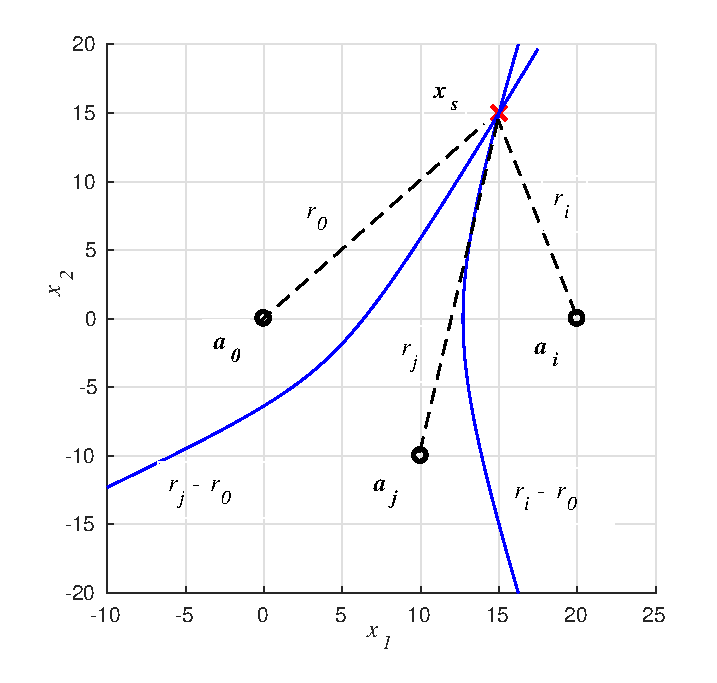
\includegraphics{figures/socp_rd/TDOA_example}
%\caption{Algorithm and contours of the R-LS objective function over the region $\protect\Re = \protect\lbrace \protect\Bx:-15\protect\leq x_1 \protect\leq 15, -25\protect\leq x_2 \protect\leq 15 \protect\rbrace$. The red cross indicates the location of the signal source. Sensors are located at $(-5, -13)^T$, $(-12, 1)^T$, $(-1, -5)^T$, $(-9, -12)^T$ and  $(-3, -12)^T$. Hyperbolas denote possible source locations given the pairwise range-difference readings. Large circles denote possible source locations given the noisy range reading at a particular sensor.}
%\label{fig:hyperbola}
%\end{figure}
 
%Given two base station locations $BS_i$ and $BS_0$, placed at $\Ba_i$ and $\Ba_0$ respectively, with $BS_0$ placed at the origin of the coordinate system, i.e. $\Ba_0 = \symb{0}_n$, and used as a reference station, and a known TDOA, the locus of possible source locations is one half of a two-sheeted hyperboloid. Consider now a third base station $BS_j$ at a third location. This would provide one extra independed TDOA measurement and the source is located on the curve determined by the two intersecting hyperboloids.

%Each TDOA measurement constrains the location of the signal source to be on a hyperboloid with a constant range-difference between the two reference points.

%\textit{Matlab} Using the arrival times, the time differences of arrival between each pair of eNodeBs is calculated using hPositioningTDOA.m. The particular time difference of arrival between a pair of eNodeBs can result from the UE being located at any position where two circles, each centered on an eNodeB, intersect. The two circles have radii which differ by the distance covered at the speed of light in the given time difference. The complete set of possible UE positions across all possible radii for one circle (with the other circle maintaining a radius appropriate to the time difference as already described) forms a hyperbola. The "hyperbolas of constant delay difference" for all the different pairs of eNodeBs are plotted relative to the known eNodeB positions and intersect at the position of the UE.
%A hyperbola is the basis for solving multilateration problems, the task of locating a point from the differences in its distances to given points — or, equivalently, the difference in arrival times of synchronized signals between the point and the given points. Such problems are important in navigation, particularly on water; a ship can locate its position from the difference in arrival times of signals from a LORAN or GPS transmitters. Conversely, a homing beacon or any transmitter can be located by comparing the arrival times of its signals at two separate receiving stations; such techniques may be used to track objects and people. In particular, the set of possible positions of a point that has a distance difference of 2a from two given points is a hyperbola of vertex separation 2a whose foci are the two given points.

%\textit{Wiki} If a pulse is emitted from a platform, it will generally arrive at slightly different times at two spatially separated receiver sites, the TDOA being due to the different distances of each receiver from the platform. In fact, for given locations of the two receivers, a whole set of emitter locations would give the same measurement of TDOA. Given two receiver locations and a known TDOA, the locus of possible emitter locations is one half of a two-sheeted hyperboloid.

%\textit{Wiki} In simple terms, with two receivers at known locations, an emitter can be located onto a hyperboloid.[1] Note that the receivers do not need to know the absolute time at which the pulse was transmitted – only the time difference is needed. A fourth receiver is needed for another independed TDOA, this wil give an extra hyperboloid, the intersection of the curve with this hyperboloid gives one or two solutions, the emitter is then located at the one or at the one of the two solutions.



The localization problem discussed in this section involves a given array of $m+1$ sensors placed in the $n = 2$ or 3 dimensional space with coordinates specified by $\{\Ba_1, \Ba_2, . . . , \Ba_m , a_i \in R^n\}$ and  $\Ba_0 = \symb{0}_n$ placed at the origin and used as a reference sensor. The localization problem here is to estimate the location of a radiating source $\Bx$ given the locations of the $m+1$ sensors and noise-contaminated range-difference measurements $\{d_i, i = 1, 2, \ldots, m\}$ where 
\setcounter{abc}{0}
\begin{equation} \label{eq:6.1}
d_i = \|\Bx - \Ba_i\| - \|\Bx\| + \varepsilon_i, \mbox{ for } i = 1, 2, \ldots, m
\end{equation}
Therefore, the standard range-difference LS (RD-LS) problem is formulated as
\begin{equation} \label{eq:6.2}
\Min \sum^m_{i=1}\left( \|\Bx - \Ba_i\| - \|\Bx\| - d_i\right)^2
\end{equation}
As described in Sec.2.2 of the thesis, finding the solution to ($\ref{eq:6.2}$) is a non-trivial problem and many approaches have been developed to address it. In the following we propose a new iterative procedure to tackle the RD-LS problem (\ref{eq:6.2}), with the goal of achieving a more accurate and robust solution. The central part of the procedure is a convex quadratic programming (QP) problem that needs to be solved in each iteration to provide an increment vector that updates the present iterate to next towards the solution of the localization problem at hand.

\subsection{Sequential Convex Relaxation}

%\newpage 
%
%\input chapters/5/scp_rd_ls
%
%\newpage

We begin by re-writing the unconstrained problem in (\ref{eq:6.2}) as a constrained problem with second-order cone constraints%can be equivalently written as
\setcounter{abc}{0}
\begin{eqnarray} \label{eq:6.3} %1.7
\stepcounter{abc}
\setcounter{equation}{3}
\Min_{\Bx, y, \Bz} & & \sum^m_{i=1}\left( z_i - y - d_i\right)^2\\
\stepcounter{abc}
\setcounter{equation}{3}
\mbox{subject to:}& &\|\Bx - \Ba_i\| = z_i, \quad  i = 1, 2, \ldots m \\
\stepcounter{abc}
\setcounter{equation}{3}
& &\|\Bx\|  = y
\end{eqnarray}
Assume we are in the $k$th iteration and we are to update the $k$th iterate $\{\Bx_k,y_k,\Bz_k\}$. Let the next iterate be
\setcounter{abc}{0}
\begin{eqnarray} \label{eq:6.4} %1.8
\stepcounter{abc}
\Bx^{k+1} &=& \Bx^k + \Bdelta_x \\
\stepcounter{abc}
\setcounter{equation}{4}
y^{k+1} &=& y^k + \delta_y \\
\stepcounter{abc}
\setcounter{equation}{4}
\Bz^{k+1} &=& \Bz^k + \Bdelta_z
\end{eqnarray}
where $\{\Bdelta_x, \delta_y, \Bdelta_z\}$
are such that the objective function in (
\ref{eq:6.4}a) is reduced and, at the same time, the constraints in (\ref{eq:6.3}b) and (\ref{eq:6.3}c) are better approximated at $\{\Bx_{k+1},y_{k+1},\Bz_{k+1}\}$ in the sense that
\setcounter{abc}{0}
\begin{eqnarray}
\nonumber
\|\Bx_{k+1} - \Ba_i\| &\approx &z_i^{k+1}, \quad i = 1, 2, \ldots, m \\
\nonumber
\|\Bx_{k+1}\| &\approx &y_{k+1}
\end{eqnarray}
namely,
\setcounter{abc}{0}
\begin{eqnarray}
\nonumber
\|\Bx_{k} + \Bdelta_x - \Ba_i\| &\approx &z_i^{k} + \Bdelta_{z_i}, \quad i = 1, 2, \ldots, m \\
\nonumber
\|\Bx_{k} + \Bdelta_x\| &\approx &y_{k}  + \Bdelta_y
\end{eqnarray}
By replacing the left-hand sides of the above equations with their first-order Taylor approximations, we obtain
\setcounter{abc}{0}
\begin{eqnarray}
\nonumber
\|\Bx_{k} - \Ba_i\| + \partial_x^T\|\Bx_{k} - \Ba_i\|\Bdelta_x &\approx & z_i^{k} + \Bdelta_{z_i}, \quad i = 1, 2, \ldots, m \\
\nonumber
\|\Bx_{k}\|  + \partial_x^T\|\Bx_{k}\|\Bdelta_x\ &\approx & y_{k}  + \Bdelta_y
\end{eqnarray}
where $\partial_x$ is the subdifferential operator with respect to variable $\Bx$. Assuming $\Bx_k \neq \Ba_i$ and $\Bx_k$ is nonzero, then
\begin{equation}
\nonumber
\partial_x\|\Bx_{k} - \Ba_i\| = \frac{\Bx_{k} - \Ba_i}{\|\Bx_{k} - \Ba_i\|} \ \mbox{and } \partial_x\|\Bx_{k}\| = \frac{\Bx_{k}}{\|\Bx_{k}\|}
\end{equation}
Hence
\setcounter{abc}{0}
\begin{eqnarray} \label{eq:6.5} %1.9
\stepcounter{abc}
\|\Bx_k - \Ba_i\| + \frac{\left(\Bx_{k} - \Ba_i\right)^T\Bdelta_x}{\|\Bx_k - \Ba_i\|} &\approx &z^{(k)}_i + \delta_{z_{j}}, \quad i = 1, 2,...,m \\
\stepcounter{abc}
\setcounter{equation}{5}
\|\Bx_k\| + \frac{\Bx_{k}^T\Bdelta_x}{\|\Bx_k\|} &\approx &y_k + \delta_y
\end{eqnarray}
The objective in (\ref{eq:6.3}a) can be written as
 \setcounter{abc}{0}
\begin{eqnarray} 
\nonumber
F(\Bx_{k+1}) & =  & \sum^m_{i = 1} \left(z^{(k)}_i + \delta_{z_i} - (y_k + \delta_y) - d_i \right)^2 \\
\nonumber
& = & \sum^m_{i = 1} \left(- \delta_y + \delta_{z_i}  - \tilde{d_i^{(k)}} \right)^2
\end{eqnarray}
where 
\begin{equation}
\nonumber
\tilde{d}^{(k)}_i =  d_i - y_k - z_i^{(k)}
\end{equation}
are grouped known constant terms. Based on the above, the problem to be solved in the \textit{k}th iteration is formulated as
\setcounter{abc}{0}
\begin{eqnarray} \label{eq:6.6} %1.10
\stepcounter{abc}
\Min_{\tilde{\Bdelta}}& &f(\tilde{\Bdelta}) = \sum^m_{i=1}\left(-\delta_y + \delta_{z_{j}} - \tilde{d^{(k)}_i}\right)^2\\
\stepcounter{abc}
\setcounter{equation}{6}
\mbox{subject to:}& &\|\Bx_k - \Ba_i\| + \frac{\left(\Bx_{k} - \Ba_i\right)^T\Bdelta_x}{\|\Bx_k - \Ba_i\| } = z_i^{(k)} + \delta_{z_{j}}, \\
\nonumber
& &\qquad \qquad \qquad \qquad \qquad \qquad \qquad  \qquad i = 1, 2, \ldots m \\
\stepcounter{abc}
\setcounter{equation}{6}
& &\|\Bx_k\| + \frac{\Bx_k^T\Bdelta_x}{\|\Bx_k\|} = y_k + \delta_y \\
\stepcounter{abc}
\setcounter{equation}{6}
& &\begin{bmatrix}
-\beta\BOne_2 \\
-\beta \\
-\beta\BOne_m
\end{bmatrix} \leq \begin{bmatrix}
\Bdelta_x \\
\delta_y \\
\Bdelta_z
\end{bmatrix} \leq \begin{bmatrix}
\beta\BOne_2 \\
\beta \\
\beta\BOne_m
\end{bmatrix}
\end{eqnarray}
The constraints in (\ref{eq:6.6}d) assure that the magnitude of each component in $\{\Bdelta_x, \delta_y, \Bdelta_z\}$ is no greater than $\beta$. %, but also they assure that all components of $\{y_{k + 1}, \Bz_{k + 1}\}$ are nonnegative as long as $\{y_{k}, \Bz_{k}\}$ are nonnegative, which are natural to impose as can be seen from (\ref{eq:6.3}b) and (\ref{eq:6.3}c) because they are vector norms. 
Obviously, the problem in (\ref{eq:6.6}) is a convex QP problem. One technical difficulty that may occur in solving problem (\ref{eq:6.6}) is that the feasible region defined by (\ref{eq:6.6}b), (\ref{eq:6.6}c), and (\ref{eq:6.6}d) may be empty. In such a case the constraints in problem (\ref{eq:6.6})
must be adequately relaxed in order for the problem to be solvable. To this end we express the problem in (\ref{eq:6.6}) in a more compact form as
\setcounter{abc}{0}
\begin{eqnarray} \label{eq:6.7} %1.11
\stepcounter{abc}
\Min_{\Bdelta}& &f\left(\tilde{\Bdelta}\right) \\
\stepcounter{abc}
\setcounter{equation}{7}
\mbox{subject to}& &\BA_k\tilde{\Bdelta} = \Bb_k \\
\stepcounter{abc}
\setcounter{equation}{7}
& &\BC\tilde{\Bdelta} \leq \Bq
\end{eqnarray}
where the objective function is
\setcounter{abc}{0}
\begin{eqnarray}
\nonumber
f\left(\tilde{\Bdelta}\right) = \|\BS\tilde{\Bdelta} - \tilde{\Bd_k} \|_2
 %\| -\delta_y\symb{1_m} + \Bdelta_z - \tilde{\Bd_k} \|_2
\end{eqnarray}
and
\setcounter{abc}{0}
\begin{equation}\label{eq:6.8}
\stepcounter{abc}
\BS = \begin{bmatrix}
\symb{0}_{m \times 1} & -\symb{1}_{m \times 1} & -\symb{I}_m
\end{bmatrix} , 
\tilde{\Bdelta} = \begin{bmatrix}
\Bdelta_x \\
\delta_y \\
\Bdelta_z
\end{bmatrix} , 
\BA_k = \begin{bmatrix}
\BA_1^{(k)} & \symb{0}_{m \times 1} & -\symb{I}_m \\
\Bx_k & -1 & \symb{0}_{1 \times m}\\
\end{bmatrix} 
\end{equation}
\setcounter{abc}{1}
\begin{equation}
\stepcounter{abc}
\setcounter{equation}{8}
\BA_1^{(k)} = \begin{bmatrix}
\frac{\left(\Bx_k - \Ba_1\right)^T}{\|\Bx_k - \Ba_1\|} \\
\frac{\left(\Bx_k - \Ba_2\right)^T}{\|\Bx_k - \Ba_2\|} \\
\vdots \\
\frac{\left(\Bx_k - \Ba_m\right)^T}{\|\Bx_k - \Ba_m\|} \\
\end{bmatrix}, 
\quad \Bb_k = \begin{bmatrix}
z_1^{(k)} - \|\Bx_k - \Ba_1\| \\
z_2^{(k)} - \|\Bx_k - \Ba_2\| \\
\vdots \\
z_m^{(k)} - \|\Bx_k - \Ba_m\| \\
y_k - \|\Bx_k\| \\
\end{bmatrix}
\end{equation}
\begin{equation}
\stepcounter{abc}
\setcounter{equation}{8}
\tilde{\Bd_k} = 
\begin{bmatrix}
d_1 + y^k - z_1^k \\
d_2 + y^k - z_2^k \\
\vdots \\
d_m + y^k - z_m^k \\
\end{bmatrix},
\BC = \begin{bmatrix}
\symb{I}_{m+3} \\
-\symb{I}_{m+3}
\end{bmatrix},
\Bq = \beta\Be
\end{equation}
\noindent
where $\Be = \symb{1}_{2(m+3)}$ is the all-one vector of dimension $2(m+3)$. By introducing nonnegative slack variables $\Bu, \Bv$, and $w$, we relax the problem in (\ref{eq:6.7}) to
\setcounter{abc}{0}
\begin{eqnarray} \label{eq:6.9} %1.12
\stepcounter{abc}
\Min_{\Bdelta}& &f\left(\tilde{\Bdelta}\right) + \tau\sum_{i=1}^{m+1} \left(u_i + v_i\right) +\tau w\\
\stepcounter{abc}
\setcounter{equation}{9}
\mbox{subject to}& &\BA_k\tilde{\Bdelta} - \Bb_k = \Bu - \Bv \\
\stepcounter{abc}
\setcounter{equation}{9}
& &\BC\tilde{\Bdelta} - \Bq \leq w\Be \\
\stepcounter{abc}
\setcounter{equation}{9}
& & \Bu \geq \symb{0}, \Bv \geq \symb{0}, w \geq 0
\end{eqnarray}
where $\tau > 0$ is a sufficiently large scalar. It is easy to verify that the feasible region defined by (\ref{eq:6.9}b) -  (\ref{eq:6.9}d) is always nonempty. For example, if we fix $\tilde{\Bdelta} = \tilde{\Bdelta_0}$ arbitrarily, then obviously the point $\{\tilde{\Bdelta_0}, \Bu_0, \Bv_0, w_0\}$ with
\setcounter{abc}{0}
\begin{equation}
\nonumber
\Bu_0 = \mbox{max}\{\symb{0},\BA_0\tilde{\Bdelta_0} -\Bb_0\}, \quad \Bv_0 = \mbox{max}\{\symb{0},-(\BA_0\tilde{\Bdelta_0} -\Bb_0)\}, \mbox{and } w_0 = \mbox{max}\{0,\BC\tilde{\Bdelta_0} -\Bq\}
\end{equation}

\noindent
is a feasible point for problem (\ref{eq:6.9}). Penalty terms $\tau\sum_{i=1}^{m+1} \left(u_i + v_i\right) +\tau w$ are included in the objective function in (\ref{eq:6.9}a) in order to reduce the magnitudes of the slack variables while minimizing the original objective function. If the solution slack variables turn out to be all zero, then the solution  of (\ref{eq:6.9}) also solves problem (\ref{eq:6.7}). Otherwise, we conclude that problem (\ref{eq:6.7}) in not solvable and the solution obtained by solving (\ref{eq:6.9}) is a reasonable candidate for the $k$th iteration to update $\{\Bx_k, y_k, \Bz_k\}$.

\subsection{The Algorithm}

The input parameters for the algorithm include the bound $\beta$ on the increment vector $\tilde{\Bdelta} =\left(
\Bdelta_x, \delta_y, \Bdelta_z\right)$. It controls the size of a "trust region" over which a convex subproblem is carried out and is responsible for the performance of the algorithm. If parameter $\beta$ is chosen too large, then approximation $\Bx_{k+1}$ will perform poorly because in this case the convex model is less accurate \cite{OPTII}. If $\beta$ is too small the progress of the algorithm will be too slow. In our simulations a $\beta$ between 3 and 6 was found to work very well. Other input parameters are initial point $\Bx_0$, initial weight for penalty terms $\tau_0$, and upper limit of the weight  $\tau_{max}$ (to avoid numerical problems that may occur  if $\tau_k$ becomes too large).

We remark that the method proposed in this section is \textit{local}, therefore is not guaranteed to converge to the global minimum when applied to the nonconvex problem. As discussed in Sec. 2.2 of the thesis, the original LS objective in (\ref{eq:6.2}) is highly nonconvex with many local minimums even for small-scale systems. Consequently, the choise of a good initial point is critical to ensure good performance of the method. Several techniques are available, these include: i) set the initial point to the origin; ii) select the initial point uniformly randomly over the same region as the unknown radiating source; iii) run the algorithm from a set of candidate initial points and identify the solution as the one with lowest LS error.  The candidate initial points can be selected either randomly over the region or based on some  a priori information, for example, the geometry of the sensor network; iv) solve an approximating problem or apply a “global” localization algorithm such as those in \cite{BeckStLi} to generate an approximate LS solution, then take it as the initial point to run the proposed algorithm. 

Based on the analysis above, the localization algorithm for range-difference measurements can be outlined as follows. For the ease of notation we will refer to the proposed algorithm as Sequential Convex Relaxation for Range-Difference-based Least Squares (SCR-RDLS).

%The constraint $\beta$ was imposed on each element of the vector $\tilde{\Bdelta}$ to guarantee that at each iteration is sufficiently small.

%Dropping the constraints in \ref{eq:6.8}f,g allows more variety in choosing the search direction, which increases the likelihood of the algorithm not to get trapped in the local minimimum.

\phantom{m}
\framebox{%
\parbox{5.4in}{
\label{alg:scp_rd}
\phantom{m}

\noindent \textbf{Algorithm 4. Sequential Convex Relaxation for Range-Difference Localization}

\phantom{m}

1) Input data: Sensor locations $\{\Ba_i, i=1,\ldots,m\}$, range-difference measurements $\{d_i, i=1,\ldots,m\}$, initial point $\Bx_0$, initial weight $\tau_0$ and upper limit of weight $\tau_{max}$, increment bound $\beta$ and convergence tolerance $\epsilon$. %\gamma, \sigma$, 
Set iteration count to $k = 0$. Form $\BS, \BC$ and $\Bq$ as
\setcounter{abc}{0}
\begin{equation}
\nonumber
\BS = \begin{bmatrix}
\symb{0}_{m \times 1} & -\symb{1}_{m \times 1} & -\symb{I}_m
\end{bmatrix},
\BC = \begin{bmatrix}
\symb{I}_{m+3} \\
-\symb{I}_{m+3}
\end{bmatrix},
\Bq = \beta\Be
\end{equation}
%\phantom{m}

2) Form $y_k$ and $\Bz_k$ as
\begin{equation}
\nonumber
y_k =\|\Bx_k\|, \Bz_k = \begin{bmatrix}
\|\Bx_k - \Ba_1\| \\
\vdots \\
\|\Bx_k - \Ba_m\|
\end{bmatrix} 
\end{equation}
form $\BA_k, \tilde{\Bd_k}, \Bb_k$ and $\BC_k $ as in (\ref{eq:6.8}) and solve
%\phantom{m}
%\noindent
\setcounter{abc}{0}
\begin{eqnarray} 
\nonumber
\Min_{\Bdelta}& &f\left(\tilde{\Bdelta}\right) + \tau_k\sum_{i=1}^{m+1} \left(u_i + v_i\right) +\tau_k w\\
\nonumber
\mbox{subject to}& &\BA_k\tilde{\Bdelta} - \Bb_k = \Bu - \Bv \\
\nonumber
& &\BC\tilde{\Bdelta} - \Bq \leq w\Be \\
\nonumber
& & \Bu \geq \symb{0}, \Bv \geq \symb{0}, w \geq 0
\end{eqnarray}
\noindent
Denote the solution as $\tilde{\Bdelta}_k = (\Bdelta_x^*, \delta_y^*, \Bdelta_z^*)$. 

%\phantom{m}

3) Update  $\tau_{k+1} $ = min $(1.5\tau_k, \tau_{max})$, set $k = k+1$. Update $\tilde{\Bx}^{*}$ to
\setcounter{abc}{0}
\begin{eqnarray} 
\nonumber
\Bx^{*} = \Bx^k + \Bdelta_x^* \\
\nonumber
y^{*} = y^k + \delta_y^* \\
\nonumber
\Bz^{*} = \Bz^k + \Bdelta_z^*
\end{eqnarray}

%\phantom{m}

4) If $\|\tilde{\Bdelta}_k\| \leq \epsilon$, terminate and output $\Bx^*$ as the solution; otherwise, set $\tilde{\Bx}_{k} = \Bx^{*}$  and repeat from Step 2. 

\phantom{m}
}
}

\subsection{Numerical Results}

Performance of the proposed algorithm was evaluated and compared with existing state-of-the-art methods by Monte Carlo simulations with a set-up similar to that of \cite{BeckStLi}. SRD-LS solutions were used as performance benchmarks for the Algorithm 4. The sensor network consisted of $11$ sensors with $\Ba_0 = \BO$ placed at the origin and other ten sensors  $\{\Ba_i, i = 1, 2,\ldots,10\}$ randomly placed in the planar region in $[-15;15]\times[-15;15]$. A radiating source $\Bx_s$ was located randomly in the region $\{\Bx=[x_1;x_2], -10\leq x_1,x_2\leq 10\}$. The coordinates of the source and sensors were generated for each dimension following a uniform distribution. Measurement noise $\{\varepsilon_i, i=1,\ldots,m\}$ was modelled as independent and identically distributed (i.i.d) random variables with zero mean and variance $\sigma^2$, with $\sigma$ being one of four possible levels $\{10^{-3}, 10^{-2}, 10^{-1}, 1\}$.  The range-difference measurements $\{d_i, i=1, 2,\ldots,10\}$ were calculated using (\ref{eq:6.1}). Accuracy of source location estimation was evaluated in terms of average of the squared position error in the form $\|\Bx^*-\Bx_s\|^2$, where $\Bx_s$ denotes the exact source location and $\Bx^*$ is its estimation obtained by SRD-LS and proposed methods, respectively.  
In our simulations parameter $\beta$ was set to 3, the initial penalty term $\tau_0$, and upper limit of the penalty term $\tau_{max}$ were set to 10 and 10 000 respectively. The proposed method was implemented by using  CVX  \cite{cvx} and implementation of SRD-LS followed \cite{BeckStLi}. In our simulations we set the initial point $\Bx_0$ to the solution of the following subproblem
\setcounter{abc}{0}
\begin{eqnarray} \label{eq:initpnt}
\nonumber
\Min_{\Bx, y, \Bz} & &\sum^m_{i=1}\left( z_i - y - d_i\right)^2\\
\nonumber
\mbox{subject to:}& &\|\Bx - \Ba_i\| \leq z_i, \quad  i = 1, 2, \ldots m \\
\nonumber
& &\|\Bx\|  \leq y
\end{eqnarray}
\noindent
The iterations proceeded until the magnitude of the increment vector $\|\tilde{\Bdelta}_k\|$ falls below a convergence tolerance $\epsilon$ which was set to $\epsilon = 10^{-6}$. 

Table \ref{tab:scr_rdls}  provides comparisons of the SCR-RDLS with SRD-LS, where each entry is averaged squared error over 1,000 Monte Carlo runs of the method. %The MLE was implemented using Matlab function \textit{lsqnonlin} \cite{matlab}, initialized with the same point as PCCP.
 It is observed that, comparing with SRD-LS, the estimates produced by the proposed algorithm are found to be closer to the true source locations in MSE sense. The last column of the table  represents relative improvement (R.I.) of the proposed method over SRD-LS solutions in percentage. Further analysis of the data that was used to generate Table \ref{tab:scr_rdls} illustrates the advantage of the SCR-RDLS solution over the SRD-LS. 
Each entry in Table \ref{tab:rdls} is a standard deviation of the squared  estimation errors  aggregated over the  same 1,000 Monte Carlo runs described above in Table \ref{tab:scr_rdls} where the MSEs of the position estimation are shown. The results summarized in Table \ref{tab:rdls} indicate that the SCR-RDLS algorithm provides considerable performance improvement relative to the SRD-LS algorithm.

\phantom{m}

\begin{table}[h]
\centering
\caption{MSE of position estimation for SRD-LS and SCR-RDLS methods}
\phantom{m}
\begin{tabular}{|c|c|c|c|} \hline
\centering
$\sigma$ & SRD - LS & SCR-RDLS & (R.I.,\%)  \\ \hline
%&&& \\
1e-03&	1.2655e-06  & 8.4626e-07 &  33 \\ &&&\\
1e-02&	1.4492e-04 &  6.8385e-05 &  52 \\ &&&\\
1e-01&	1.3329e-02 & 7.1676e-03 &   46 \\ &&&\\
1e+0&	1.6077e+00 &  9.5371e-01 &   40  \\ %&&&\\
\hline
\end{tabular}
\label{tab:scr_rdls}
%\end{table}
%\begin{table}[h]

\phantom{m}

\centering
\caption{Standard deviation of the squared position estimation error for SRD-LS and SCR-RDLS methods}
\phantom{m}
\begin{tabular}{|c|c|c|} \hline
$\sigma$ & SRD - LS & SCR-RDLS  \\ \hline
%&&& \\ 
1e-03&	3.3990e-06 &  3.2917e-06 \\ &&\\
1e-02&	5.9818e-04 &   1.3673e-04 \\ &&\\
1e-01&	3.6154e-02  & 2.4337e-02 \\ &&\\
1e+0&	4.2206e+00 &  3.4931e+00 \\ %&&&&\\
\hline
\end{tabular}
\label{tab:rdls}
\end{table}

\phantom{m}

%\newpage
\input chapters/5/range_based


\section{Execution Time Comparison}

In this section we compare the average running time of the proposed algorithms for range and range-difference measurements. The algorithms have been implemented in Matlab using CVX [16] (Processor 1.8 GHz Intel Core i3, Memory 4 GB 1600 MHz DDR3). Each of the algorithms has been implemented using the initialization set-up described in the Numerical Results section of the relevant chapter. The noise level was set to $\sigma = 0.2$.

We run each algorithm 1000 times and compute the average execution time in milliseconds (Tables 4.5 and 4.7). Then we compare the running time with respect to the IRWSR-LS (Table 4.6) and IRWSRD-LS (Table 4.8). The complexity of IRWSR-LS (IRWSRD-LS) is that of the SR-LS (SRD-LS) times the number of re-weighting iterations. This approach is the fastest of all those proposed since at each iteration the solution is found in a closed form.  For the PCCP and SCR-RLS methods  each iteration involves solving an SOCP problem, and a convex QP problem in the case of SCR-RDLS.

\begin{table}[h]
\label{tab:absR}
\centering
\caption{Performance Comparison of Range-Based Algorithms. Absolute CPU time usage}
\phantom{m}
\begin{tabular}{|c|c|} 
\hline
Method &  Absolute time, ms.\\ \hline
%SR-LS & 1.1789e+00 \\&\\
IRWSR-LS  & 6.0777e+00 \\&\\
PCCP & 5.3790e+03 \\&\\
SCR-RLS & 3.7005e+03  \\ %&&&\\
\hline
\end{tabular}
%\begin{tabular}{||c||c|c|c||} 
%\hhline{|t:====:t|} 
%$\sigma$ & IRWSR-LS  & PCCP & SCR-RLS  \\ \hline
%%&&& \\
%1e-03&	  &   &   \\ &&&\\
%1e-02&	  &   &   \\ &&&\\
%1e-01&	  &   &    \\ &&&\\
%1e+0&	  &   &     \\ %&&&\\
%\hhline{|b:====:b|} 
%\end{tabular}
\end{table}


\begin{table}[h]
\label{tab:relR}
\centering
\caption{Performance Comparison of Range-Based Algorithms. Relative CPU time usage}
\phantom{m}
\begin{tabular}{|c|c|} 
\hline
Method &  Relative time\\ \hline
%SR-LS & 1 \\&\\
IRWSR-LS  & 1 \\&\\
PCCP & 885 \\&\\
SCR-RLS &  609  \\ %&&&\\
\hline
\end{tabular}
\end{table}



\begin{table}[h]
\label{tab:absRD}
\centering
\caption{Performance Comparison of Range-Difference-Based Algorithms. Absolute CPU time usage}
\phantom{m}
\begin{tabular}{|c|c|} 
\hline
Method &  Absolute time, ms.\\ \hline
%SRD-LS & 1.7581e+00 \\&\\
IRWSRD-LS  & 7.4039e+00 \\&\\
SCR-RDLS &  3.6347e+03  \\ %&&&\\
\hline
\end{tabular}
\end{table}



\begin{table}[h]
\label{relRD}
\centering
\caption{Performance Comparison of Range-Difference-Based Algorithms. CPU time usage}
\phantom{m}
\begin{tabular}{|c|c|} 
\hline
Method &  Relative time\\ \hline
%SRD-LS & 1 \\&\\
 IRWSRD-LS  & 1 \\&\\
SCR-RDLS &  490  \\ %&&&\\
\hline
\end{tabular}
\end{table}

%	\startchapter{Conclusion}

\section{Conclusion}


\section{Future Work}

Influense of sensor geometry on the accuracy of the proposed methods. For example, one of the highest impacts on accuracy degradation is Geometric Dilusion of Presicion. Optimum sensor arrangement is a separate research area. 

Multi-source localization, when the range measurements were obtained from the energy-based readings. 
	\appendix
%	\startappendix{}
\label{chapter:app1}

\section{Solving \ref{eq:3.16}}

% TODO reword as this is too similar to contents of paper 'original.pdf'
Next we show how to compute an exact solution to the SR-LS problem
(\ref{eq:3.16}). Note that \ref{eq:3.16} belongs to the class of problems
consisting of minimizing a quadratic function subject to a single
quadratic constraint. Problems of this type are called generalized trust
region subproblems (GTRS) \cite{More}. GTRS problems, although usually 
nonconvex, possess necessary and sufficient optimality conditions from
which efficient solution methods can be derived. In particular, by 
Theorem 3.2 of \cite{More}, $\By \in R^{n+1}$ is an optimal solution
of \ref{eq:3.16} if and only if there exists $\lambda \in R^{n}$ 
such that

\begin{equation} \label{eq:A.1}
(\BA^{T}\BA + \lambda\BD)\By = \BA^{T}\Bb - \lambda\Bf
\end{equation}

\begin{equation} \label{eq:A.2}
\By^{T}\BD\By + 2\Bf^{T}\By = 0
\end{equation}

\begin{equation} \label{eq:A.3}
\BA^{T}\BA + \lambda\BD \geq 0
\end{equation}

It follows that the optimal solution of \ref{eq:3.16} is given by

\begin{equation} \label{eq:A.4}
\hat{\mathbf{y}}(\lambda) = (\BA^{T}\BA + \lambda\BD)^{-1}(\BA^{T}\Bb - \lambda\Bf)
\end{equation}

where $\lambda$ is the unique solution of

\begin{equation} 
\label{eq:A.5}
\varphi(\lambda) = 0, \lambda \in I
\end{equation}

and the function $\varphi$ is defined by

\begin{equation} \label{eq:A.6}
\varphi(\lambda) \equiv \hat{\mathbf{y}}(\lambda)^{T}\BD\hat{\mathbf{y}}(\lambda) + 2\Bf^{T}\hat{\mathbf{y}}(\lambda)
\end{equation}

The interval $I$ consists of all $\lambda$ for which 
$\BA^{T}\BA + \lambda\BD$ is positive definite, which immediately implies
that 

\begin{equation} \label{eq:A.7}
I = \left(-\dfrac{1}{\lambda_1(\BD,\BA^{T}\BA)}, \infty\right)
\end{equation}

Moreover, it is known by Theorem 5.2 of \cite{More} that
$\varphi(\lambda)$ is strictly decreasing over $I$ and therefore
a simple bisection algorithm can be used to find the optimal $\lambda$
over the interval $I$.

Note that we have limited the discussion to the case in which 
$\BA^{T}\BA + \lambda\BD$ is strictly positive definite, which is
equivalent to saying that the optimal $\lambda$ is different from
$-1/\lambda_1(\BD, \BA^{T}\BA)$. The case in which the optimal $\lambda$
is equal to $-1/\lambda_1(\BD, \BA^{T}\BA)$ is the so-called
``hard case'' of the GRTS problem \cite{FortinWol}, which can 
also be treated by a more refined analysis. However, the value 
$\lambda = -1/\lambda_1(\BD, \BA^{T}\BA)$ 
is very unlikely to occur both theoretically and practically
(it never occurred in the tens of thousands of simulations we 
have performed). Therefore, for the sake of simplicity, we have
tacitly assumed that $\BA^{T}\BA + \lambda\BD$
is positive semi-definite.

The procedure for calculating the SR-LS estimate is summarized next:

a) Use a bisection algorithm to obtain a solution $\lambda$ to (\ref{eq:A.5}).

b) The SR-LS estimate is given by the first $n$ components of the 
vector $\hat{\mathbf{y}}(\lambda)$ in \ref{eq:A.4}.

An alternative approach for computing the SR-LS estimate is considered
in \cite{CheungChan}. The method in \cite{CheungChan} consists of 
finding all the five roots
of the equation $\varphi(\lambda) = 0$ over the real line. This is done
by invoking a root finding procedure for polynomials of degree five.
In a second stage, the global optimal solution of SR-LS is chosen as
the best of the derived possible solutions. Interestingly, in the
above we proved that there is no need to find all the roots of
$\varphi(\lambda) = 0$ and that a simple bisection algorithm is 
sufficient.

\section{Simultaneous Matrix Diagonalization}

\begin{equation} \label{eq:A.5}
\Bv^{T}(\BB^{T}\BB)\Bv = \|\BB\Bv\|^{2} 
\end{equation}

$\BB^{T}\BB$ is at least PSD (full rank), ?? x ??

\begin{equation} \label{eq:A.6}
\BU^{T}\BB^{T}\BB\BU = \begin{bmatrix}
\lambda_1 & & 0 \\
 & \ddots & \\
0 & & \lambda_n
\end{bmatrix}
\end{equation}

$\BU^{T}\BC\BU$ is symmetric.

Non-symmetric square root (of $\BB^{T}\BB$):

\begin{equation} \label{eq:A.7}
\BU\begin{bmatrix}
\sqrt{\lambda_1} & & 0 \\
 & \ddots & \\
0 & & \sqrt{\lambda_n}
\end{bmatrix}
\end{equation}

Symmetric square root:

\begin{equation} \label{eq:A.8}
\BB^{T}\BB = \BU\begin{bmatrix}
\lambda_1 & & 0 \\
 & \ddots & \\
0 & & \lambda_n
\end{bmatrix}\BU^{T} = \BU\begin{bmatrix}
\sqrt{\lambda_1} & & 0 \\
 & \ddots & \\
0 & & \sqrt{\lambda_n}
\end{bmatrix}\BU^{T}\BU\begin{bmatrix}
\sqrt{\lambda_1} & & 0 \\
 & \ddots & \\
0 & & \sqrt{\lambda_n}
\end{bmatrix}\BU^{T}
\end{equation}

i.e.

\begin{equation} \label{eq:A.9}
\BB^{T}\BB = (\BB^{T}\BB)^{1/2}(\BB^{T}\BB)^{1/2}
\end{equation}

\begin{equation} \label{eq:A.10}
\BV(\BB^{T}\BB)^{-1/2}(\BB^{T}\BB)(\BB^{T}\BB)^{-1/2}\BV^{T} = \BV\BI\BV = \begin{bmatrix}
\gamma_1 & & 0 \\
 & \ddots & \\
0 & & \gamma_{n+1}
\end{bmatrix}
\end{equation}

Then for the matrix $\BC$:

\begin{equation} \label{eq:A.11}
\BV(\BB^{T}\BB)^{-1/2}\BC(\BB^{T}\BB)^{-1/2}\BV^{T} = \begin{bmatrix}
\delta_1 & & 0 \\
 & \ddots & \\
0 & & \delta_{n+1}
\end{bmatrix}
\end{equation}

where $\BV$ is orthogonal.

Hence the matrix $\BP$ we seek to compute is given by:

\begin{equation} \label{eq:A.12}
\BP = (\BB^T\BB)^{-1/2}\BV^T
\end{equation}

Share same eigenspace, i.e. the basis of the eigenspace is the same.

\begin{eqnarray}
\BP^{-1}\BA\BP = diag\{\lambda_A\} \\
\nonumber
\BP^{-1}\BB\BP = diag\{\lambda_B\}
\end{eqnarray}

Eigenspace $\BE_{\lambda A}$ of $\BA$ is equivalent to null 
space of $(\BA - \lambda_A\BI)$. 
Hence for $(\BB^T\BB)$ rank = 2 it is true
that

\begin{eqnarray}
\BA = \BV\BLambda_a\BV^T \\
\BB = \BV\BLambda_b\BV^T \\
\BB\BA = \BV\BLambda_b\BV^T\BV\BLambda_a\BV^T = \BV\BLambda_b\BLambda_a\BV^T \\
\Leftrightarrow \BA\BB = \BV\BLambda_a\BLambda_b\BV^T
\end{eqnarray}

for the case when $\BA\BB = \BB\BA$.

\begin{eqnarray}
\nonumber
\BA\BV = \BB\BV\BD \\
\nonumber
\BA = \BP\BLambda_a\BP^T \\
\nonumber
\BB = \BP\BLambda_b\BP^T \\
\nonumber
\BH\BP = \BP\BLambda_a \\
\nonumber
\BB\BP = \BP\BLambda_b \Rightarrow \BP = \BB^{-1}\BP\BLambda_b \\
\nonumber
\BA = \BB\BV\BD\BV^T \\
\nonumber
\BP\BLambda_a\BP^T = \BP\BLambda_b\BP^T\BV\BD\BV^T \\
\nonumber
\BA\BB^{-1}\BP\BLambda_b = \BB^{-1}\BP\BLambda_b\BLambda_a \\
\nonumber
\BB\BA\BB^{-1}\BP = \BP\BLambda_b\BLambda_a\BLambda_b^{-1} \\
\nonumber
\BA = \BP\BLambda_a\BP^T
\end{eqnarray}

Decomposition of $\BB^T\BB$:

\begin{eqnarray}
\nonumber
[\BV, \BD] = eig(\BB^T\BB) \\
\nonumber
\Bd = diag(\BD) \\
\nonumber
\Bd_1 = -1/\sqrt{\Bd} \\
\nonumber
\BD_1 = diag(\Bd_1) \\
\nonumber
\BS_{b+b} = \BV\BD_1\BV^T = (\BB^T\BB)^{-1/2} \\
\nonumber
[\BV, \Bh] = eig(\BS_{b+b}\BC\BS_{b+b}) \\
\nonumber
\BP = \BS_{b+b}\BV^T
\end{eqnarray}

To ensure that all computations were performed correctly,
the following should hold:

\begin{equation}
\BP^T\BB^T\BB\BP \equiv \BI
\end{equation}

\section{Solving \ref{eq:3.32}}

\subsection{Finding roots of the polynomial}

\begin{eqnarray}
\sum^{n+1}_{j=1} \frac{f^2_j\delta_j}{\left(\gamma_j+\lambda\delta_j\right)^2} = 0 \\
\nonumber
\Leftrightarrow \sum^{n+1}_{j=1} f^2_j\delta_j \prod^{n+1}_{k=1,k\neq j}\left(\gamma_k + \lambda_k\delta_k\right)^2 = 0 
\end{eqnarray}
For the planar case, i.e. n = 2
\begin{equation}
\nonumber
\begin{aligned}
& f^2_1\delta_1(1 + \lambda\delta_2)^2(1 + \lambda\delta_3)^2 + f^2_2\delta_2(1 + \lambda\delta_1)^2(1 + \lambda\delta_3)^2 + f^2_3\delta_3(1 + \lambda\delta_2)^2(1 + \lambda\delta_1)^2 \\ 
& = a_0 + \lambda a_1 + \lambda^2 a_2 + \lambda^3 a_3 + \lambda^4 a_4
\end{aligned}
\end{equation}

\begin{eqnarray}
\nonumber
a_0 = f^2_1\delta_1 + f^2_2\delta_2 + f^2_3\delta_3 \\
\nonumber
a_1 = f^2_1\delta_1(2\delta_2 + 2\delta_3) + f^2_2\delta_2(2\delta_1 + 2\delta_3) + f^2_3\delta_3(2\delta_1 + 2\delta_2) \\
\nonumber
a_2 = f^2_1\delta_1(\delta^2_2 + \delta^2_3 + 4\delta_2\delta_3) + f^2_2\delta^2_2(\delta^2_1 + \delta^2_3 + 4\delta_1\delta_3) + f^2_3\delta_3(\delta^2_1 + \delta^2_2 + 4\delta_1\delta_2) \\
\nonumber
a_3 = f^2_1\delta_12(\delta^2_3\delta_2 + \delta^2_2\delta_3) + f^2_2\delta_22(\delta_1\delta^2_3 + \delta^2_1\delta_3) + f^2_3\delta_32(\delta_1\delta^2_2 + \delta^2_1\delta_2) \\
\nonumber
a_4 = f^2_1\delta_1\delta^2_2\delta^2_3 + f^2_2\delta_2\delta^2_1\delta^2_3 + f^2_3\delta_3\delta^2_1\delta^2_2
\end{eqnarray}

3.32



% The style of bibliography exemplified here is the "plain",
% normally used in science theses. This is shown
% by the entry {plain} below. Substitute the
% appropriate bibliography style. See also the
% PDF file "InformationOnBibliographyStyles" in this
% directory for more choices.

% The Bibliography file is a BibTex file named
% UVicThesis.bib and called below

	\TOCadd{Bibliography}
	\bibliographystyle{plain}
%	\bibliography{UvicThesis}
	\begin{thebibliography}{99}


\bibitem{SmithAbel} \label{r1}
J. O. Smith and J. S. Abel, ``Closed-form least-squares source location estimation from range-difference measurements,'' {\em IEEE Trans. on Acoustic, Speech Signal Proc.}, vol. 12, pp. 1661--1669, Dec. 1987.

\bibitem{ShcauRob} \label{r4}
H. Schau and A. Robinson, ``Passive source localization employing intersecting spherical surfaces from time-of-arrival differences,'' {\em IEEE Trans. on Acoustic, Speech Signal Proc.}, vol. ASSP--35, pp. 1223--1225, Aug. 1987.

\bibitem{Yao} \label{r6}
K. Yao, R. Hudson, C. Reed, D. Chen, and F. Lorenzelli, ``Blind beamforming on a randomly distributed sensor array system,'' {\em IEEE J. Select. Areas Commun.}, vol. 16, pp. 1555-1567, Oct. 1998.

\bibitem{Sprito}
M. A. Sprito, ``On the accuracy of cellular mobile station location estimation,'' {\em IEEE Trans. on Veh. Technol.}, vol. 50, pp. 674-685, May 2001.

\bibitem{Huang} \label{3}
Y. Huang, J. Benesty, G. W. Elko, and R. M. Mersereau, ``Realtime passive source localization: A practical linear correction least-squares approach,'' {\em IEEE Trans. on Speech Audio Proc.}, vol. 9, no. 8, pp. 943-956, Nov. 2002.


\bibitem{CheungChan} \label{r9}
K. W. Cheung, H. C. So, W. K. Ma, and Y. T. Chan, ``Least squares algorithms for time-of-arrival-based mobile location,'' {\em IEEE Trans. on Signal Proc.}, vol. 52, no. 4, pp. 1121--1228, Apr. 2004.

\bibitem{LiHu} \label{r5}
D. Li and H. Hu, ``Energy-Based Collaborative Source Localization Using Acoustic Microsensor Array,'' in {\em EURASIP Journal on Applied Signal Proc.}, vol. 4, 321--337, 2003.
%D. Li and H. Hu, ``Least square solutions of energy based acoustic source localization problems,'' in {\em Proc. ICPPW}, 2004.

\bibitem{ShengHu}
X. Sheng and Y.-H. Hu, ``ML Multiple-source localization using acoustic energy measurements with wireless sensor networks,'' {\em IEEE Trans. on Signal Proc.}, vol. 53, no.1, pp. 44--53, Jan. 2005.

\bibitem{Saric}
Z. M. Saric, D. D. Kukolj, and N. D. Teslic, ``Acoustic source localization in wireless sensor network'', {\em Circuits Syst Signal Proc.}, vol. 29, pp. 837--856, 2010.

\bibitem{LuWuYan}
L. Lu, H.-C. Wu, K.Yan, and S.Iyengar, ``Robust expectation maximization algorithm for multiple wideband acoustic source localization  in  the  presence  of  nonuniform  noise  variances,'' {\em IEEE Sensors J.}, vol. 11, no. 3, pp. 536--544, Mar. 2011.

\bibitem{Cheung} \label{r7}
K.W. Cheung, W.K. Ma, and H.C. So, ``Accurate approximation algorithm for TOA-based maximum-likelihood mobile location using semidefinite programming,'' in {\em Proc. ICASSP}, vol. 2, pp. 145--148, 2004.

\bibitem{Sayed} \label{r10}
A. H. Sayed, A. Tarighat, and N. Khajehnouri, ``Network-based wireless location,'' {\em IEEE Signal Pro. Mag.}, vol. 22, no. 4, pp. 24--40, July 2005.

\bibitem{Chan} \label{r17}
Y. T. Chan, H. Y. C. Hang, and P. C. Ching, ``Exact and approximate maximum likelihood localization algorithms,'' {\em IEEE Trans. on Veh. Technol.}, vol. 55, no. 1, pp. 10--16, Jan. 2006.

\bibitem{StLi} \label{r14}
P. Stoica and J. Li, ``Source localization from range-difference measurements,'' {\em IEEE Signal Proc. Mag.}, vol. 23, pp. 63--65,69, Nov. 2006.

\bibitem{BeckStLi}
A. Beck, P. Stoica and J. Li,  ``Exact and approximate solutions of source localization problems,'' {\em IEEE Trans. on Signal Proc.}, vol. 56, no. 5, pp. 1770--1777, May 2008.

\bibitem{BeckTeCh}
A. Beck, M. Teboulle, and Z. Chikishev, ``Iterative minimization schemes for solving the single source localization problem,''  {\em SIAM J. Optim.}, vol. 19, no. 3, pp. 1397--1416, Nov. 2008.

\bibitem{Daub}
I. Daubechies, R. DeVore, M. Fornasier, and C. S. G\"unt\"urk, ``Iteratively reweighted least squares minimization for sparse recovery,'' {\em Comm. Pure Appl. Math.}, vol. 63, pp. 1--38, 2010.

\bibitem{BeckGPS}
A. Beck, and D. Pan, ``On the solution of the GPS localization and circle fitting problems,''  {\em SIAM J. Optim.}, vol. 22, no. 1, pp. 108--134, Jan. 2012.

\bibitem{Beck15}
A. Beck, ``On the convergence of alternating minimization for convex programming with applications to iteratively re-weighted least squares and decomposition schemes,''  {\em SIAM J. Optim.}, vol. 25, no. 1, pp. 185-209, Jan. 2015.

\bibitem{More} \label{r11}
J.J. More, ``Generalizations of the trust region subproblem,'' {\em Optim. Methods Softw.}, vol. 2, pp. 189--209, 1993.

\bibitem{FortinWol} \label{r15}
C. Fortin and H. Wolkowicz, ``The trust region subproblem and semidefinite programming,'' {\em Optim. Methods Softw.}, vol. 19, no.1, pp. 41--67, 2004.

\bibitem{RReg}
D.P. O'Leary, ``Robust regression computation using iteratively reweighted least squares,'' {\em SIAM J. Matrix Anal. Appl.}, vol. 11, no. 3, pp. 466--480, 1990.

\bibitem{GIRLS}
N. Bissantz, L. D\"umbgen, A. Munk, and B.  Stratmann, ``Convergence analysis of generalized iteratively reweighted least squares algorithms on convex function spaces,'' {\em SIAM J. Optim.}, vol. 19, no. 4, pp 1828--1845, 2009.


%\bibitem{Weiz}
%E. Weiszfeld, ``On the point for which the sum of the distances to n given points is minimum,'' {\em Ann. Oper. Res.,}, vol. 167, pp. 7--41, 2009; translated from the French original [Tohoku Math. J., 43 (1937), pp. 355--386] and annotated by F. Plastria.

\bibitem{classMDS} \label{r8}
K. W. Cheung and H. C. So, ``A multidimensional scaling framework for mobile location using time-of-arrival measurements,'' {\em IEEE Trans. on Signal Proc.}, vol. 53, no. 2, pp. 460--470, Feb. 2005.

\bibitem{fastMDS}
S. Qin, Q. Wan, and L.-F. Duan, ``Fast and efficient multidimentional scaling algorithm for mobile positioning,'' {\em IET Signal Processing}, vol. 6, no. 9, pp. 857--861, March 2012.

\bibitem{dwMDS}
J.A. Costa, N. Patwari, and A. O. Hero, ``Distributed weighted-multidimentional scaling for node localization in sensor networks,''ACD Trans. Sens. Netw., vol. 2, no. 1, pp. 39--64, 2006. 

\bibitem{genMDS}
H.C. So and F.K.W. Chan, ``Generalized Subspace Approach for Mobile Positioning With Time-of-Arrival Measurements,'' {\em IEEE Trans. on Signal Proc.}, vol. 55, no. 10, pp. 5103--5107, October 2007.

\bibitem{LiuSurvey}
H. Liu, H. Darabi, P. B, and J. Liu, ``Survey of Wireless Indoor Positioning Techniques and Systems,'' {\em IEEE Trans. on Systems, Man and Cybernetics. Part C: Applications and Revies}, vol. 37, no. 6, pp. 1067--1080, Nov. 2007.

\bibitem{LiuHuPan}
Y. Liu, Y.H. Hu, and Q. Pan, ``Distributed, Robust Acoustic Source Localization in a Wireless Sensor Network,'' {\em IEEE Trans. on Signal Proc.}, vol. 60, no. 8, pp. 4350--4359, Aug. 2012.

\bibitem{KimLeJe}
W. Kim, J. Lee, and G. Jee, ``The interior-point method for an optimal treatment of bias in trilateration location,'' {\em IEEE Trans. Veh. Technol.}, vol. 55, no. 4, pp. 1291--1301, Jul. 2006.

\bibitem{SMAC}
T. Qiao, S. Redfield, A. Abbasi, Z. Su, and H. Liu, ``Robust coarse position estimation for TDOA localization,'' {\em IEEE Wireless Commun. Lett.}, vol. 2, no. 6, pp. 623--626, Dec. 2013.

\bibitem{Yu}
A. L. Yuille and A. Rangarajan, ``The concave-convex procedure,' {\em Neural Computation}, vol. 15, no. 4, pp. 915--936, 2003.

\bibitem{LBoyd}
T. Lipp and S. Boyd, ``Variations and extensions of the convex-concave procedure,'' {\em Research Report}, Stanford University, Aug. 2014.

\bibitem{CCPConv}
G. R. Lanckreit and B. K. Sriperumbudur, ``On the convergence of the concave-convex procedure,'' in  {\em Advances in Neural Information Proc. Systems}, pp. 1759--1767, 2009.

\bibitem{CCPGlob}
Y. Kang, Z. Zhang, and W.-J. Li, ``On the global convergence of majorization minimization algorithms for nonconvex optimization problems,'' in {\em arXiv:
1504.07791v2}, 2015.

\bibitem{clock}
M. R. Gholami, S. Gezici, and E. G. Str\"om, ``TW-TOA based positioning in the presence of clock imperfections,'' {\em  Digital Signal Processing}, vol. 59, pp. 19--30, 2016.

\bibitem{UWB}
M. R. Gholami, E. G. Str\"om, F. Sottile, D. Dardari, A. Conti, S. Gezici, M. Rydstr\"om, and M. A. Spirito, ``Static positioning using UWB range measurements,'' in {\em Future Network and Mobile Summit Conference Proceedings}, %Florence,  
pp. 1--10, 2010.

\bibitem{DarWinUWB}
D. Dardari, A.Conti, U.J. Ferner, A. Giorgetti, and M.Z. Win, ``Ranging with ultrawide bandwidth signals in multipath environments,'' {\em Proceedings of the IEEE}, vol. 97, pp. 427--450, 2009.

\bibitem{RydstromUWB}
M. R. Gholami, E. G. Str\"om, and M. Rydstr\"om, ``Indoor sensor node positioning using UWB range measurements,'' in {\em 17th European Signal Processing Conference (Eusipco)}, pp. 1943--1947, 2009.

\bibitem{VBoyd} \label{r12}
L. Vandenberghe and S. Boyd, ``Semidefinite programming,'' {\em SIAM Rev.}, vol. 38, no. 1, pp. 40--95, Mar. 1996.

\bibitem{Har}
P. Hartman, ``On functions representable as a difference of convex functions,'' {\em Pacific Journal of Math}, vol. 9, no. 3, pp. 707--713, 1959.

\bibitem{AntonLu}
A. Antoniou and W.-S. Lu, {\em Practical Optimization: Algorithms and Engineering Applications}, Springer, New-York, 2007.

\bibitem{Nes}
Y. Nesterov, {\em Introductory Lectures on Convex Optimization}, Kluwer Academic Publishers, Boston, 2004.

\bibitem{GeoLoc}
C. Gentile, N. Alsindi, R. Raulefs, and C. Teolis, {\em Geolocation Techniques: Principles and Applications}, Springer, New-York, 2013.

\bibitem{LocAlg}
G. Mao and B. Fidan, {\em Localization Algorithms and Strategies for Wireless Sensor Networks: Monitoring and Surveillance Techniques for Target Tracking},  Hershey, PA: IGI Global, New-York, 2009.

\bibitem{OPTII}
W.-S. Lu, {\em ``Engineering Design by Optimization II''}, ELEC 573/603 Course Notes, University of Victoria, 2014.

\bibitem{cvx}
CVX Research, http://cvx.com/cvx, August 2012.

\bibitem{matlab}
The Mathworks Inc., http://mathworks.com, 2015.

\bibitem{IRWSg}
``Iterative re-weighting''

\bibitem{PCCP}
``Penalty Convex-Concave Procedure of Source Localization Problem,''

\bibitem{AGPS}

\bibitem{FB}
fitbit website

\bibitem{Garmin}
garmin website

\bibitem{Skyhook}
http://www.skyhookwireless.com/

\bibitem{CiscoWLA}
http://www.cisco.com/c/en/us/products/wireless/wireless-location-appliance/index.html

\bibitem{Guvenc2}
I. Guvenc, Y.T. Chan, H.Y.C. Hang, and P.C. Ching, ``Exact and approximate maximum likelihood localization algorithms'', {\em IEEE Trans. Veh. Technol.}, vol. 55, no. 1, pp. 10--16, 2006.

\bibitem{Guvenc}
I. Guvenc and C.-C Chong, ``A survey on TOA based wireless localization and NLOS mitigation techniques'', {\em IEEE Commun. Surv. Tutor.}, vol. 11, no. 3, 3rd Quarter, 2009.

\bibitem{HoML}
Y.T. Chan andK.C. Ho, ``A simple and efficient estimator for hyperbolic location'', {\em IEEE Trans. Signal
Process.}, vol. 42, no. 8, 1905--1915, 1994.

\end{thebibliography}

\end{document}
